\documentclass[twoside]{book}

% Packages required by doxygen
\usepackage{fixltx2e}
\usepackage{calc}
\usepackage{doxygen}
\usepackage[export]{adjustbox} % also loads graphicx
\usepackage{graphicx}
\usepackage[utf8]{inputenc}
\usepackage{makeidx}
\usepackage{multicol}
\usepackage{multirow}
\PassOptionsToPackage{warn}{textcomp}
\usepackage{textcomp}
\usepackage[nointegrals]{wasysym}
\usepackage[table]{xcolor}

% Font selection
\usepackage[T1]{fontenc}
\usepackage[scaled=.90]{helvet}
\usepackage{courier}
\usepackage{amssymb}
\usepackage{sectsty}
\renewcommand{\familydefault}{\sfdefault}
\allsectionsfont{%
  \fontseries{bc}\selectfont%
  \color{darkgray}%
}
\renewcommand{\DoxyLabelFont}{%
  \fontseries{bc}\selectfont%
  \color{darkgray}%
}
\newcommand{\+}{\discretionary{\mbox{\scriptsize$\hookleftarrow$}}{}{}}

% Page & text layout
\usepackage{geometry}
\geometry{%
  a4paper,%
  top=2.5cm,%
  bottom=2.5cm,%
  left=2.5cm,%
  right=2.5cm%
}
\tolerance=750
\hfuzz=15pt
\hbadness=750
\setlength{\emergencystretch}{15pt}
\setlength{\parindent}{0cm}
\setlength{\parskip}{3ex plus 2ex minus 2ex}
\makeatletter
\renewcommand{\paragraph}{%
  \@startsection{paragraph}{4}{0ex}{-1.0ex}{1.0ex}{%
    \normalfont\normalsize\bfseries\SS@parafont%
  }%
}
\renewcommand{\subparagraph}{%
  \@startsection{subparagraph}{5}{0ex}{-1.0ex}{1.0ex}{%
    \normalfont\normalsize\bfseries\SS@subparafont%
  }%
}
\makeatother

% Headers & footers
\usepackage{fancyhdr}
\pagestyle{fancyplain}
\fancyhead[LE]{\fancyplain{}{\bfseries\thepage}}
\fancyhead[CE]{\fancyplain{}{}}
\fancyhead[RE]{\fancyplain{}{\bfseries\leftmark}}
\fancyhead[LO]{\fancyplain{}{\bfseries\rightmark}}
\fancyhead[CO]{\fancyplain{}{}}
\fancyhead[RO]{\fancyplain{}{\bfseries\thepage}}
\fancyfoot[LE]{\fancyplain{}{}}
\fancyfoot[CE]{\fancyplain{}{}}
\fancyfoot[RE]{\fancyplain{}{\bfseries\scriptsize Generated by Doxygen }}
\fancyfoot[LO]{\fancyplain{}{\bfseries\scriptsize Generated by Doxygen }}
\fancyfoot[CO]{\fancyplain{}{}}
\fancyfoot[RO]{\fancyplain{}{}}
\renewcommand{\footrulewidth}{0.4pt}
\renewcommand{\chaptermark}[1]{%
  \markboth{#1}{}%
}
\renewcommand{\sectionmark}[1]{%
  \markright{\thesection\ #1}%
}

% Indices & bibliography
\usepackage{natbib}
\usepackage[titles]{tocloft}
\setcounter{tocdepth}{3}
\setcounter{secnumdepth}{5}
\makeindex

% Hyperlinks (required, but should be loaded last)
\usepackage{ifpdf}
\ifpdf
  \usepackage[pdftex,pagebackref=true]{hyperref}
\else
  \usepackage[ps2pdf,pagebackref=true]{hyperref}
\fi
\hypersetup{%
  colorlinks=true,%
  linkcolor=blue,%
  citecolor=blue,%
  unicode%
}

% Custom commands
\newcommand{\clearemptydoublepage}{%
  \newpage{\pagestyle{empty}\cleardoublepage}%
}

\usepackage{caption}
\captionsetup{labelsep=space,justification=centering,font={bf},singlelinecheck=off,skip=4pt,position=top}

%===== C O N T E N T S =====

\begin{document}

% Titlepage & ToC
\hypersetup{pageanchor=false,
             bookmarksnumbered=true,
             pdfencoding=unicode
            }
\pagenumbering{alph}
\begin{titlepage}
\vspace*{7cm}
\begin{center}%
{\Large My Project }\\
\vspace*{1cm}
{\large Generated by Doxygen 1.8.14}\\
\end{center}
\end{titlepage}
\clearemptydoublepage
\pagenumbering{roman}
\tableofcontents
\clearemptydoublepage
\pagenumbering{arabic}
\hypersetup{pageanchor=true}

%--- Begin generated contents ---
\chapter{Todo List}
\label{todo}
\Hypertarget{todo}

\begin{DoxyRefList}
\item[\label{todo__todo000003}%
\Hypertarget{todo__todo000003}%
Member \mbox{\hyperlink{class_c_g_1_1_base_connector_abd3e4f816a311c41418d5e090de2de15}{CG\+:\+:Base\+Connector\+:\+:stop}} ()]clean memory  
\item[\label{todo__todo000002}%
\Hypertarget{todo__todo000002}%
Class \mbox{\hyperlink{class_c_g_1_1_connect_config}{CG\+:\+:Connect\+Config}} ]none 
\end{DoxyRefList}
\chapter{Hierarchical Index}
\section{Class Hierarchy}
This inheritance list is sorted roughly, but not completely, alphabetically\+:\begin{DoxyCompactList}
\item \contentsline{section}{CG\+:\+:Base\+Connector}{\pageref{class_c_g_1_1_base_connector}}{}
\begin{DoxyCompactList}
\item \contentsline{section}{CG\+:\+:Base\+Client}{\pageref{class_c_g_1_1_base_client}}{}
\begin{DoxyCompactList}
\item \contentsline{section}{CG\+:\+:C\+G\+Client}{\pageref{class_c_g_1_1_c_g_client}}{}
\item \contentsline{section}{CG\+:\+:Client}{\pageref{class_c_g_1_1_client}}{}
\item \contentsline{section}{CG\+:\+:Peer}{\pageref{class_c_g_1_1_peer}}{}
\end{DoxyCompactList}
\item \contentsline{section}{CG\+:\+:Base\+Server}{\pageref{class_c_g_1_1_base_server}}{}
\begin{DoxyCompactList}
\item \contentsline{section}{CG\+:\+:C\+G\+Server}{\pageref{class_c_g_1_1_c_g_server}}{}
\item \contentsline{section}{CG\+:\+:Server}{\pageref{class_c_g_1_1_server}}{}
\end{DoxyCompactList}
\end{DoxyCompactList}
\item \contentsline{section}{Util\+:\+:Base\+Serialize}{\pageref{class_util_1_1_base_serialize}}{}
\begin{DoxyCompactList}
\item \contentsline{section}{Util\+:\+:Serialize}{\pageref{class_util_1_1_serialize}}{}
\begin{DoxyCompactList}
\item \contentsline{section}{CG\+:\+:Header}{\pageref{class_c_g_1_1_header}}{}
\item \contentsline{section}{CG\+:\+:Network\+Packet}{\pageref{class_c_g_1_1_network_packet}}{}
\begin{DoxyCompactList}
\item \contentsline{section}{CG\+:\+:Message\+Packet}{\pageref{class_c_g_1_1_message_packet}}{}
\end{DoxyCompactList}
\item \contentsline{section}{Util\+:\+:Int\+Packet}{\pageref{class_util_1_1_int_packet}}{}
\item \contentsline{section}{Util\+:\+:Test\+Packet}{\pageref{class_util_1_1_test_packet}}{}
\end{DoxyCompactList}
\item \contentsline{section}{Util\+:\+:Serialize\+Int16}{\pageref{class_util_1_1_serialize_int16}}{}
\item \contentsline{section}{Util\+:\+:Serialize\+Int32}{\pageref{class_util_1_1_serialize_int32}}{}
\item \contentsline{section}{Util\+:\+:Serialize\+Int32\+List}{\pageref{class_util_1_1_serialize_int32_list}}{}
\item \contentsline{section}{Util\+:\+:Serialize\+Int64}{\pageref{class_util_1_1_serialize_int64}}{}
\item \contentsline{section}{Util\+:\+:Serialize\+String}{\pageref{class_util_1_1_serialize_string}}{}
\end{DoxyCompactList}
\item \contentsline{section}{CG\+:\+:Buffer}{\pageref{class_c_g_1_1_buffer}}{}
\item \contentsline{section}{CG\+:\+:C\+G\+File\+Parser}{\pageref{class_c_g_1_1_c_g_file_parser}}{}
\item \contentsline{section}{CG\+:\+:C\+G\+Network\+Handler}{\pageref{class_c_g_1_1_c_g_network_handler}}{}
\item \contentsline{section}{CG\+:\+:Connect\+Config}{\pageref{class_c_g_1_1_connect_config}}{}
\begin{DoxyCompactList}
\item \contentsline{section}{CG\+:\+:Client\+Config}{\pageref{class_c_g_1_1_client_config}}{}
\item \contentsline{section}{CG\+:\+:Server\+Config}{\pageref{class_c_g_1_1_server_config}}{}
\end{DoxyCompactList}
\item \contentsline{section}{CG\+:\+:Connector\+Info}{\pageref{class_c_g_1_1_connector_info}}{}
\item \contentsline{section}{CG\+:\+:Data\+Packet}{\pageref{class_c_g_1_1_data_packet}}{}
\item \contentsline{section}{Util\+:\+:List$<$ T $>$}{\pageref{class_util_1_1_list}}{}
\begin{DoxyCompactList}
\item \contentsline{section}{Util\+:\+:M\+T\+List$<$ T $>$}{\pageref{class_util_1_1_m_t_list}}{}
\item \contentsline{section}{Util\+:\+:S\+T\+List$<$ T $>$}{\pageref{class_util_1_1_s_t_list}}{}
\end{DoxyCompactList}
\item \contentsline{section}{Util\+:\+:List$<$ CG\+:\+:Base\+Client $\ast$$>$}{\pageref{class_util_1_1_list}}{}
\item \contentsline{section}{Util\+:\+:List$<$ CG\+:\+:Base\+Server $\ast$$>$}{\pageref{class_util_1_1_list}}{}
\item \contentsline{section}{Util\+:\+:List$<$ std\+:\+:thread $\ast$$>$}{\pageref{class_util_1_1_list}}{}
\item \contentsline{section}{Util\+:\+:Lock}{\pageref{class_util_1_1_lock}}{}
\begin{DoxyCompactList}
\item \contentsline{section}{Log}{\pageref{class_log}}{}
\item \contentsline{section}{Util\+:\+:M\+T\+List$<$ T $>$}{\pageref{class_util_1_1_m_t_list}}{}
\end{DoxyCompactList}
\item \contentsline{section}{CG\+:\+:Network\+Handler}{\pageref{class_c_g_1_1_network_handler}}{}
\item \contentsline{section}{CG\+:\+:N\+P\+Serializer}{\pageref{class_c_g_1_1_n_p_serializer}}{}
\item \contentsline{section}{Util\+:\+:Object\+Pool$<$ T $>$}{\pageref{class_util_1_1_object_pool}}{}
\item \contentsline{section}{Util\+:\+:Object\+Pool$<$ CG\+:\+:Buffer $>$}{\pageref{class_util_1_1_object_pool}}{}
\item \contentsline{section}{Util\+:\+:Object\+Pool$<$ CG\+:\+:Connector\+Info $>$}{\pageref{class_util_1_1_object_pool}}{}
\item \contentsline{section}{Util\+:\+:Object\+Pool$<$ CG\+:\+:Data\+Packet $>$}{\pageref{class_util_1_1_object_pool}}{}
\item \contentsline{section}{CG\+:\+:Packet\+Function}{\pageref{class_c_g_1_1_packet_function}}{}
\item \contentsline{section}{Util\+:\+:Property$<$ T $>$}{\pageref{class_util_1_1_property}}{}
\item \contentsline{section}{Util\+:\+:Queue$<$ T $>$}{\pageref{class_util_1_1_queue}}{}
\begin{DoxyCompactList}
\item \contentsline{section}{Util\+:\+:B\+Queue$<$ T $>$}{\pageref{class_util_1_1_b_queue}}{}
\item \contentsline{section}{Util\+:\+:N\+B\+Queue$<$ T $>$}{\pageref{class_util_1_1_n_b_queue}}{}
\item \contentsline{section}{Util\+:\+:S\+T\+Queue$<$ T $>$}{\pageref{class_util_1_1_s_t_queue}}{}
\end{DoxyCompactList}
\item \contentsline{section}{Util\+:\+:Queue$<$ CG\+:\+:Buffer $\ast$$>$}{\pageref{class_util_1_1_queue}}{}
\item \contentsline{section}{Util\+:\+:Queue$<$ CG\+:\+:Connector\+Info $\ast$$>$}{\pageref{class_util_1_1_queue}}{}
\item \contentsline{section}{Util\+:\+:Queue$<$ CG\+:\+:Data\+Packet $\ast$$>$}{\pageref{class_util_1_1_queue}}{}
\item \contentsline{section}{Util\+:\+:Queue$<$ CG\+:\+:Timer $\ast$$>$}{\pageref{class_util_1_1_queue}}{}
\item \contentsline{section}{Util\+:\+:Queue$<$ T $\ast$$>$}{\pageref{class_util_1_1_queue}}{}
\item \contentsline{section}{Util\+:\+:Singleton$<$ T $>$}{\pageref{class_util_1_1_singleton}}{}
\item \contentsline{section}{Util\+:\+:Singleton$<$ Log $>$}{\pageref{class_util_1_1_singleton}}{}
\begin{DoxyCompactList}
\item \contentsline{section}{Log}{\pageref{class_log}}{}
\end{DoxyCompactList}
\item \contentsline{section}{Util\+:\+:Singleton$<$ Network $>$}{\pageref{class_util_1_1_singleton}}{}
\begin{DoxyCompactList}
\item \contentsline{section}{CG\+:\+:Network}{\pageref{class_c_g_1_1_network}}{}
\end{DoxyCompactList}
\item \contentsline{section}{Util\+:\+:Spin\+Lock}{\pageref{class_util_1_1_spin_lock}}{}
\begin{DoxyCompactList}
\item \contentsline{section}{Util\+:\+:N\+B\+Queue$<$ T $>$}{\pageref{class_util_1_1_n_b_queue}}{}
\end{DoxyCompactList}
\item \contentsline{section}{Util\+:\+:Thread}{\pageref{class_util_1_1_thread}}{}
\begin{DoxyCompactList}
\item \contentsline{section}{CG\+:\+:Worker\+Thread}{\pageref{class_c_g_1_1_worker_thread}}{}
\end{DoxyCompactList}
\item \contentsline{section}{CG\+:\+:Timer}{\pageref{class_c_g_1_1_timer}}{}
\end{DoxyCompactList}

\chapter{Class Index}
\section{Class List}
Here are the classes, structs, unions and interfaces with brief descriptions\+:\begin{DoxyCompactList}
\item\contentsline{section}{\mbox{\hyperlink{class_c_g_1_1_base_client}{C\+G\+::\+Base\+Client}} \\*This is a base class to make child client class that can use developers }{\pageref{class_c_g_1_1_base_client}}{}
\item\contentsline{section}{\mbox{\hyperlink{class_c_g_1_1_base_connector}{C\+G\+::\+Base\+Connector}} \\*This is a base class to make child class that can use developers }{\pageref{class_c_g_1_1_base_connector}}{}
\item\contentsline{section}{\mbox{\hyperlink{class_util_1_1_base_serialize}{Util\+::\+Base\+Serialize}} \\*Test }{\pageref{class_util_1_1_base_serialize}}{}
\item\contentsline{section}{\mbox{\hyperlink{class_c_g_1_1_base_server}{C\+G\+::\+Base\+Server}} \\*This is a base class to make child server class that can use developers }{\pageref{class_c_g_1_1_base_server}}{}
\item\contentsline{section}{\mbox{\hyperlink{class_util_1_1_b_queue}{Util\+::\+B\+Queue$<$ T $>$}} }{\pageref{class_util_1_1_b_queue}}{}
\item\contentsline{section}{\mbox{\hyperlink{class_c_g_1_1_buffer}{C\+G\+::\+Buffer}} \\*\mbox{\hyperlink{class_c_g_1_1_buffer}{Buffer}} that move receive data, storage non-\/finished data }{\pageref{class_c_g_1_1_buffer}}{}
\item\contentsline{section}{\mbox{\hyperlink{class_c_g_1_1_c_g_client}{C\+G\+::\+C\+G\+Client}} }{\pageref{class_c_g_1_1_c_g_client}}{}
\item\contentsline{section}{\mbox{\hyperlink{class_c_g_1_1_c_g_file_parser}{C\+G\+::\+C\+G\+File\+Parser}} \\*Convert file to use in cpp source }{\pageref{class_c_g_1_1_c_g_file_parser}}{}
\item\contentsline{section}{\mbox{\hyperlink{class_c_g_1_1_c_g_network_handler}{C\+G\+::\+C\+G\+Network\+Handler}} }{\pageref{class_c_g_1_1_c_g_network_handler}}{}
\item\contentsline{section}{\mbox{\hyperlink{class_c_g_1_1_c_g_server}{C\+G\+::\+C\+G\+Server}} }{\pageref{class_c_g_1_1_c_g_server}}{}
\item\contentsline{section}{\mbox{\hyperlink{class_c_g_1_1_client}{C\+G\+::\+Client}} }{\pageref{class_c_g_1_1_client}}{}
\item\contentsline{section}{\mbox{\hyperlink{class_c_g_1_1_client_config}{C\+G\+::\+Client\+Config}} \\*It is client config. same with connect\+Config but it will storage additional client infomation later }{\pageref{class_c_g_1_1_client_config}}{}
\item\contentsline{section}{\mbox{\hyperlink{class_c_g_1_1_connect_config}{C\+G\+::\+Connect\+Config}} \\*Set ip, port to connect with other }{\pageref{class_c_g_1_1_connect_config}}{}
\item\contentsline{section}{\mbox{\hyperlink{class_c_g_1_1_connector_info}{C\+G\+::\+Connector\+Info}} \\*If someone connect with me, create this. this class include connector info }{\pageref{class_c_g_1_1_connector_info}}{}
\item\contentsline{section}{\mbox{\hyperlink{class_c_g_1_1_data_packet}{C\+G\+::\+Data\+Packet}} }{\pageref{class_c_g_1_1_data_packet}}{}
\item\contentsline{section}{\mbox{\hyperlink{class_c_g_1_1_header}{C\+G\+::\+Header}} }{\pageref{class_c_g_1_1_header}}{}
\item\contentsline{section}{\mbox{\hyperlink{class_util_1_1_int_packet}{Util\+::\+Int\+Packet}} }{\pageref{class_util_1_1_int_packet}}{}
\item\contentsline{section}{\mbox{\hyperlink{class_util_1_1_list}{Util\+::\+List$<$ T $>$}} }{\pageref{class_util_1_1_list}}{}
\item\contentsline{section}{\mbox{\hyperlink{class_util_1_1_lock}{Util\+::\+Lock}} }{\pageref{class_util_1_1_lock}}{}
\item\contentsline{section}{\mbox{\hyperlink{class_log}{Log}} }{\pageref{class_log}}{}
\item\contentsline{section}{\mbox{\hyperlink{class_c_g_1_1_message_packet}{C\+G\+::\+Message\+Packet}} }{\pageref{class_c_g_1_1_message_packet}}{}
\item\contentsline{section}{\mbox{\hyperlink{class_util_1_1_m_t_list}{Util\+::\+M\+T\+List$<$ T $>$}} }{\pageref{class_util_1_1_m_t_list}}{}
\item\contentsline{section}{\mbox{\hyperlink{class_util_1_1_n_b_queue}{Util\+::\+N\+B\+Queue$<$ T $>$}} }{\pageref{class_util_1_1_n_b_queue}}{}
\item\contentsline{section}{\mbox{\hyperlink{class_c_g_1_1_network}{C\+G\+::\+Network}} }{\pageref{class_c_g_1_1_network}}{}
\item\contentsline{section}{\mbox{\hyperlink{class_c_g_1_1_network_handler}{C\+G\+::\+Network\+Handler}} }{\pageref{class_c_g_1_1_network_handler}}{}
\item\contentsline{section}{\mbox{\hyperlink{class_c_g_1_1_network_packet}{C\+G\+::\+Network\+Packet}} }{\pageref{class_c_g_1_1_network_packet}}{}
\item\contentsline{section}{\mbox{\hyperlink{class_c_g_1_1_n_p_serializer}{C\+G\+::\+N\+P\+Serializer}} }{\pageref{class_c_g_1_1_n_p_serializer}}{}
\item\contentsline{section}{\mbox{\hyperlink{class_util_1_1_object_pool}{Util\+::\+Object\+Pool$<$ T $>$}} }{\pageref{class_util_1_1_object_pool}}{}
\item\contentsline{section}{\mbox{\hyperlink{class_c_g_1_1_packet_function}{C\+G\+::\+Packet\+Function}} }{\pageref{class_c_g_1_1_packet_function}}{}
\item\contentsline{section}{\mbox{\hyperlink{class_c_g_1_1_peer}{C\+G\+::\+Peer}} }{\pageref{class_c_g_1_1_peer}}{}
\item\contentsline{section}{\mbox{\hyperlink{class_util_1_1_property}{Util\+::\+Property$<$ T $>$}} }{\pageref{class_util_1_1_property}}{}
\item\contentsline{section}{\mbox{\hyperlink{class_util_1_1_queue}{Util\+::\+Queue$<$ T $>$}} }{\pageref{class_util_1_1_queue}}{}
\item\contentsline{section}{\mbox{\hyperlink{class_util_1_1_serialize}{Util\+::\+Serialize}} }{\pageref{class_util_1_1_serialize}}{}
\item\contentsline{section}{\mbox{\hyperlink{class_util_1_1_serialize_int16}{Util\+::\+Serialize\+Int16}} }{\pageref{class_util_1_1_serialize_int16}}{}
\item\contentsline{section}{\mbox{\hyperlink{class_util_1_1_serialize_int32}{Util\+::\+Serialize\+Int32}} }{\pageref{class_util_1_1_serialize_int32}}{}
\item\contentsline{section}{\mbox{\hyperlink{class_util_1_1_serialize_int32_list}{Util\+::\+Serialize\+Int32\+List}} }{\pageref{class_util_1_1_serialize_int32_list}}{}
\item\contentsline{section}{\mbox{\hyperlink{class_util_1_1_serialize_int64}{Util\+::\+Serialize\+Int64}} }{\pageref{class_util_1_1_serialize_int64}}{}
\item\contentsline{section}{\mbox{\hyperlink{class_util_1_1_serialize_string}{Util\+::\+Serialize\+String}} }{\pageref{class_util_1_1_serialize_string}}{}
\item\contentsline{section}{\mbox{\hyperlink{class_c_g_1_1_server}{C\+G\+::\+Server}} }{\pageref{class_c_g_1_1_server}}{}
\item\contentsline{section}{\mbox{\hyperlink{class_c_g_1_1_server_config}{C\+G\+::\+Server\+Config}} \\*It is client config. same with connect\+Config but it will storage additional server infomation later }{\pageref{class_c_g_1_1_server_config}}{}
\item\contentsline{section}{\mbox{\hyperlink{class_util_1_1_singleton}{Util\+::\+Singleton$<$ T $>$}} }{\pageref{class_util_1_1_singleton}}{}
\item\contentsline{section}{\mbox{\hyperlink{class_util_1_1_spin_lock}{Util\+::\+Spin\+Lock}} }{\pageref{class_util_1_1_spin_lock}}{}
\item\contentsline{section}{\mbox{\hyperlink{class_util_1_1_s_t_list}{Util\+::\+S\+T\+List$<$ T $>$}} }{\pageref{class_util_1_1_s_t_list}}{}
\item\contentsline{section}{\mbox{\hyperlink{class_util_1_1_s_t_queue}{Util\+::\+S\+T\+Queue$<$ T $>$}} }{\pageref{class_util_1_1_s_t_queue}}{}
\item\contentsline{section}{\mbox{\hyperlink{class_util_1_1_test_packet}{Util\+::\+Test\+Packet}} }{\pageref{class_util_1_1_test_packet}}{}
\item\contentsline{section}{\mbox{\hyperlink{class_util_1_1_thread}{Util\+::\+Thread}} }{\pageref{class_util_1_1_thread}}{}
\item\contentsline{section}{\mbox{\hyperlink{class_c_g_1_1_timer}{C\+G\+::\+Timer}} \\*If you want to regist timer, using this }{\pageref{class_c_g_1_1_timer}}{}
\item\contentsline{section}{\mbox{\hyperlink{class_c_g_1_1_worker_thread}{C\+G\+::\+Worker\+Thread}} }{\pageref{class_c_g_1_1_worker_thread}}{}
\end{DoxyCompactList}

\chapter{Class Documentation}
\hypertarget{class_c_g_1_1_base_client}{}\section{CG\+:\+:Base\+Client Class Reference}
\label{class_c_g_1_1_base_client}\index{C\+G\+::\+Base\+Client@{C\+G\+::\+Base\+Client}}


This is a base class to make child client class that can use developers.  




{\ttfamily \#include $<$Base\+Client.\+h$>$}

Inheritance diagram for CG\+:\+:Base\+Client\+:\begin{figure}[H]
\begin{center}
\leavevmode
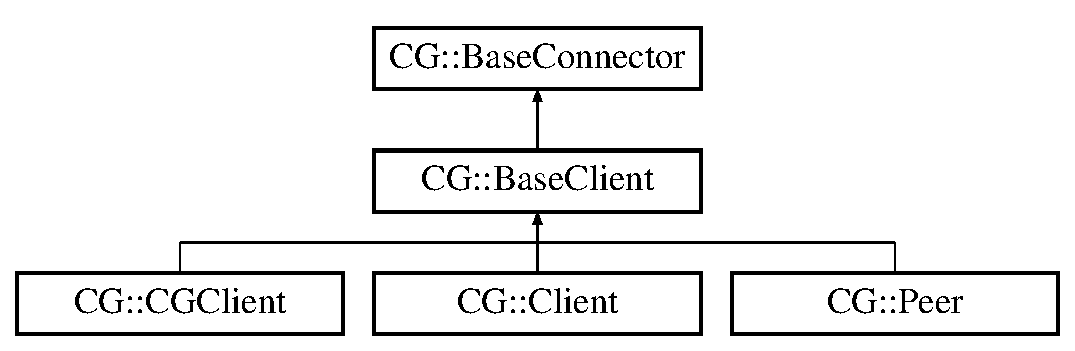
\includegraphics[height=3.000000cm]{class_c_g_1_1_base_client}
\end{center}
\end{figure}
\subsection*{Protected Member Functions}
\begin{DoxyCompactItemize}
\item 
\mbox{\Hypertarget{class_c_g_1_1_base_client_ade64ddce7c3af76c9a4be5fa685bca4d}\label{class_c_g_1_1_base_client_ade64ddce7c3af76c9a4be5fa685bca4d}} 
\mbox{\hyperlink{class_c_g_1_1_base_client_ade64ddce7c3af76c9a4be5fa685bca4d}{Base\+Client}} ()
\begin{DoxyCompactList}\small\item\em set client-\/type \end{DoxyCompactList}\end{DoxyCompactItemize}
\subsection*{Additional Inherited Members}


\subsection{Detailed Description}
This is a base class to make child client class that can use developers. 

\begin{DoxyAuthor}{Author}
kim yong-\/chan 
\end{DoxyAuthor}
\begin{DoxyDate}{Date}
2018-\/09-\/08 
\end{DoxyDate}


The documentation for this class was generated from the following file\+:\begin{DoxyCompactItemize}
\item 
network/core/Base\+Client.\+h\end{DoxyCompactItemize}

\hypertarget{class_c_g_1_1_base_connector}{}\section{CG\+:\+:Base\+Connector Class Reference}
\label{class_c_g_1_1_base_connector}\index{C\+G\+::\+Base\+Connector@{C\+G\+::\+Base\+Connector}}


This is a base class to make child class that can use developers.  




{\ttfamily \#include $<$Base\+Connector.\+h$>$}

Inheritance diagram for CG\+:\+:Base\+Connector\+:\begin{figure}[H]
\begin{center}
\leavevmode
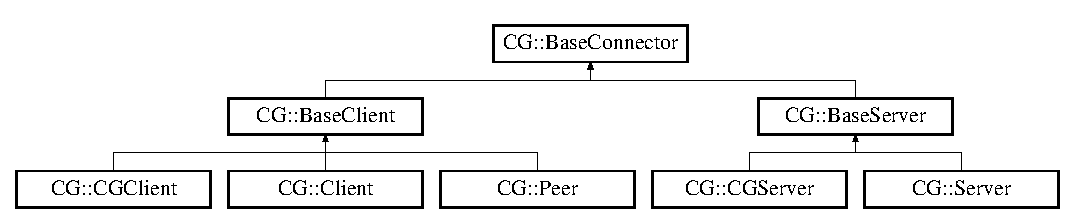
\includegraphics[height=2.564885cm]{class_c_g_1_1_base_connector}
\end{center}
\end{figure}
\subsection*{Public Member Functions}
\begin{DoxyCompactItemize}
\item 
void \mbox{\hyperlink{class_c_g_1_1_base_connector_a16247e8292b28ba8a3017d86dfc30d15}{start}} (\mbox{\hyperlink{class_c_g_1_1_connect_config}{Connect\+Config}} $\ast$config)
\begin{DoxyCompactList}\small\item\em This is a base class to make child class that can use developers. \end{DoxyCompactList}\item 
void \mbox{\hyperlink{class_c_g_1_1_base_connector_abd3e4f816a311c41418d5e090de2de15}{stop}} ()
\begin{DoxyCompactList}\small\item\em stop all action (listen, connect... etc) \end{DoxyCompactList}\item 
virtual int \mbox{\hyperlink{class_c_g_1_1_base_connector_adf8eae41d668ead0f14e7f86b3cea825}{process\+Data}} (\mbox{\hyperlink{class_c_g_1_1_connector_info}{Connector\+Info}} $\ast$\mbox{\hyperlink{class_c_g_1_1_base_connector_ae68321ba56404549f2e655238035ed8d}{connector\+Info}}, char $\ast$data, int data\+Size)=0
\begin{DoxyCompactList}\small\item\em network call this function when came receiving data from others \end{DoxyCompactList}\item 
\mbox{\Hypertarget{class_c_g_1_1_base_connector_a92b1055389fbe5720d6671c29b80b110}\label{class_c_g_1_1_base_connector_a92b1055389fbe5720d6671c29b80b110}} 
Connector\+Type {\bfseries get\+Connector\+Type} ()
\end{DoxyCompactItemize}
\subsection*{Public Attributes}
\begin{DoxyCompactItemize}
\item 
std\+::function$<$ void(Host\+Id)$>$ \mbox{\hyperlink{class_c_g_1_1_base_connector_a458c5e8376f9961d03a37624ad8f3ed6}{on\+Connect}}
\begin{DoxyCompactList}\small\item\em execute function when came requesting connection \end{DoxyCompactList}\item 
std\+::function$<$ void(Host\+Id)$>$ \mbox{\hyperlink{class_c_g_1_1_base_connector_ac33259324e8654e0e89762a723fddbb0}{on\+Disconnect}}
\begin{DoxyCompactList}\small\item\em execute function when came requesting disconnection \end{DoxyCompactList}\end{DoxyCompactItemize}
\subsection*{Protected Attributes}
\begin{DoxyCompactItemize}
\item 
\mbox{\Hypertarget{class_c_g_1_1_base_connector_a58b97c8c461511d26d9305c5d09c2816}\label{class_c_g_1_1_base_connector_a58b97c8c461511d26d9305c5d09c2816}} 
Connector\+Type {\bfseries type}
\item 
\mbox{\Hypertarget{class_c_g_1_1_base_connector_ae68321ba56404549f2e655238035ed8d}\label{class_c_g_1_1_base_connector_ae68321ba56404549f2e655238035ed8d}} 
\mbox{\hyperlink{class_c_g_1_1_connector_info}{Connector\+Info}} $\ast$ \mbox{\hyperlink{class_c_g_1_1_base_connector_ae68321ba56404549f2e655238035ed8d}{connector\+Info}}
\begin{DoxyCompactList}\small\item\em own connector info \end{DoxyCompactList}\item 
\mbox{\Hypertarget{class_c_g_1_1_base_connector_af13a9d2d208f81d46dc6d5b9c3b77e33}\label{class_c_g_1_1_base_connector_af13a9d2d208f81d46dc6d5b9c3b77e33}} 
bool \mbox{\hyperlink{class_c_g_1_1_base_connector_af13a9d2d208f81d46dc6d5b9c3b77e33}{is\+Connected}}
\begin{DoxyCompactList}\small\item\em when start success, set true. if not, set false \end{DoxyCompactList}\end{DoxyCompactItemize}
\subsection*{Friends}
\begin{DoxyCompactItemize}
\item 
\mbox{\Hypertarget{class_c_g_1_1_base_connector_a88b59289ffd793fecd040d32e397b1e9}\label{class_c_g_1_1_base_connector_a88b59289ffd793fecd040d32e397b1e9}} 
class {\bfseries Network}
\end{DoxyCompactItemize}


\subsection{Detailed Description}
This is a base class to make child class that can use developers. 

\begin{DoxyAuthor}{Author}
kim yong-\/chan 
\end{DoxyAuthor}
\begin{DoxyDate}{Date}
2018-\/09-\/08 
\end{DoxyDate}


\subsection{Member Function Documentation}
\mbox{\Hypertarget{class_c_g_1_1_base_connector_adf8eae41d668ead0f14e7f86b3cea825}\label{class_c_g_1_1_base_connector_adf8eae41d668ead0f14e7f86b3cea825}} 
\index{C\+G\+::\+Base\+Connector@{C\+G\+::\+Base\+Connector}!process\+Data@{process\+Data}}
\index{process\+Data@{process\+Data}!C\+G\+::\+Base\+Connector@{C\+G\+::\+Base\+Connector}}
\subsubsection{\texorpdfstring{process\+Data()}{processData()}}
{\footnotesize\ttfamily virtual int C\+G\+::\+Base\+Connector\+::process\+Data (\begin{DoxyParamCaption}\item[{\mbox{\hyperlink{class_c_g_1_1_connector_info}{Connector\+Info}} $\ast$}]{connector\+Info,  }\item[{char $\ast$}]{data,  }\item[{int}]{data\+Size }\end{DoxyParamCaption})\hspace{0.3cm}{\ttfamily [pure virtual]}}



network call this function when came receiving data from others 

\begin{DoxyAuthor}{Author}
kim yong-\/chan 
\end{DoxyAuthor}
\begin{DoxyDate}{Date}
2018-\/09-\/08 
\end{DoxyDate}

\begin{DoxyParams}{Parameters}
{\em Connector\+Info$\ast$} & connector\+Info \+: infomation who send data \\
\hline
{\em char$\ast$} & data \+: receive data from other \\
\hline
{\em int} & data\+Size \+: receive data size \\
\hline
\end{DoxyParams}
\begin{DoxyReturn}{Returns}
int index \+: if data doesn\textquotesingle{}t come all, return 0. if data is not correct, return nagative number. if data come perfect, return data size 
\end{DoxyReturn}


Implemented in \mbox{\hyperlink{class_c_g_1_1_c_g_server_a12598a365b61be0b9d7169a7d1aded49}{C\+G\+::\+C\+G\+Server}}, \mbox{\hyperlink{class_c_g_1_1_c_g_client_a88087f4fdc6e07c8a252d9abe67d9f8b}{C\+G\+::\+C\+G\+Client}}, \mbox{\hyperlink{class_c_g_1_1_server_a846ff65e508699775c54a81091ec76a3}{C\+G\+::\+Server}}, and \mbox{\hyperlink{class_c_g_1_1_client_ad56b8a63eea5c2fea2a0b254758468dd}{C\+G\+::\+Client}}.

\mbox{\Hypertarget{class_c_g_1_1_base_connector_a16247e8292b28ba8a3017d86dfc30d15}\label{class_c_g_1_1_base_connector_a16247e8292b28ba8a3017d86dfc30d15}} 
\index{C\+G\+::\+Base\+Connector@{C\+G\+::\+Base\+Connector}!start@{start}}
\index{start@{start}!C\+G\+::\+Base\+Connector@{C\+G\+::\+Base\+Connector}}
\subsubsection{\texorpdfstring{start()}{start()}}
{\footnotesize\ttfamily void C\+G\+::\+Base\+Connector\+::start (\begin{DoxyParamCaption}\item[{\mbox{\hyperlink{class_c_g_1_1_connect_config}{Connect\+Config}} $\ast$}]{config }\end{DoxyParamCaption})}



This is a base class to make child class that can use developers. 

\begin{DoxyAuthor}{Author}
kim yong-\/chan 
\end{DoxyAuthor}
\begin{DoxyDate}{Date}
2018-\/09-\/08 
\end{DoxyDate}

\begin{DoxyParams}{Parameters}
{\em \mbox{\hyperlink{class_c_g_1_1_connect_config}{Connect\+Config}}} & set ip, port \\
\hline
\end{DoxyParams}
\mbox{\Hypertarget{class_c_g_1_1_base_connector_abd3e4f816a311c41418d5e090de2de15}\label{class_c_g_1_1_base_connector_abd3e4f816a311c41418d5e090de2de15}} 
\index{C\+G\+::\+Base\+Connector@{C\+G\+::\+Base\+Connector}!stop@{stop}}
\index{stop@{stop}!C\+G\+::\+Base\+Connector@{C\+G\+::\+Base\+Connector}}
\subsubsection{\texorpdfstring{stop()}{stop()}}
{\footnotesize\ttfamily void C\+G\+::\+Base\+Connector\+::stop (\begin{DoxyParamCaption}{ }\end{DoxyParamCaption})}



stop all action (listen, connect... etc) 

\begin{DoxyAuthor}{Author}
kim yong-\/chan 
\end{DoxyAuthor}
\begin{DoxyDate}{Date}
2018-\/09-\/08 
\end{DoxyDate}
\begin{DoxyRefDesc}{Todo}
\item[\mbox{\hyperlink{todo__todo000003}{Todo}}]clean memory \end{DoxyRefDesc}


\subsection{Member Data Documentation}
\mbox{\Hypertarget{class_c_g_1_1_base_connector_a458c5e8376f9961d03a37624ad8f3ed6}\label{class_c_g_1_1_base_connector_a458c5e8376f9961d03a37624ad8f3ed6}} 
\index{C\+G\+::\+Base\+Connector@{C\+G\+::\+Base\+Connector}!on\+Connect@{on\+Connect}}
\index{on\+Connect@{on\+Connect}!C\+G\+::\+Base\+Connector@{C\+G\+::\+Base\+Connector}}
\subsubsection{\texorpdfstring{on\+Connect}{onConnect}}
{\footnotesize\ttfamily std\+::function$<$void(Host\+Id)$>$ C\+G\+::\+Base\+Connector\+::on\+Connect}



execute function when came requesting connection 

\begin{DoxyAuthor}{Author}
kim yong-\/chan 
\end{DoxyAuthor}
\begin{DoxyDate}{Date}
2018-\/09-\/08 
\end{DoxyDate}
\mbox{\Hypertarget{class_c_g_1_1_base_connector_ac33259324e8654e0e89762a723fddbb0}\label{class_c_g_1_1_base_connector_ac33259324e8654e0e89762a723fddbb0}} 
\index{C\+G\+::\+Base\+Connector@{C\+G\+::\+Base\+Connector}!on\+Disconnect@{on\+Disconnect}}
\index{on\+Disconnect@{on\+Disconnect}!C\+G\+::\+Base\+Connector@{C\+G\+::\+Base\+Connector}}
\subsubsection{\texorpdfstring{on\+Disconnect}{onDisconnect}}
{\footnotesize\ttfamily std\+::function$<$void(Host\+Id)$>$ C\+G\+::\+Base\+Connector\+::on\+Disconnect}



execute function when came requesting disconnection 

\begin{DoxyAuthor}{Author}
kim yong-\/chan 
\end{DoxyAuthor}
\begin{DoxyDate}{Date}
2018-\/09-\/08 
\end{DoxyDate}


The documentation for this class was generated from the following files\+:\begin{DoxyCompactItemize}
\item 
network/core/Base\+Connector.\+h\item 
network/core/Base\+Connector.\+cpp\end{DoxyCompactItemize}

\hypertarget{class_util_1_1_base_serialize}{}\section{Util\+:\+:Base\+Serialize Class Reference}
\label{class_util_1_1_base_serialize}\index{Util\+::\+Base\+Serialize@{Util\+::\+Base\+Serialize}}


test  




{\ttfamily \#include $<$Serialize.\+h$>$}

Inheritance diagram for Util\+:\+:Base\+Serialize\+:\begin{figure}[H]
\begin{center}
\leavevmode
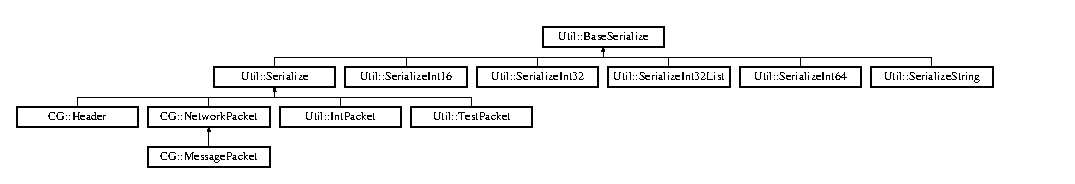
\includegraphics[height=2.028986cm]{class_util_1_1_base_serialize}
\end{center}
\end{figure}
\subsection*{Public Member Functions}
\begin{DoxyCompactItemize}
\item 
virtual int \mbox{\hyperlink{class_util_1_1_base_serialize_ad85061a66f46acebc8457b88d971e022}{serialize}} (char $\ast$data)=0
\begin{DoxyCompactList}\small\item\em �޼��� ���� ���� \end{DoxyCompactList}\item 
\mbox{\Hypertarget{class_util_1_1_base_serialize_af1c7f401a946d0c21a6bca950d5bbe24}\label{class_util_1_1_base_serialize_af1c7f401a946d0c21a6bca950d5bbe24}} 
virtual int {\bfseries deserialize} (const char $\ast$data)=0
\item 
\mbox{\Hypertarget{class_util_1_1_base_serialize_a1b58f2a8b3145c4fd7da86a90d65ba83}\label{class_util_1_1_base_serialize_a1b58f2a8b3145c4fd7da86a90d65ba83}} 
virtual int {\bfseries size} ()=0
\end{DoxyCompactItemize}


\subsection{Detailed Description}
test 

test. 

\subsection{Member Function Documentation}
\mbox{\Hypertarget{class_util_1_1_base_serialize_ad85061a66f46acebc8457b88d971e022}\label{class_util_1_1_base_serialize_ad85061a66f46acebc8457b88d971e022}} 
\index{Util\+::\+Base\+Serialize@{Util\+::\+Base\+Serialize}!serialize@{serialize}}
\index{serialize@{serialize}!Util\+::\+Base\+Serialize@{Util\+::\+Base\+Serialize}}
\subsubsection{\texorpdfstring{serialize()}{serialize()}}
{\footnotesize\ttfamily virtual int Util\+::\+Base\+Serialize\+::serialize (\begin{DoxyParamCaption}\item[{char $\ast$}]{data }\end{DoxyParamCaption})\hspace{0.3cm}{\ttfamily [pure virtual]}}



�޼��� ���� ���� 


\begin{DoxyParams}{Parameters}
{\em string} & a �Ķ���� �� \\
\hline
{\em string} & b \\
\hline
\end{DoxyParams}
\begin{DoxyReturn}{Returns}
mixed$\vert$boolean 
\end{DoxyReturn}


Implemented in \mbox{\hyperlink{class_util_1_1_serialize_ae845c43beb63dddca9cf9fd26b39985d}{Util\+::\+Serialize}}, \mbox{\hyperlink{class_util_1_1_serialize_int32_list_a483adaa0778302e7a3ba86a3e7d23618}{Util\+::\+Serialize\+Int32\+List}}, \mbox{\hyperlink{class_util_1_1_serialize_string_addaa66b71207e6e71a199ffbd0b0998f}{Util\+::\+Serialize\+String}}, \mbox{\hyperlink{class_util_1_1_serialize_int64_ad25b7294bd4ef93ab71377f508534413}{Util\+::\+Serialize\+Int64}}, \mbox{\hyperlink{class_util_1_1_serialize_int32_ae0472419db7afe580206f8498d99c447}{Util\+::\+Serialize\+Int32}}, and \mbox{\hyperlink{class_util_1_1_serialize_int16_aee385ff01c25dbaf72c5da98d8dbc229}{Util\+::\+Serialize\+Int16}}.



The documentation for this class was generated from the following file\+:\begin{DoxyCompactItemize}
\item 
util/serialize/Serialize.\+h\end{DoxyCompactItemize}

\hypertarget{class_c_g_1_1_base_server}{}\section{CG\+:\+:Base\+Server Class Reference}
\label{class_c_g_1_1_base_server}\index{C\+G\+::\+Base\+Server@{C\+G\+::\+Base\+Server}}


This is a base class to make child server class that can use developers.  




{\ttfamily \#include $<$Base\+Server.\+h$>$}

Inheritance diagram for CG\+:\+:Base\+Server\+:\begin{figure}[H]
\begin{center}
\leavevmode
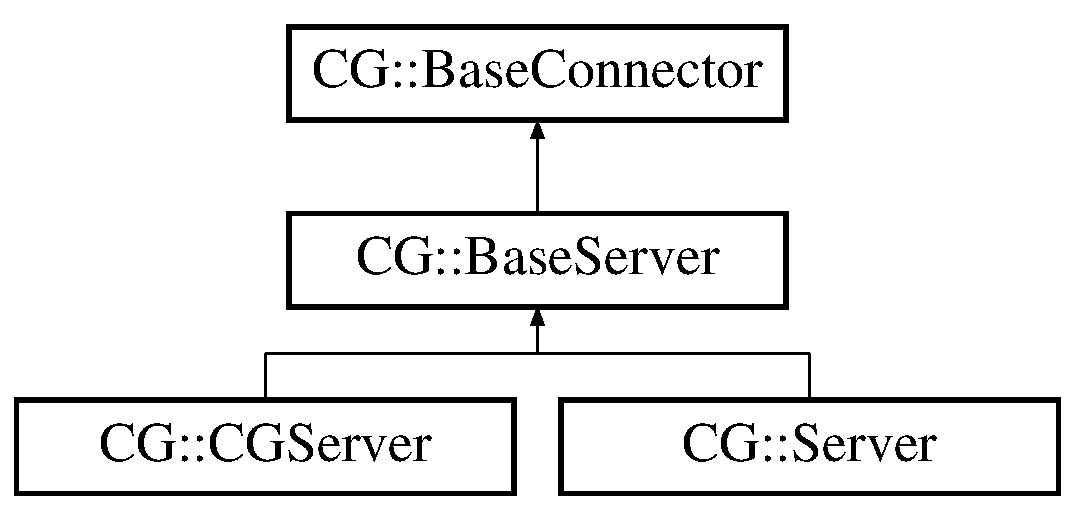
\includegraphics[height=3.000000cm]{class_c_g_1_1_base_server}
\end{center}
\end{figure}
\subsection*{Protected Member Functions}
\begin{DoxyCompactItemize}
\item 
\mbox{\Hypertarget{class_c_g_1_1_base_server_acef9aec3b6c194d413802218597737c0}\label{class_c_g_1_1_base_server_acef9aec3b6c194d413802218597737c0}} 
\mbox{\hyperlink{class_c_g_1_1_base_server_acef9aec3b6c194d413802218597737c0}{Base\+Server}} ()
\begin{DoxyCompactList}\small\item\em set server-\/type \end{DoxyCompactList}\end{DoxyCompactItemize}
\subsection*{Protected Attributes}
\begin{DoxyCompactItemize}
\item 
std\+::map$<$ Host\+Id, \mbox{\hyperlink{class_c_g_1_1_connector_info}{Connector\+Info}} $\ast$ $>$ \mbox{\hyperlink{class_c_g_1_1_base_server_a873e8a48776e1545c06b3dc0e20bdeda}{connector\+Info\+Map}}
\begin{DoxyCompactList}\small\item\em link with client who came from this listener \end{DoxyCompactList}\end{DoxyCompactItemize}
\subsection*{Friends}
\begin{DoxyCompactItemize}
\item 
\mbox{\Hypertarget{class_c_g_1_1_base_server_a88b59289ffd793fecd040d32e397b1e9}\label{class_c_g_1_1_base_server_a88b59289ffd793fecd040d32e397b1e9}} 
class {\bfseries Network}
\end{DoxyCompactItemize}
\subsection*{Additional Inherited Members}


\subsection{Detailed Description}
This is a base class to make child server class that can use developers. 

\begin{DoxyAuthor}{Author}
kim yong-\/chan 
\end{DoxyAuthor}
\begin{DoxyDate}{Date}
2018-\/09-\/08 
\end{DoxyDate}


\subsection{Member Data Documentation}
\mbox{\Hypertarget{class_c_g_1_1_base_server_a873e8a48776e1545c06b3dc0e20bdeda}\label{class_c_g_1_1_base_server_a873e8a48776e1545c06b3dc0e20bdeda}} 
\index{C\+G\+::\+Base\+Server@{C\+G\+::\+Base\+Server}!connector\+Info\+Map@{connector\+Info\+Map}}
\index{connector\+Info\+Map@{connector\+Info\+Map}!C\+G\+::\+Base\+Server@{C\+G\+::\+Base\+Server}}
\subsubsection{\texorpdfstring{connector\+Info\+Map}{connectorInfoMap}}
{\footnotesize\ttfamily std\+::map$<$Host\+Id, \mbox{\hyperlink{class_c_g_1_1_connector_info}{Connector\+Info}}$\ast$$>$ C\+G\+::\+Base\+Server\+::connector\+Info\+Map\hspace{0.3cm}{\ttfamily [protected]}}



link with client who came from this listener 

\begin{DoxyAuthor}{Author}
kim yong-\/chan 
\end{DoxyAuthor}
\begin{DoxyDate}{Date}
2018-\/09-\/08 
\end{DoxyDate}


The documentation for this class was generated from the following file\+:\begin{DoxyCompactItemize}
\item 
network/core/Base\+Server.\+h\end{DoxyCompactItemize}

\hypertarget{class_util_1_1_b_queue}{}\section{Util\+:\+:B\+Queue$<$ T $>$ Class Template Reference}
\label{class_util_1_1_b_queue}\index{Util\+::\+B\+Queue$<$ T $>$@{Util\+::\+B\+Queue$<$ T $>$}}
Inheritance diagram for Util\+:\+:B\+Queue$<$ T $>$\+:\begin{figure}[H]
\begin{center}
\leavevmode
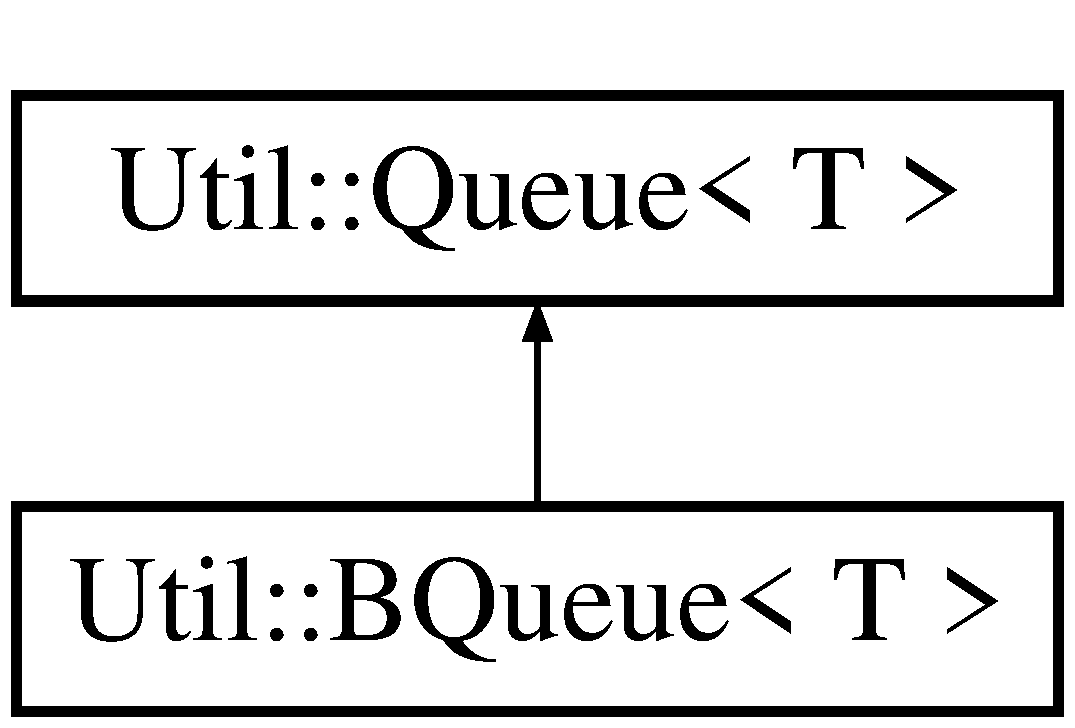
\includegraphics[height=2.000000cm]{class_util_1_1_b_queue}
\end{center}
\end{figure}
\subsection*{Public Member Functions}
\begin{DoxyCompactItemize}
\item 
\mbox{\Hypertarget{class_util_1_1_b_queue_a88111ecf359f17086671177a5793c174}\label{class_util_1_1_b_queue_a88111ecf359f17086671177a5793c174}} 
T {\bfseries pop} ()
\item 
\mbox{\Hypertarget{class_util_1_1_b_queue_a67606aeb3c886c920f932a144368f052}\label{class_util_1_1_b_queue_a67606aeb3c886c920f932a144368f052}} 
void {\bfseries push} (T t)
\item 
\mbox{\Hypertarget{class_util_1_1_b_queue_a9fd764eed02729fdb1eada4142df5dd3}\label{class_util_1_1_b_queue_a9fd764eed02729fdb1eada4142df5dd3}} 
int {\bfseries size} ()
\end{DoxyCompactItemize}
\subsection*{Public Attributes}
\begin{DoxyCompactItemize}
\item 
\mbox{\Hypertarget{class_util_1_1_b_queue_a65a8a52af6c65ccb6fa96e32dc05437c}\label{class_util_1_1_b_queue_a65a8a52af6c65ccb6fa96e32dc05437c}} 
std\+::queue$<$ T $>$ {\bfseries object\+Queue}
\item 
\mbox{\Hypertarget{class_util_1_1_b_queue_ae58ea571bd773a6dbcc920d087021902}\label{class_util_1_1_b_queue_ae58ea571bd773a6dbcc920d087021902}} 
std\+::mutex {\bfseries mutex}
\item 
\mbox{\Hypertarget{class_util_1_1_b_queue_afe3a34e631859753f7ba74627cf0c578}\label{class_util_1_1_b_queue_afe3a34e631859753f7ba74627cf0c578}} 
std\+::condition\+\_\+variable {\bfseries cv}
\end{DoxyCompactItemize}


The documentation for this class was generated from the following file\+:\begin{DoxyCompactItemize}
\item 
util/queue/B\+Queue.\+h\end{DoxyCompactItemize}

\hypertarget{class_c_g_1_1_buffer}{}\section{CG\+:\+:Buffer Class Reference}
\label{class_c_g_1_1_buffer}\index{C\+G\+::\+Buffer@{C\+G\+::\+Buffer}}


buffer that move receive data, storage non-\/finished data  




{\ttfamily \#include $<$Buffer.\+h$>$}

\subsection*{Public Member Functions}
\begin{DoxyCompactItemize}
\item 
\mbox{\Hypertarget{class_c_g_1_1_buffer_a1e06b035a494ef3788bffe96a97e19eb}\label{class_c_g_1_1_buffer_a1e06b035a494ef3788bffe96a97e19eb}} 
void \mbox{\hyperlink{class_c_g_1_1_buffer_a1e06b035a494ef3788bffe96a97e19eb}{reset}} ()
\begin{DoxyCompactList}\small\item\em reset buffer \end{DoxyCompactList}\end{DoxyCompactItemize}
\subsection*{Public Attributes}
\begin{DoxyCompactItemize}
\item 
\mbox{\Hypertarget{class_c_g_1_1_buffer_a83f061df0766efbb8c8dd18ec663a021}\label{class_c_g_1_1_buffer_a83f061df0766efbb8c8dd18ec663a021}} 
char \mbox{\hyperlink{class_c_g_1_1_buffer_a83f061df0766efbb8c8dd18ec663a021}{data}} \mbox{[}R\+C\+V\+\_\+\+B\+UF\mbox{]}
\begin{DoxyCompactList}\small\item\em data in buffer \end{DoxyCompactList}\item 
\mbox{\Hypertarget{class_c_g_1_1_buffer_a6db7caf87fb31fcfabbf96eca2b3016c}\label{class_c_g_1_1_buffer_a6db7caf87fb31fcfabbf96eca2b3016c}} 
int \mbox{\hyperlink{class_c_g_1_1_buffer_a6db7caf87fb31fcfabbf96eca2b3016c}{start\+Index}}
\begin{DoxyCompactList}\small\item\em data start index \end{DoxyCompactList}\item 
\mbox{\Hypertarget{class_c_g_1_1_buffer_a037dfe4011fff334709dd66e8809a8b5}\label{class_c_g_1_1_buffer_a037dfe4011fff334709dd66e8809a8b5}} 
int \mbox{\hyperlink{class_c_g_1_1_buffer_a037dfe4011fff334709dd66e8809a8b5}{data\+Size}}
\begin{DoxyCompactList}\small\item\em data size \end{DoxyCompactList}\end{DoxyCompactItemize}


\subsection{Detailed Description}
buffer that move receive data, storage non-\/finished data 

\begin{DoxyAuthor}{Author}
kim yong-\/chan 
\end{DoxyAuthor}
\begin{DoxyDate}{Date}
2018-\/09-\/08 
\end{DoxyDate}


The documentation for this class was generated from the following file\+:\begin{DoxyCompactItemize}
\item 
network/core/Buffer.\+h\end{DoxyCompactItemize}

\hypertarget{class_c_g_1_1_c_g_client}{}\section{CG\+:\+:C\+G\+Client Class Reference}
\label{class_c_g_1_1_c_g_client}\index{C\+G\+::\+C\+G\+Client@{C\+G\+::\+C\+G\+Client}}
Inheritance diagram for CG\+:\+:C\+G\+Client\+:\begin{figure}[H]
\begin{center}
\leavevmode
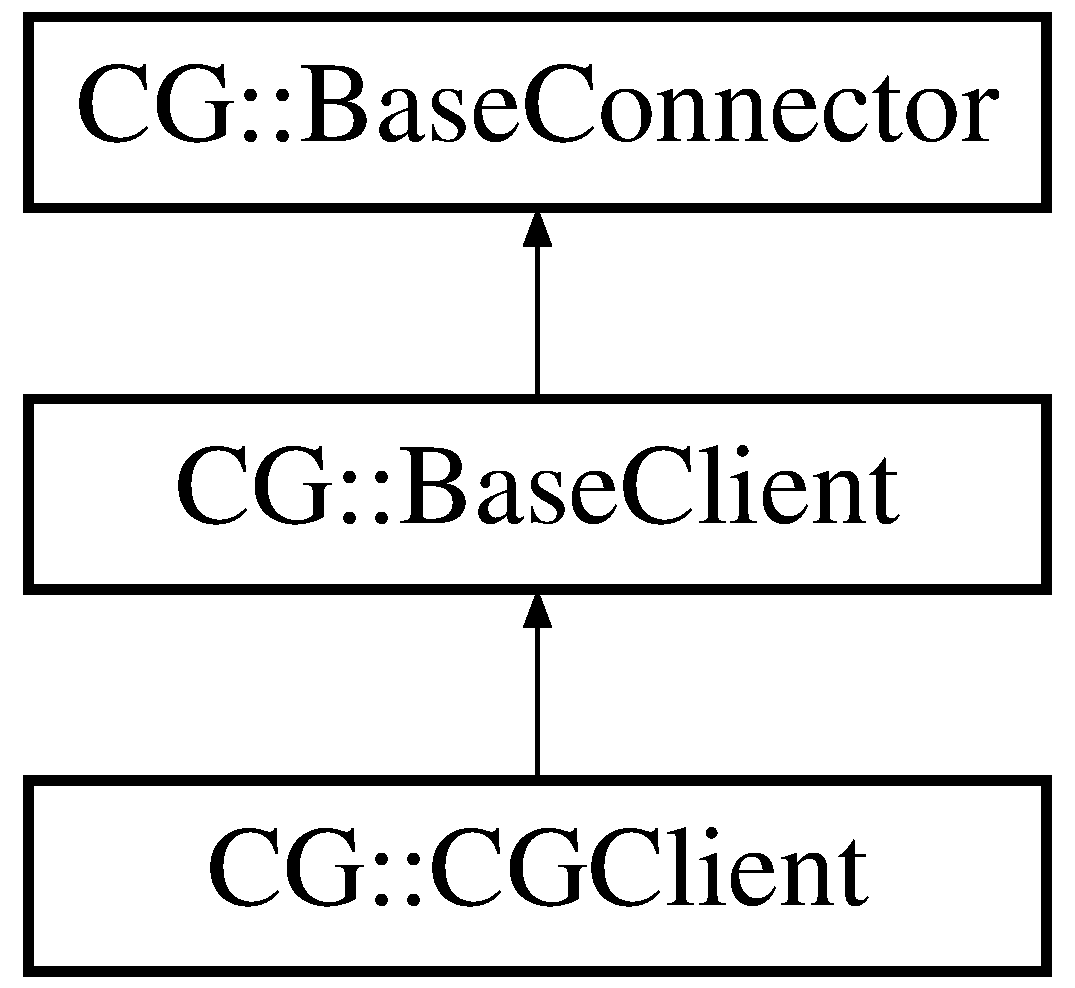
\includegraphics[height=3.000000cm]{class_c_g_1_1_c_g_client}
\end{center}
\end{figure}
\subsection*{Public Member Functions}
\begin{DoxyCompactItemize}
\item 
\mbox{\Hypertarget{class_c_g_1_1_c_g_client_a30a46e32bff3f67e1c7c23b70ca39963}\label{class_c_g_1_1_c_g_client_a30a46e32bff3f67e1c7c23b70ca39963}} 
{\footnotesize template$<$typename T , typename std\+::enable\+\_\+if$<$ std\+::is\+\_\+base\+\_\+of$<$ C\+G\+::\+Network\+Packet, T $>$\+::value $>$\+::type $\ast$  = nullptr$>$ }\\void {\bfseries register\+Packet} (std\+::function$<$ void(Host\+Id, \mbox{\hyperlink{class_c_g_1_1_network_packet}{Network\+Packet}} $\ast$)$>$ on\+Receive\+N\+Packet)
\item 
int \mbox{\hyperlink{class_c_g_1_1_c_g_client_a88087f4fdc6e07c8a252d9abe67d9f8b}{process\+Data}} (\mbox{\hyperlink{class_c_g_1_1_connector_info}{Connector\+Info}} $\ast$\mbox{\hyperlink{class_c_g_1_1_base_connector_ae68321ba56404549f2e655238035ed8d}{connector\+Info}}, char $\ast$data, int data\+Size)
\begin{DoxyCompactList}\small\item\em network call this function when came receiving data from others \end{DoxyCompactList}\item 
\mbox{\Hypertarget{class_c_g_1_1_c_g_client_a6a550e4c1d5143655d54e4acece405f2}\label{class_c_g_1_1_c_g_client_a6a550e4c1d5143655d54e4acece405f2}} 
void {\bfseries send\+Packet} (\mbox{\hyperlink{class_c_g_1_1_network_packet}{Network\+Packet}} $\ast$packet)
\end{DoxyCompactItemize}
\subsection*{Public Attributes}
\begin{DoxyCompactItemize}
\item 
\mbox{\Hypertarget{class_c_g_1_1_c_g_client_ab3946b15ed83de702a29a7b16de2c9de}\label{class_c_g_1_1_c_g_client_ab3946b15ed83de702a29a7b16de2c9de}} 
\mbox{\hyperlink{class_c_g_1_1_c_g_network_handler}{C\+G\+Network\+Handler}} $\ast$ {\bfseries network\+Handler}
\end{DoxyCompactItemize}
\subsection*{Additional Inherited Members}


\subsection{Member Function Documentation}
\mbox{\Hypertarget{class_c_g_1_1_c_g_client_a88087f4fdc6e07c8a252d9abe67d9f8b}\label{class_c_g_1_1_c_g_client_a88087f4fdc6e07c8a252d9abe67d9f8b}} 
\index{C\+G\+::\+C\+G\+Client@{C\+G\+::\+C\+G\+Client}!process\+Data@{process\+Data}}
\index{process\+Data@{process\+Data}!C\+G\+::\+C\+G\+Client@{C\+G\+::\+C\+G\+Client}}
\subsubsection{\texorpdfstring{process\+Data()}{processData()}}
{\footnotesize\ttfamily int C\+G\+::\+C\+G\+Client\+::process\+Data (\begin{DoxyParamCaption}\item[{\mbox{\hyperlink{class_c_g_1_1_connector_info}{Connector\+Info}} $\ast$}]{connector\+Info,  }\item[{char $\ast$}]{data,  }\item[{int}]{data\+Size }\end{DoxyParamCaption})\hspace{0.3cm}{\ttfamily [virtual]}}



network call this function when came receiving data from others 

\begin{DoxyAuthor}{Author}
kim yong-\/chan 
\end{DoxyAuthor}
\begin{DoxyDate}{Date}
2018-\/09-\/08 
\end{DoxyDate}

\begin{DoxyParams}{Parameters}
{\em Connector\+Info$\ast$} & connector\+Info \+: infomation who send data \\
\hline
{\em char$\ast$} & data \+: receive data from other \\
\hline
{\em int} & data\+Size \+: receive data size \\
\hline
\end{DoxyParams}
\begin{DoxyReturn}{Returns}
int index \+: if data doesn\textquotesingle{}t come all, return 0. if data is not correct, return nagative number. if data come perfect, return data size 
\end{DoxyReturn}


Implements \mbox{\hyperlink{class_c_g_1_1_base_connector_adf8eae41d668ead0f14e7f86b3cea825}{C\+G\+::\+Base\+Connector}}.



The documentation for this class was generated from the following files\+:\begin{DoxyCompactItemize}
\item 
network/module/packet/C\+G\+Client.\+h\item 
network/module/packet/C\+G\+Client.\+cpp\end{DoxyCompactItemize}

\hypertarget{class_c_g_1_1_c_g_file_parser}{}\section{CG\+:\+:C\+G\+File\+Parser Class Reference}
\label{class_c_g_1_1_c_g_file_parser}\index{C\+G\+::\+C\+G\+File\+Parser@{C\+G\+::\+C\+G\+File\+Parser}}


convert file to use in cpp source  




{\ttfamily \#include $<$C\+G\+File\+Parser.\+h$>$}

\subsection*{Public Member Functions}
\begin{DoxyCompactItemize}
\item 
std\+::unordered\+\_\+map$<$ std\+::string, std\+::string $>$ \mbox{\hyperlink{class_c_g_1_1_c_g_file_parser_a527706748bc55bf13819682a5e82d8b2}{parse\+Setting\+File}} (const char $\ast$file)
\begin{DoxyCompactList}\small\item\em get file and convert to key/value \end{DoxyCompactList}\end{DoxyCompactItemize}


\subsection{Detailed Description}
convert file to use in cpp source 

\begin{DoxyAuthor}{Author}
kim yong-\/chan 
\end{DoxyAuthor}
\begin{DoxyDate}{Date}
2018-\/09-\/08 
\end{DoxyDate}


\subsection{Member Function Documentation}
\mbox{\Hypertarget{class_c_g_1_1_c_g_file_parser_a527706748bc55bf13819682a5e82d8b2}\label{class_c_g_1_1_c_g_file_parser_a527706748bc55bf13819682a5e82d8b2}} 
\index{C\+G\+::\+C\+G\+File\+Parser@{C\+G\+::\+C\+G\+File\+Parser}!parse\+Setting\+File@{parse\+Setting\+File}}
\index{parse\+Setting\+File@{parse\+Setting\+File}!C\+G\+::\+C\+G\+File\+Parser@{C\+G\+::\+C\+G\+File\+Parser}}
\subsubsection{\texorpdfstring{parse\+Setting\+File()}{parseSettingFile()}}
{\footnotesize\ttfamily std\+::unordered\+\_\+map$<$ std\+::string, std\+::string $>$ C\+G\+::\+C\+G\+File\+Parser\+::parse\+Setting\+File (\begin{DoxyParamCaption}\item[{const char $\ast$}]{file }\end{DoxyParamCaption})}



get file and convert to key/value 

\begin{DoxyAuthor}{Author}
kim yong-\/chan 
\end{DoxyAuthor}
\begin{DoxyDate}{Date}
2018-\/09-\/08 
\end{DoxyDate}

\begin{DoxyParams}{Parameters}
{\em const} & char$\ast$ file \+: file path \\
\hline
\end{DoxyParams}
\begin{DoxyReturn}{Returns}
std\+::unordered\+\_\+map$<$std\+::string, std\+::string$>$ \+: return key/value 
\end{DoxyReturn}


The documentation for this class was generated from the following files\+:\begin{DoxyCompactItemize}
\item 
network/core/C\+G\+File\+Parser.\+h\item 
network/core/C\+G\+File\+Parser.\+cpp\end{DoxyCompactItemize}

\hypertarget{class_c_g_1_1_c_g_network_handler}{}\section{CG\+:\+:C\+G\+Network\+Handler Class Reference}
\label{class_c_g_1_1_c_g_network_handler}\index{C\+G\+::\+C\+G\+Network\+Handler@{C\+G\+::\+C\+G\+Network\+Handler}}
\subsection*{Public Member Functions}
\begin{DoxyCompactItemize}
\item 
\mbox{\Hypertarget{class_c_g_1_1_c_g_network_handler_a597cfc31218fb6ee2e06eb626917b0c4}\label{class_c_g_1_1_c_g_network_handler_a597cfc31218fb6ee2e06eb626917b0c4}} 
int {\bfseries process\+Data} (\mbox{\hyperlink{class_c_g_1_1_connector_info}{Connector\+Info}} $\ast$connector\+Info, char $\ast$data, int data\+Size)
\item 
\mbox{\Hypertarget{class_c_g_1_1_c_g_network_handler_a1bcbb6de607fec8664ace5427ae0f911}\label{class_c_g_1_1_c_g_network_handler_a1bcbb6de607fec8664ace5427ae0f911}} 
{\footnotesize template$<$typename T , typename std\+::enable\+\_\+if$<$ std\+::is\+\_\+base\+\_\+of$<$ C\+G\+::\+Network\+Packet, T $>$\+::value $>$\+::type $\ast$  = nullptr$>$ }\\void {\bfseries register\+Packet} (std\+::function$<$ void(Host\+Id, \mbox{\hyperlink{class_c_g_1_1_network_packet}{Network\+Packet}} $\ast$)$>$ on\+Receive\+N\+Packet)
\item 
\mbox{\Hypertarget{class_c_g_1_1_c_g_network_handler_af007aa7b64add10eb269e445db6800d2}\label{class_c_g_1_1_c_g_network_handler_af007aa7b64add10eb269e445db6800d2}} 
void {\bfseries send\+Packet} (Host\+Id host\+Id, \mbox{\hyperlink{class_c_g_1_1_network_packet}{Network\+Packet}} $\ast$packet)
\end{DoxyCompactItemize}
\subsection*{Public Attributes}
\begin{DoxyCompactItemize}
\item 
\mbox{\Hypertarget{class_c_g_1_1_c_g_network_handler_af8c3950b916ed65461534d14185f059d}\label{class_c_g_1_1_c_g_network_handler_af8c3950b916ed65461534d14185f059d}} 
std\+::map$<$ np\+Type\+\_\+t, \mbox{\hyperlink{class_c_g_1_1_packet_function}{Packet\+Function}} $\ast$ $>$ {\bfseries np\+Map}
\item 
\mbox{\Hypertarget{class_c_g_1_1_c_g_network_handler_a146e1a5895d3c91cdef43890fcc65a68}\label{class_c_g_1_1_c_g_network_handler_a146e1a5895d3c91cdef43890fcc65a68}} 
std\+::map$<$ np\+Type\+\_\+t, \mbox{\hyperlink{class_c_g_1_1_packet_function}{Packet\+Function}} $\ast$ $>$\+::iterator {\bfseries itr}
\end{DoxyCompactItemize}
\subsection*{Friends}
\begin{DoxyCompactItemize}
\item 
\mbox{\Hypertarget{class_c_g_1_1_c_g_network_handler_a88b59289ffd793fecd040d32e397b1e9}\label{class_c_g_1_1_c_g_network_handler_a88b59289ffd793fecd040d32e397b1e9}} 
class {\bfseries Network}
\end{DoxyCompactItemize}


The documentation for this class was generated from the following files\+:\begin{DoxyCompactItemize}
\item 
network/module/packet/C\+G\+Network\+Handler.\+h\item 
network/module/packet/C\+G\+Network\+Handler.\+cpp\end{DoxyCompactItemize}

\hypertarget{class_c_g_1_1_c_g_server}{}\section{CG\+:\+:C\+G\+Server Class Reference}
\label{class_c_g_1_1_c_g_server}\index{C\+G\+::\+C\+G\+Server@{C\+G\+::\+C\+G\+Server}}
Inheritance diagram for CG\+:\+:C\+G\+Server\+:\begin{figure}[H]
\begin{center}
\leavevmode
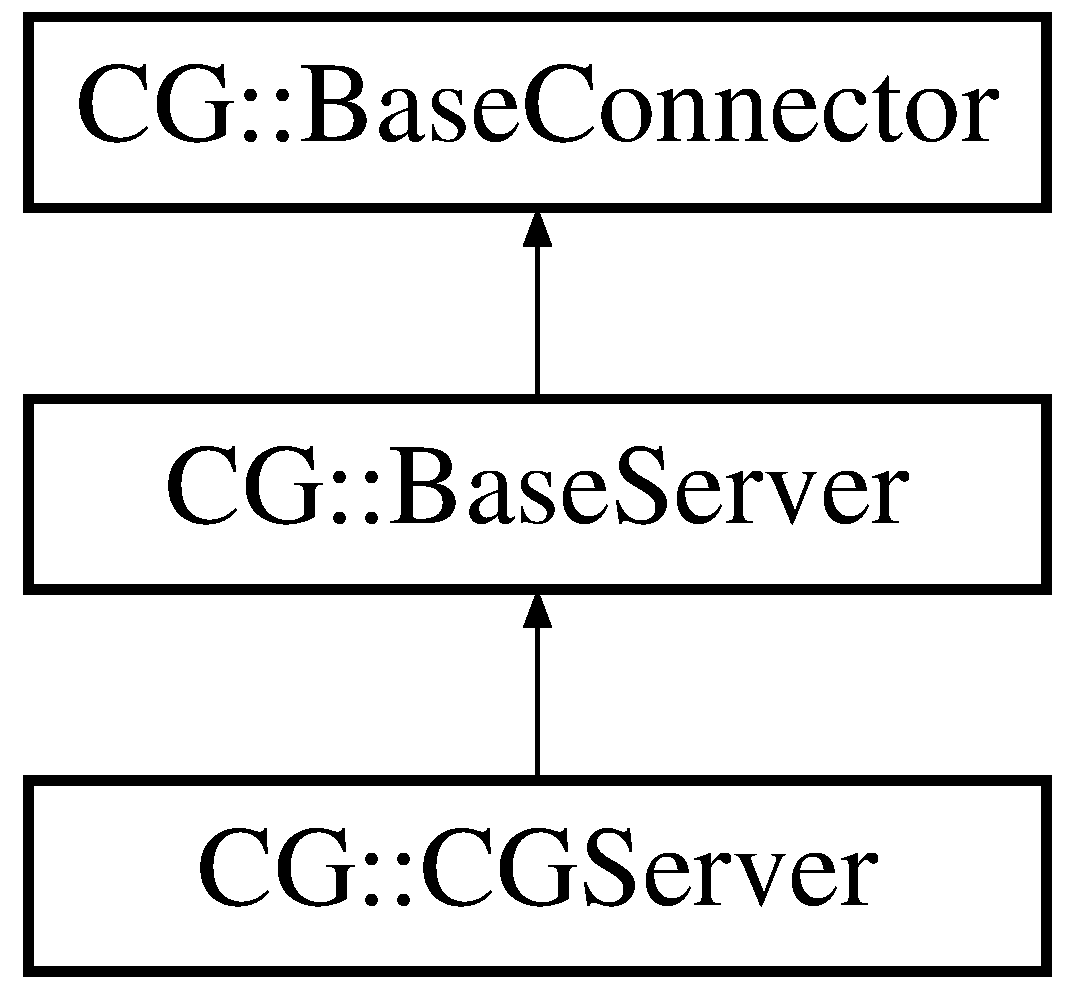
\includegraphics[height=3.000000cm]{class_c_g_1_1_c_g_server}
\end{center}
\end{figure}
\subsection*{Public Member Functions}
\begin{DoxyCompactItemize}
\item 
\mbox{\Hypertarget{class_c_g_1_1_c_g_server_a6ab75a0350236cb0c279dc2a052e13fb}\label{class_c_g_1_1_c_g_server_a6ab75a0350236cb0c279dc2a052e13fb}} 
{\footnotesize template$<$typename T , typename std\+::enable\+\_\+if$<$ std\+::is\+\_\+base\+\_\+of$<$ C\+G\+::\+Network\+Packet, T $>$\+::value $>$\+::type $\ast$  = nullptr$>$ }\\void {\bfseries register\+Packet} (std\+::function$<$ void(Host\+Id, \mbox{\hyperlink{class_c_g_1_1_network_packet}{Network\+Packet}} $\ast$)$>$ on\+Receive\+N\+Packet)
\item 
int \mbox{\hyperlink{class_c_g_1_1_c_g_server_a12598a365b61be0b9d7169a7d1aded49}{process\+Data}} (\mbox{\hyperlink{class_c_g_1_1_connector_info}{Connector\+Info}} $\ast$\mbox{\hyperlink{class_c_g_1_1_base_connector_ae68321ba56404549f2e655238035ed8d}{connector\+Info}}, char $\ast$data, int data\+Size)
\begin{DoxyCompactList}\small\item\em network call this function when came receiving data from others \end{DoxyCompactList}\item 
\mbox{\Hypertarget{class_c_g_1_1_c_g_server_ab7d95f379dde4cbc48acc476e1475d6a}\label{class_c_g_1_1_c_g_server_ab7d95f379dde4cbc48acc476e1475d6a}} 
void {\bfseries send\+Packet} (Host\+Id host\+Id, \mbox{\hyperlink{class_c_g_1_1_network_packet}{Network\+Packet}} $\ast$packet)
\end{DoxyCompactItemize}
\subsection*{Public Attributes}
\begin{DoxyCompactItemize}
\item 
\mbox{\Hypertarget{class_c_g_1_1_c_g_server_a502226ceaa105fa3c3046391ee71742f}\label{class_c_g_1_1_c_g_server_a502226ceaa105fa3c3046391ee71742f}} 
\mbox{\hyperlink{class_c_g_1_1_c_g_network_handler}{C\+G\+Network\+Handler}} $\ast$ {\bfseries network\+Handler}
\end{DoxyCompactItemize}
\subsection*{Additional Inherited Members}


\subsection{Member Function Documentation}
\mbox{\Hypertarget{class_c_g_1_1_c_g_server_a12598a365b61be0b9d7169a7d1aded49}\label{class_c_g_1_1_c_g_server_a12598a365b61be0b9d7169a7d1aded49}} 
\index{C\+G\+::\+C\+G\+Server@{C\+G\+::\+C\+G\+Server}!process\+Data@{process\+Data}}
\index{process\+Data@{process\+Data}!C\+G\+::\+C\+G\+Server@{C\+G\+::\+C\+G\+Server}}
\subsubsection{\texorpdfstring{process\+Data()}{processData()}}
{\footnotesize\ttfamily int C\+G\+::\+C\+G\+Server\+::process\+Data (\begin{DoxyParamCaption}\item[{\mbox{\hyperlink{class_c_g_1_1_connector_info}{Connector\+Info}} $\ast$}]{connector\+Info,  }\item[{char $\ast$}]{data,  }\item[{int}]{data\+Size }\end{DoxyParamCaption})\hspace{0.3cm}{\ttfamily [virtual]}}



network call this function when came receiving data from others 

\begin{DoxyAuthor}{Author}
kim yong-\/chan 
\end{DoxyAuthor}
\begin{DoxyDate}{Date}
2018-\/09-\/08 
\end{DoxyDate}

\begin{DoxyParams}{Parameters}
{\em Connector\+Info$\ast$} & connector\+Info \+: infomation who send data \\
\hline
{\em char$\ast$} & data \+: receive data from other \\
\hline
{\em int} & data\+Size \+: receive data size \\
\hline
\end{DoxyParams}
\begin{DoxyReturn}{Returns}
int index \+: if data doesn\textquotesingle{}t come all, return 0. if data is not correct, return nagative number. if data come perfect, return data size 
\end{DoxyReturn}


Implements \mbox{\hyperlink{class_c_g_1_1_base_connector_adf8eae41d668ead0f14e7f86b3cea825}{C\+G\+::\+Base\+Connector}}.



The documentation for this class was generated from the following files\+:\begin{DoxyCompactItemize}
\item 
network/module/packet/C\+G\+Server.\+h\item 
network/module/packet/C\+G\+Server.\+cpp\end{DoxyCompactItemize}

\hypertarget{class_c_g_1_1_client}{}\section{CG\+:\+:Client Class Reference}
\label{class_c_g_1_1_client}\index{C\+G\+::\+Client@{C\+G\+::\+Client}}
Inheritance diagram for CG\+:\+:Client\+:\begin{figure}[H]
\begin{center}
\leavevmode
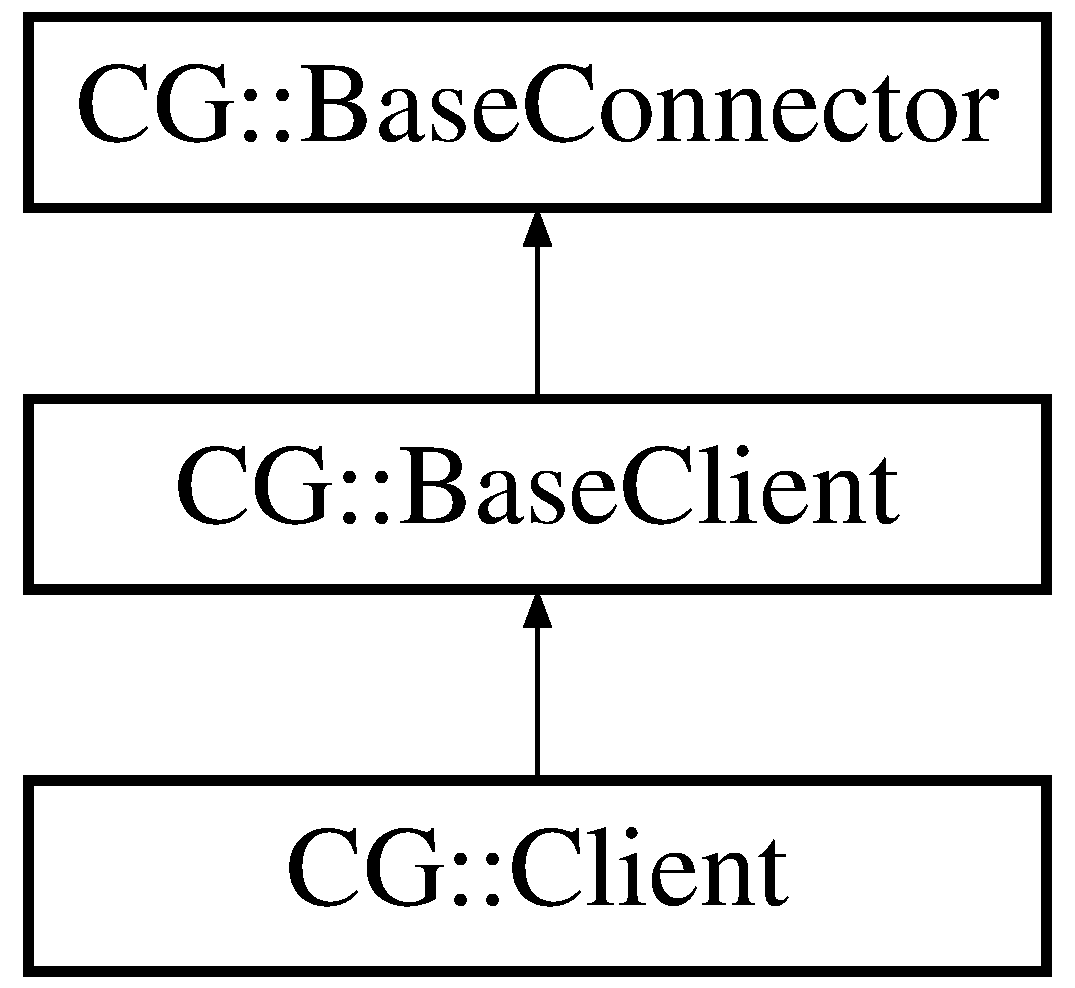
\includegraphics[height=3.000000cm]{class_c_g_1_1_client}
\end{center}
\end{figure}
\subsection*{Public Member Functions}
\begin{DoxyCompactItemize}
\item 
int \mbox{\hyperlink{class_c_g_1_1_client_ad56b8a63eea5c2fea2a0b254758468dd}{process\+Data}} (\mbox{\hyperlink{class_c_g_1_1_connector_info}{Connector\+Info}} $\ast$\mbox{\hyperlink{class_c_g_1_1_base_connector_ae68321ba56404549f2e655238035ed8d}{connector\+Info}}, char $\ast$data, int data\+Size)
\begin{DoxyCompactList}\small\item\em network call this function when came receiving data from others \end{DoxyCompactList}\item 
\mbox{\Hypertarget{class_c_g_1_1_client_a29e0c78ca332fcdbc47db9cd72616fae}\label{class_c_g_1_1_client_a29e0c78ca332fcdbc47db9cd72616fae}} 
void {\bfseries send\+Message} (const char $\ast$data, int data\+Size)
\item 
\mbox{\Hypertarget{class_c_g_1_1_client_a5e84eb047a1a425b1a1abd3291c8a0d1}\label{class_c_g_1_1_client_a5e84eb047a1a425b1a1abd3291c8a0d1}} 
void {\bfseries send\+Message} (std\+::string message)
\end{DoxyCompactItemize}
\subsection*{Public Attributes}
\begin{DoxyCompactItemize}
\item 
\mbox{\Hypertarget{class_c_g_1_1_client_a2c4e42613c4f738c8930b37cf31e864f}\label{class_c_g_1_1_client_a2c4e42613c4f738c8930b37cf31e864f}} 
std\+::function$<$ void(Host\+Id, char $\ast$, int)$>$ {\bfseries on\+Receive}
\item 
\mbox{\Hypertarget{class_c_g_1_1_client_a38410c9c6bb7ce839a3286b785e04cf9}\label{class_c_g_1_1_client_a38410c9c6bb7ce839a3286b785e04cf9}} 
\mbox{\hyperlink{class_c_g_1_1_network_handler}{Network\+Handler}} $\ast$ {\bfseries network\+Handler}
\end{DoxyCompactItemize}
\subsection*{Additional Inherited Members}


\subsection{Member Function Documentation}
\mbox{\Hypertarget{class_c_g_1_1_client_ad56b8a63eea5c2fea2a0b254758468dd}\label{class_c_g_1_1_client_ad56b8a63eea5c2fea2a0b254758468dd}} 
\index{C\+G\+::\+Client@{C\+G\+::\+Client}!process\+Data@{process\+Data}}
\index{process\+Data@{process\+Data}!C\+G\+::\+Client@{C\+G\+::\+Client}}
\subsubsection{\texorpdfstring{process\+Data()}{processData()}}
{\footnotesize\ttfamily int C\+G\+::\+Client\+::process\+Data (\begin{DoxyParamCaption}\item[{\mbox{\hyperlink{class_c_g_1_1_connector_info}{Connector\+Info}} $\ast$}]{connector\+Info,  }\item[{char $\ast$}]{data,  }\item[{int}]{data\+Size }\end{DoxyParamCaption})\hspace{0.3cm}{\ttfamily [virtual]}}



network call this function when came receiving data from others 

\begin{DoxyAuthor}{Author}
kim yong-\/chan 
\end{DoxyAuthor}
\begin{DoxyDate}{Date}
2018-\/09-\/08 
\end{DoxyDate}

\begin{DoxyParams}{Parameters}
{\em Connector\+Info$\ast$} & connector\+Info \+: infomation who send data \\
\hline
{\em char$\ast$} & data \+: receive data from other \\
\hline
{\em int} & data\+Size \+: receive data size \\
\hline
\end{DoxyParams}
\begin{DoxyReturn}{Returns}
int index \+: if data doesn\textquotesingle{}t come all, return 0. if data is not correct, return nagative number. if data come perfect, return data size 
\end{DoxyReturn}


Implements \mbox{\hyperlink{class_c_g_1_1_base_connector_adf8eae41d668ead0f14e7f86b3cea825}{C\+G\+::\+Base\+Connector}}.



The documentation for this class was generated from the following files\+:\begin{DoxyCompactItemize}
\item 
network/module/basic/Client.\+h\item 
network/module/basic/Client.\+cpp\end{DoxyCompactItemize}

\hypertarget{class_c_g_1_1_client_config}{}\section{CG\+:\+:Client\+Config Class Reference}
\label{class_c_g_1_1_client_config}\index{C\+G\+::\+Client\+Config@{C\+G\+::\+Client\+Config}}


it is client config. same with connect\+Config but it will storage additional client infomation later  




{\ttfamily \#include $<$Base\+Client.\+h$>$}

Inheritance diagram for CG\+:\+:Client\+Config\+:\begin{figure}[H]
\begin{center}
\leavevmode
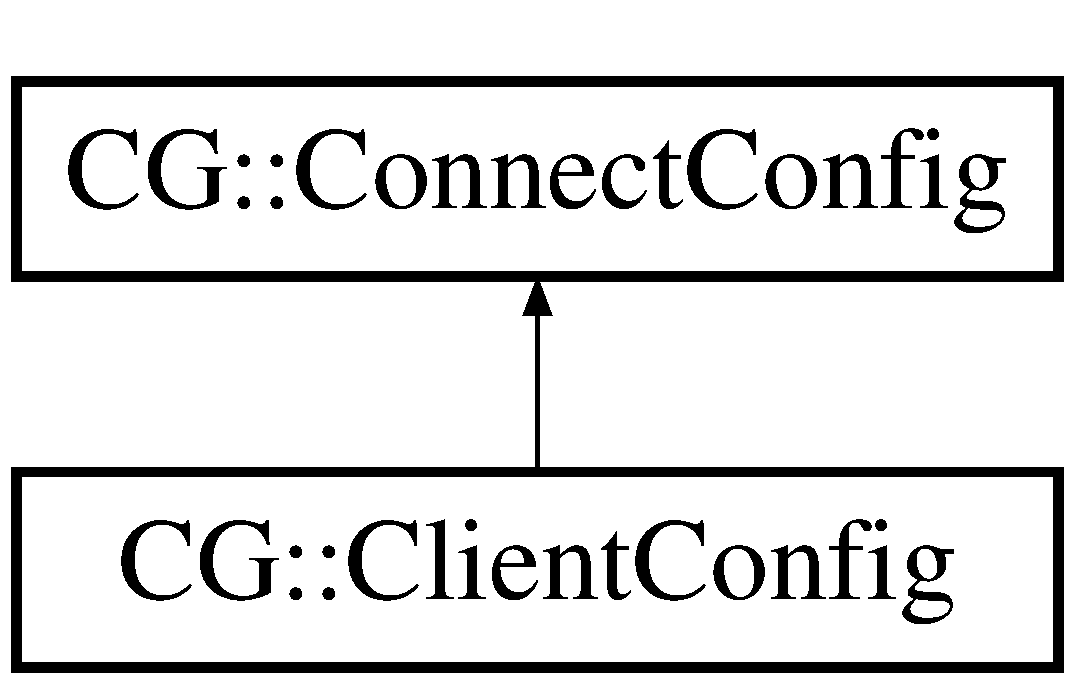
\includegraphics[height=2.000000cm]{class_c_g_1_1_client_config}
\end{center}
\end{figure}
\subsection*{Additional Inherited Members}


\subsection{Detailed Description}
it is client config. same with connect\+Config but it will storage additional client infomation later 

\begin{DoxyAuthor}{Author}
kim yong-\/chan 
\end{DoxyAuthor}
\begin{DoxyDate}{Date}
2018-\/09-\/08 
\end{DoxyDate}


The documentation for this class was generated from the following file\+:\begin{DoxyCompactItemize}
\item 
network/core/Base\+Client.\+h\end{DoxyCompactItemize}

\hypertarget{class_c_g_1_1_connect_config}{}\section{CG\+:\+:Connect\+Config Class Reference}
\label{class_c_g_1_1_connect_config}\index{C\+G\+::\+Connect\+Config@{C\+G\+::\+Connect\+Config}}


Set ip, port to connect with other.  




{\ttfamily \#include $<$Base\+Connector.\+h$>$}

Inheritance diagram for CG\+:\+:Connect\+Config\+:\begin{figure}[H]
\begin{center}
\leavevmode
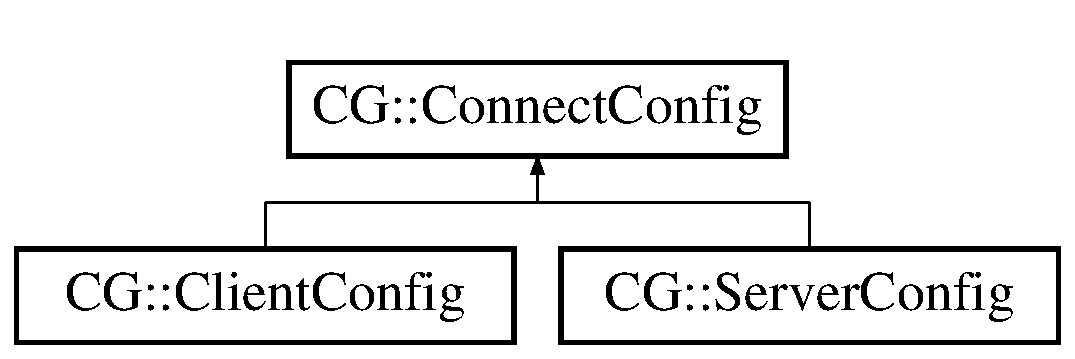
\includegraphics[height=2.000000cm]{class_c_g_1_1_connect_config}
\end{center}
\end{figure}
\subsection*{Public Attributes}
\begin{DoxyCompactItemize}
\item 
\mbox{\Hypertarget{class_c_g_1_1_connect_config_ac8d98bcc93d6e5c968e95a4d4889570a}\label{class_c_g_1_1_connect_config_ac8d98bcc93d6e5c968e95a4d4889570a}} 
std\+::string {\bfseries ip}
\item 
\mbox{\Hypertarget{class_c_g_1_1_connect_config_a965e42dcfa75b535e54d682461295293}\label{class_c_g_1_1_connect_config_a965e42dcfa75b535e54d682461295293}} 
unsigned short {\bfseries port}
\end{DoxyCompactItemize}


\subsection{Detailed Description}
Set ip, port to connect with other. 

\begin{DoxyAuthor}{Author}
kim yong-\/chan 
\end{DoxyAuthor}
\begin{DoxyDate}{Date}
2018-\/09-\/08 
\end{DoxyDate}
\begin{DoxyRefDesc}{Todo}
\item[\mbox{\hyperlink{todo__todo000002}{Todo}}]none \end{DoxyRefDesc}


The documentation for this class was generated from the following file\+:\begin{DoxyCompactItemize}
\item 
network/core/Base\+Connector.\+h\end{DoxyCompactItemize}

\hypertarget{class_c_g_1_1_connector_info}{}\section{CG\+:\+:Connector\+Info Class Reference}
\label{class_c_g_1_1_connector_info}\index{C\+G\+::\+Connector\+Info@{C\+G\+::\+Connector\+Info}}


if someone connect with me, create this. this class include connector info  




{\ttfamily \#include $<$Connector\+Info.\+h$>$}

\subsection*{Public Member Functions}
\begin{DoxyCompactItemize}
\item 
\mbox{\Hypertarget{class_c_g_1_1_connector_info_a52838c3667defe99bd17011a563e55a8}\label{class_c_g_1_1_connector_info_a52838c3667defe99bd17011a563e55a8}} 
Host\+Id {\bfseries get\+Host\+Id} ()
\item 
void \mbox{\hyperlink{class_c_g_1_1_connector_info_a6d67b0192c2039eba12bf2ca1354a9d9}{send\+Data}} (const char $\ast$data, int data\+Size)
\begin{DoxyCompactList}\small\item\em send data to server or client \end{DoxyCompactList}\end{DoxyCompactItemize}
\subsection*{Protected Member Functions}
\begin{DoxyCompactItemize}
\item 
void \mbox{\hyperlink{class_c_g_1_1_connector_info_ae8e3cecb2e65164b357cab6ad7d60ba2}{init}} (\mbox{\hyperlink{class_c_g_1_1_base_connector}{Base\+Connector}} $\ast$\+\_\+connector, Host\+Id \+\_\+host\+Id)
\begin{DoxyCompactList}\small\item\em set connector info and link with connector class \end{DoxyCompactList}\item 
void \mbox{\hyperlink{class_c_g_1_1_connector_info_af6b5c51df589176c6cb3dc093deabfae}{reset}} ()
\begin{DoxyCompactList}\small\item\em reset all contents \end{DoxyCompactList}\end{DoxyCompactItemize}
\subsection*{Protected Attributes}
\begin{DoxyCompactItemize}
\item 
std\+::list$<$ \mbox{\hyperlink{class_c_g_1_1_buffer}{Buffer}} $\ast$ $>$ \mbox{\hyperlink{class_c_g_1_1_connector_info_a29bcb8d076ad5909c38bc7b91d5468ea}{buffer\+List}}
\begin{DoxyCompactList}\small\item\em storage receive data if the data came partially \end{DoxyCompactList}\item 
\mbox{\Hypertarget{class_c_g_1_1_connector_info_aa15fb949f25d8fd7e69131027b98a27c}\label{class_c_g_1_1_connector_info_aa15fb949f25d8fd7e69131027b98a27c}} 
char $\ast$ {\bfseries ip}
\item 
\mbox{\Hypertarget{class_c_g_1_1_connector_info_a7c4139aaefc21256452638ec391db360}\label{class_c_g_1_1_connector_info_a7c4139aaefc21256452638ec391db360}} 
unsigned short {\bfseries port}
\item 
\mbox{\Hypertarget{class_c_g_1_1_connector_info_a216083f3e7048d7ec862edc3e428adfc}\label{class_c_g_1_1_connector_info_a216083f3e7048d7ec862edc3e428adfc}} 
Host\+Id {\bfseries host\+Id}
\item 
\mbox{\Hypertarget{class_c_g_1_1_connector_info_aea7f6fc27d99ebbce648ae3b541c326c}\label{class_c_g_1_1_connector_info_aea7f6fc27d99ebbce648ae3b541c326c}} 
\mbox{\hyperlink{class_c_g_1_1_base_connector}{Base\+Connector}} $\ast$ \mbox{\hyperlink{class_c_g_1_1_connector_info_aea7f6fc27d99ebbce648ae3b541c326c}{connector}}
\begin{DoxyCompactList}\small\item\em set this class who create me \end{DoxyCompactList}\end{DoxyCompactItemize}
\subsection*{Friends}
\begin{DoxyCompactItemize}
\item 
\mbox{\Hypertarget{class_c_g_1_1_connector_info_aaf268bd7770540a17f9c30d88b2daf19}\label{class_c_g_1_1_connector_info_aaf268bd7770540a17f9c30d88b2daf19}} 
class {\bfseries Base\+Connector}
\item 
\mbox{\Hypertarget{class_c_g_1_1_connector_info_a88b59289ffd793fecd040d32e397b1e9}\label{class_c_g_1_1_connector_info_a88b59289ffd793fecd040d32e397b1e9}} 
class {\bfseries Network}
\item 
\mbox{\Hypertarget{class_c_g_1_1_connector_info_a5cd181bfe09cfad66e8f3d87feef1439}\label{class_c_g_1_1_connector_info_a5cd181bfe09cfad66e8f3d87feef1439}} 
class {\bfseries Worker\+Thread}
\end{DoxyCompactItemize}


\subsection{Detailed Description}
if someone connect with me, create this. this class include connector info 

\begin{DoxyAuthor}{Author}
kim yong-\/chan 
\end{DoxyAuthor}
\begin{DoxyDate}{Date}
2018-\/09-\/08 
\end{DoxyDate}


\subsection{Member Function Documentation}
\mbox{\Hypertarget{class_c_g_1_1_connector_info_ae8e3cecb2e65164b357cab6ad7d60ba2}\label{class_c_g_1_1_connector_info_ae8e3cecb2e65164b357cab6ad7d60ba2}} 
\index{C\+G\+::\+Connector\+Info@{C\+G\+::\+Connector\+Info}!init@{init}}
\index{init@{init}!C\+G\+::\+Connector\+Info@{C\+G\+::\+Connector\+Info}}
\subsubsection{\texorpdfstring{init()}{init()}}
{\footnotesize\ttfamily void C\+G\+::\+Connector\+Info\+::init (\begin{DoxyParamCaption}\item[{\mbox{\hyperlink{class_c_g_1_1_base_connector}{Base\+Connector}} $\ast$}]{\+\_\+connector,  }\item[{Host\+Id}]{\+\_\+host\+Id }\end{DoxyParamCaption})\hspace{0.3cm}{\ttfamily [protected]}}



set connector info and link with connector class 

\begin{DoxyAuthor}{Author}
kim yong-\/chan 
\end{DoxyAuthor}
\begin{DoxyDate}{Date}
2018-\/09-\/08 
\end{DoxyDate}

\begin{DoxyParams}{Parameters}
{\em Base\+Connector$\ast$} & \+\_\+connector \+: class that made me \\
\hline
{\em Host\+Id} & \+\_\+host\+Id \+: socket descripter \\
\hline
\end{DoxyParams}
\mbox{\Hypertarget{class_c_g_1_1_connector_info_af6b5c51df589176c6cb3dc093deabfae}\label{class_c_g_1_1_connector_info_af6b5c51df589176c6cb3dc093deabfae}} 
\index{C\+G\+::\+Connector\+Info@{C\+G\+::\+Connector\+Info}!reset@{reset}}
\index{reset@{reset}!C\+G\+::\+Connector\+Info@{C\+G\+::\+Connector\+Info}}
\subsubsection{\texorpdfstring{reset()}{reset()}}
{\footnotesize\ttfamily void C\+G\+::\+Connector\+Info\+::reset (\begin{DoxyParamCaption}{ }\end{DoxyParamCaption})\hspace{0.3cm}{\ttfamily [protected]}}



reset all contents 

\begin{DoxyAuthor}{Author}
kim yong-\/chan 
\end{DoxyAuthor}
\begin{DoxyDate}{Date}
2018-\/09-\/08 
\end{DoxyDate}
\mbox{\Hypertarget{class_c_g_1_1_connector_info_a6d67b0192c2039eba12bf2ca1354a9d9}\label{class_c_g_1_1_connector_info_a6d67b0192c2039eba12bf2ca1354a9d9}} 
\index{C\+G\+::\+Connector\+Info@{C\+G\+::\+Connector\+Info}!send\+Data@{send\+Data}}
\index{send\+Data@{send\+Data}!C\+G\+::\+Connector\+Info@{C\+G\+::\+Connector\+Info}}
\subsubsection{\texorpdfstring{send\+Data()}{sendData()}}
{\footnotesize\ttfamily void C\+G\+::\+Connector\+Info\+::send\+Data (\begin{DoxyParamCaption}\item[{const char $\ast$}]{data,  }\item[{int}]{data\+Size }\end{DoxyParamCaption})}



send data to server or client 

\begin{DoxyAuthor}{Author}
kim yong-\/chan 
\end{DoxyAuthor}
\begin{DoxyDate}{Date}
2018-\/09-\/08 
\end{DoxyDate}

\begin{DoxyParams}{Parameters}
{\em char$\ast$} & data \+: receive data from other \\
\hline
{\em int} & data\+Size \+: receive data size \\
\hline
\end{DoxyParams}


\subsection{Member Data Documentation}
\mbox{\Hypertarget{class_c_g_1_1_connector_info_a29bcb8d076ad5909c38bc7b91d5468ea}\label{class_c_g_1_1_connector_info_a29bcb8d076ad5909c38bc7b91d5468ea}} 
\index{C\+G\+::\+Connector\+Info@{C\+G\+::\+Connector\+Info}!buffer\+List@{buffer\+List}}
\index{buffer\+List@{buffer\+List}!C\+G\+::\+Connector\+Info@{C\+G\+::\+Connector\+Info}}
\subsubsection{\texorpdfstring{buffer\+List}{bufferList}}
{\footnotesize\ttfamily std\+::list$<$\mbox{\hyperlink{class_c_g_1_1_buffer}{Buffer}}$\ast$$>$ C\+G\+::\+Connector\+Info\+::buffer\+List\hspace{0.3cm}{\ttfamily [protected]}}



storage receive data if the data came partially 

\begin{DoxyAuthor}{Author}
kim yong-\/chan 
\end{DoxyAuthor}
\begin{DoxyDate}{Date}
2018-\/09-\/08 
\end{DoxyDate}


The documentation for this class was generated from the following files\+:\begin{DoxyCompactItemize}
\item 
network/core/Connector\+Info.\+h\item 
network/core/Connector\+Info.\+cpp\end{DoxyCompactItemize}

\hypertarget{class_c_g_1_1_data_packet}{}\section{CG\+:\+:Data\+Packet Class Reference}
\label{class_c_g_1_1_data_packet}\index{C\+G\+::\+Data\+Packet@{C\+G\+::\+Data\+Packet}}
\subsection*{Friends}
\begin{DoxyCompactItemize}
\item 
\mbox{\Hypertarget{class_c_g_1_1_data_packet_a88b59289ffd793fecd040d32e397b1e9}\label{class_c_g_1_1_data_packet_a88b59289ffd793fecd040d32e397b1e9}} 
class {\bfseries Network}
\end{DoxyCompactItemize}


The documentation for this class was generated from the following file\+:\begin{DoxyCompactItemize}
\item 
network/core/Network.\+h\end{DoxyCompactItemize}

\hypertarget{class_c_g_1_1_header}{}\section{CG\+:\+:Header Class Reference}
\label{class_c_g_1_1_header}\index{C\+G\+::\+Header@{C\+G\+::\+Header}}
Inheritance diagram for CG\+:\+:Header\+:\begin{figure}[H]
\begin{center}
\leavevmode
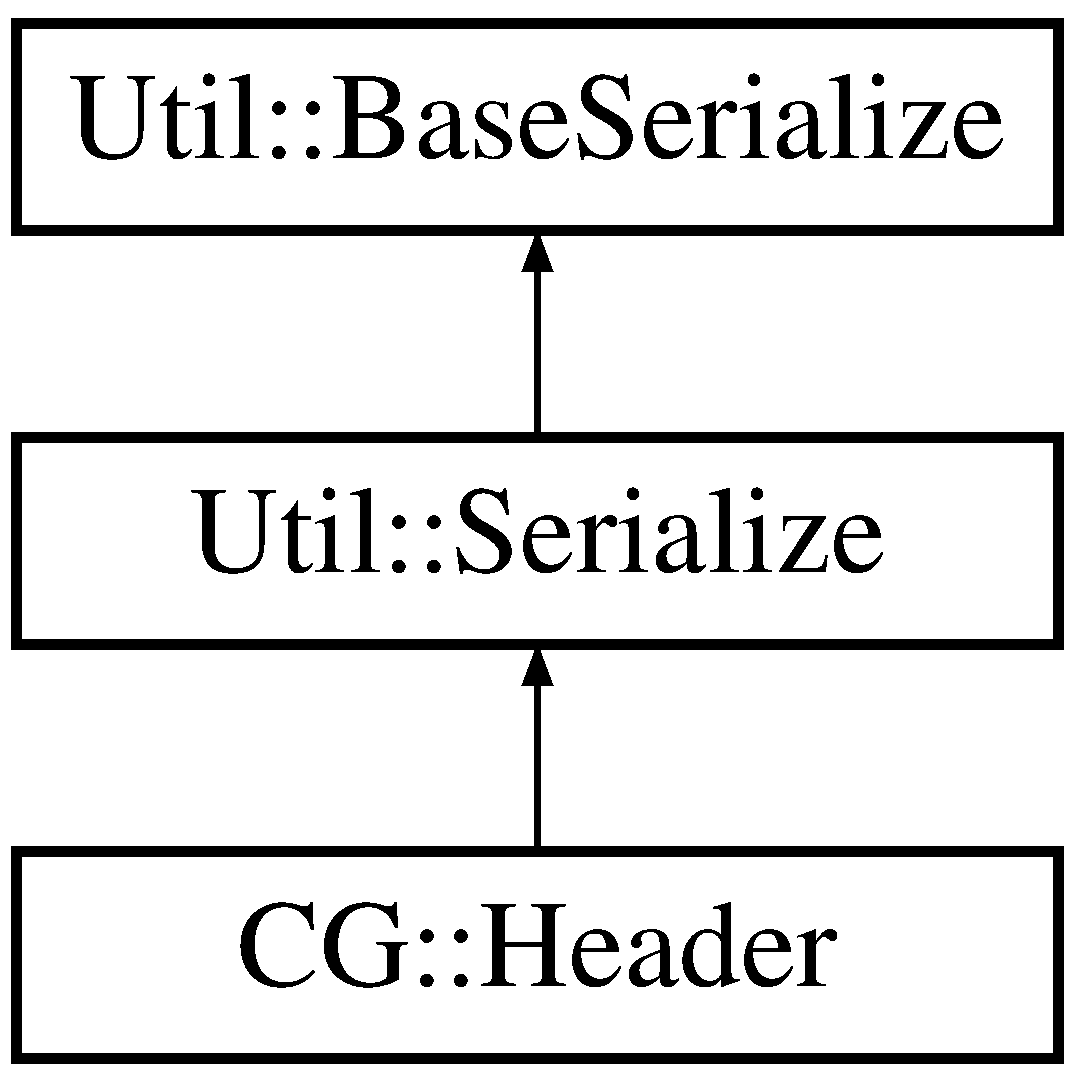
\includegraphics[height=3.000000cm]{class_c_g_1_1_header}
\end{center}
\end{figure}
\subsection*{Public Attributes}
\begin{DoxyCompactItemize}
\item 
\mbox{\Hypertarget{class_c_g_1_1_header_ad3df9a72b81681aec34ac69b0819e1ab}\label{class_c_g_1_1_header_ad3df9a72b81681aec34ac69b0819e1ab}} 
np\+Type\+\_\+t {\bfseries np\+Type}
\item 
\mbox{\Hypertarget{class_c_g_1_1_header_a76633474a7a00ba8b262a8a5210c41a7}\label{class_c_g_1_1_header_a76633474a7a00ba8b262a8a5210c41a7}} 
np\+Size\+\_\+t {\bfseries np\+Size}
\end{DoxyCompactItemize}
\subsection*{Additional Inherited Members}


The documentation for this class was generated from the following file\+:\begin{DoxyCompactItemize}
\item 
network/module/packet/Network\+Packet.\+h\end{DoxyCompactItemize}

\hypertarget{class_util_1_1_int_packet}{}\section{Util\+:\+:Int\+Packet Class Reference}
\label{class_util_1_1_int_packet}\index{Util\+::\+Int\+Packet@{Util\+::\+Int\+Packet}}
Inheritance diagram for Util\+:\+:Int\+Packet\+:\begin{figure}[H]
\begin{center}
\leavevmode
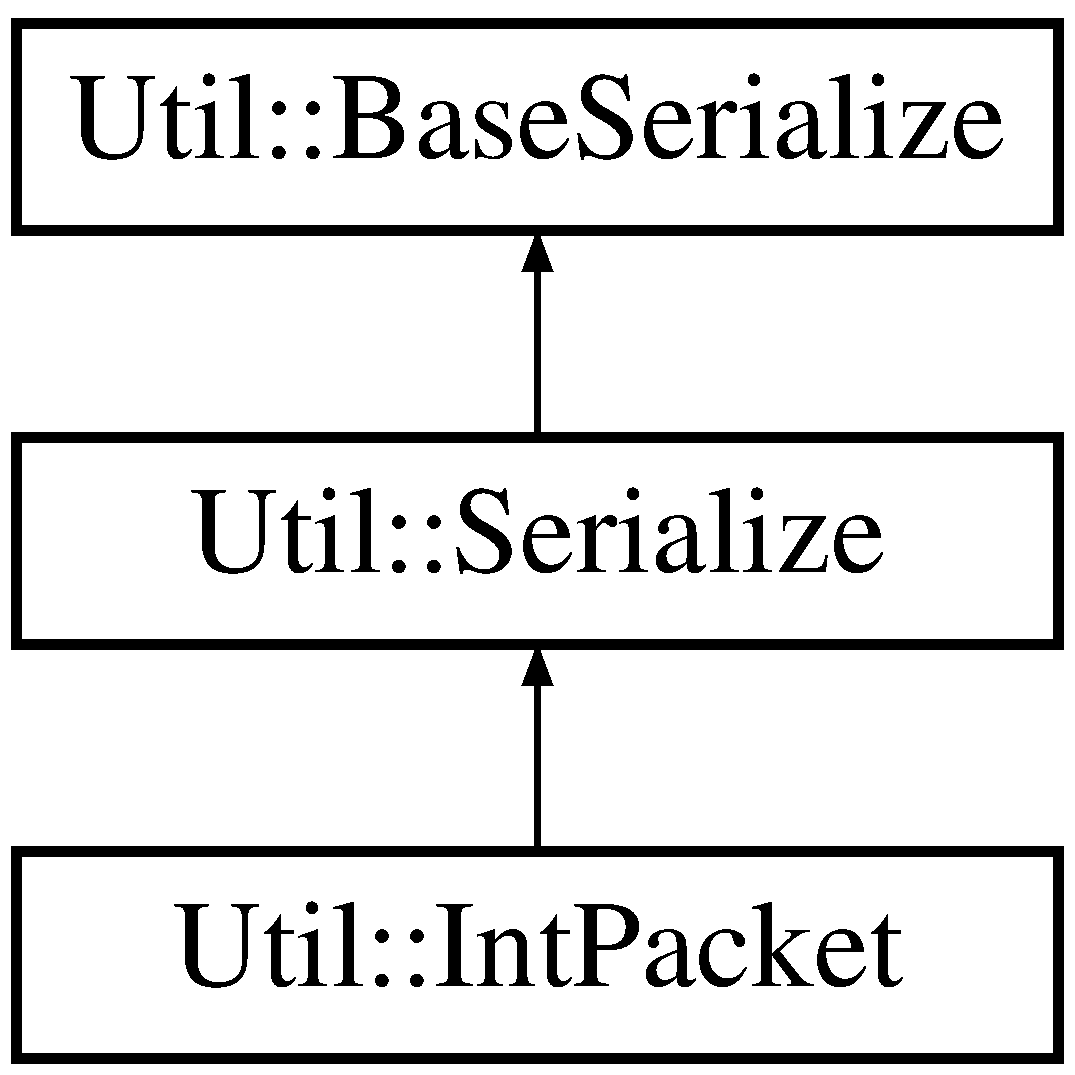
\includegraphics[height=3.000000cm]{class_util_1_1_int_packet}
\end{center}
\end{figure}
\subsection*{Public Attributes}
\begin{DoxyCompactItemize}
\item 
\mbox{\Hypertarget{class_util_1_1_int_packet_af245b2ee6510410bca9880681fd6754e}\label{class_util_1_1_int_packet_af245b2ee6510410bca9880681fd6754e}} 
int32\+\_\+t {\bfseries value}
\end{DoxyCompactItemize}
\subsection*{Additional Inherited Members}


The documentation for this class was generated from the following file\+:\begin{DoxyCompactItemize}
\item 
util/serialize/Serialize.\+h\end{DoxyCompactItemize}

\hypertarget{class_util_1_1_list}{}\section{Util\+:\+:List$<$ T $>$ Class Template Reference}
\label{class_util_1_1_list}\index{Util\+::\+List$<$ T $>$@{Util\+::\+List$<$ T $>$}}
Inheritance diagram for Util\+:\+:List$<$ T $>$\+:\begin{figure}[H]
\begin{center}
\leavevmode
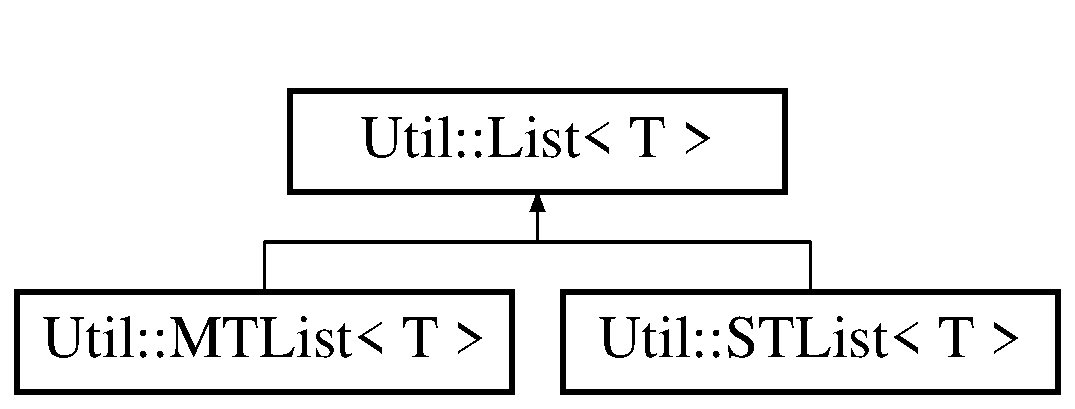
\includegraphics[height=2.000000cm]{class_util_1_1_list}
\end{center}
\end{figure}
\subsection*{Public Member Functions}
\begin{DoxyCompactItemize}
\item 
\mbox{\Hypertarget{class_util_1_1_list_a2a86bc77ae5dd6ace5770664acad9d77}\label{class_util_1_1_list_a2a86bc77ae5dd6ace5770664acad9d77}} 
virtual T {\bfseries at} (int index)=0
\item 
\mbox{\Hypertarget{class_util_1_1_list_a762c1a9516ac1da67fbc49ffa134ea89}\label{class_util_1_1_list_a762c1a9516ac1da67fbc49ffa134ea89}} 
virtual bool {\bfseries remove} (T t)=0
\item 
\mbox{\Hypertarget{class_util_1_1_list_a7619f2ffda6b42c87d19cfce4dc777a0}\label{class_util_1_1_list_a7619f2ffda6b42c87d19cfce4dc777a0}} 
virtual bool {\bfseries remove} (int index)=0
\item 
\mbox{\Hypertarget{class_util_1_1_list_a1b01b9b733e9f1fff71e117f7dd247b7}\label{class_util_1_1_list_a1b01b9b733e9f1fff71e117f7dd247b7}} 
virtual void {\bfseries push\+\_\+back} (T t)=0
\item 
\mbox{\Hypertarget{class_util_1_1_list_a2d41f217eb8af34c90f6f616554a4345}\label{class_util_1_1_list_a2d41f217eb8af34c90f6f616554a4345}} 
virtual int {\bfseries size} ()=0
\end{DoxyCompactItemize}


The documentation for this class was generated from the following file\+:\begin{DoxyCompactItemize}
\item 
util/list/List.\+h\end{DoxyCompactItemize}

\hypertarget{class_util_1_1_lock}{}\section{Util\+:\+:Lock Class Reference}
\label{class_util_1_1_lock}\index{Util\+::\+Lock@{Util\+::\+Lock}}
Inheritance diagram for Util\+:\+:Lock\+:\begin{figure}[H]
\begin{center}
\leavevmode
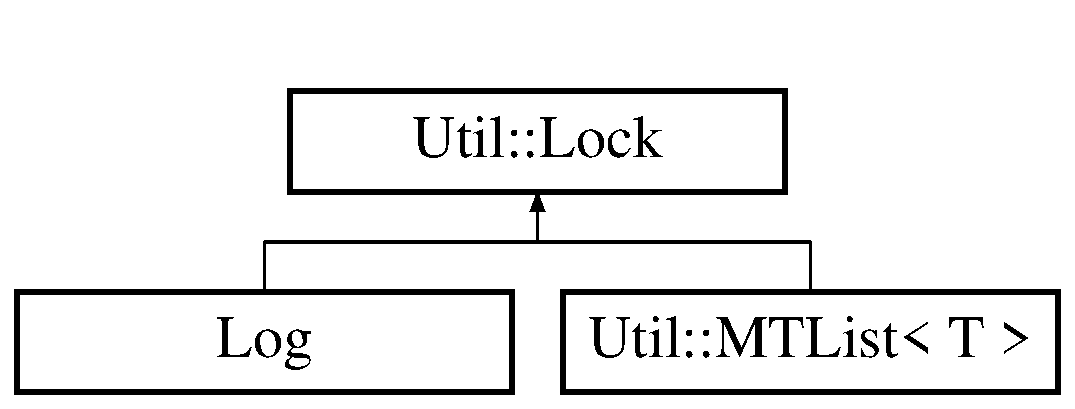
\includegraphics[height=2.000000cm]{class_util_1_1_lock}
\end{center}
\end{figure}
\subsection*{Protected Member Functions}
\begin{DoxyCompactItemize}
\item 
\mbox{\Hypertarget{class_util_1_1_lock_a2d72c766879141194ba56eded4c5f393}\label{class_util_1_1_lock_a2d72c766879141194ba56eded4c5f393}} 
void {\bfseries lock} ()
\item 
\mbox{\Hypertarget{class_util_1_1_lock_a937cc82b6f7acf16ecbdca9c5bc751f4}\label{class_util_1_1_lock_a937cc82b6f7acf16ecbdca9c5bc751f4}} 
void {\bfseries un\+Lock} ()
\end{DoxyCompactItemize}
\subsection*{Protected Attributes}
\begin{DoxyCompactItemize}
\item 
\mbox{\Hypertarget{class_util_1_1_lock_a6ab60541566026a346de5b4bd59f3e66}\label{class_util_1_1_lock_a6ab60541566026a346de5b4bd59f3e66}} 
std\+::mutex {\bfseries mutex}
\end{DoxyCompactItemize}


The documentation for this class was generated from the following file\+:\begin{DoxyCompactItemize}
\item 
util/lock/Lock.\+h\end{DoxyCompactItemize}

\hypertarget{class_log}{}\section{Log Class Reference}
\label{class_log}\index{Log@{Log}}
Inheritance diagram for Log\+:\begin{figure}[H]
\begin{center}
\leavevmode
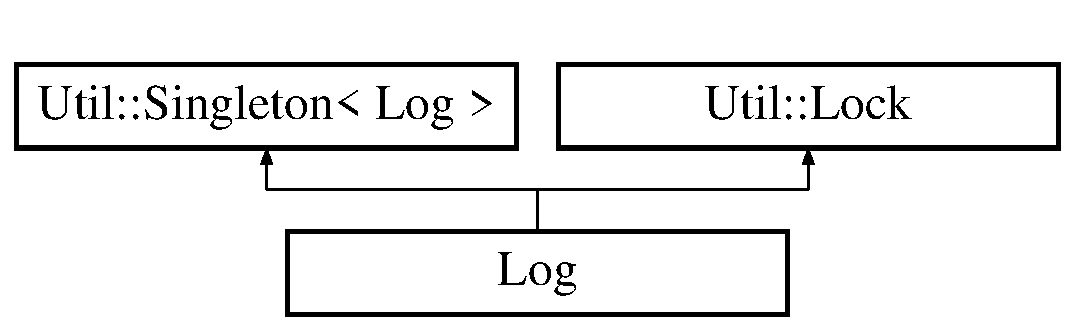
\includegraphics[height=2.000000cm]{class_log}
\end{center}
\end{figure}
\subsection*{Public Member Functions}
\begin{DoxyCompactItemize}
\item 
\mbox{\Hypertarget{class_log_a3e67ef6fb8b7e022f7c8273594b19081}\label{class_log_a3e67ef6fb8b7e022f7c8273594b19081}} 
bool {\bfseries initialize} (const char $\ast$logpath)
\item 
\mbox{\Hypertarget{class_log_a1206662f5fa82b744e79f554ca614e73}\label{class_log_a1206662f5fa82b744e79f554ca614e73}} 
bool {\bfseries create\+File} ()
\item 
\mbox{\Hypertarget{class_log_ab68da125c42590ef825900948e8239df}\label{class_log_ab68da125c42590ef825900948e8239df}} 
void {\bfseries print} (logtype type, const char $\ast$fmt,...)
\end{DoxyCompactItemize}
\subsection*{Additional Inherited Members}


The documentation for this class was generated from the following files\+:\begin{DoxyCompactItemize}
\item 
log/Log.\+h\item 
log/Log.\+cpp\end{DoxyCompactItemize}

\hypertarget{class_c_g_1_1_message_packet}{}\section{CG\+:\+:Message\+Packet Class Reference}
\label{class_c_g_1_1_message_packet}\index{C\+G\+::\+Message\+Packet@{C\+G\+::\+Message\+Packet}}
Inheritance diagram for CG\+:\+:Message\+Packet\+:\begin{figure}[H]
\begin{center}
\leavevmode
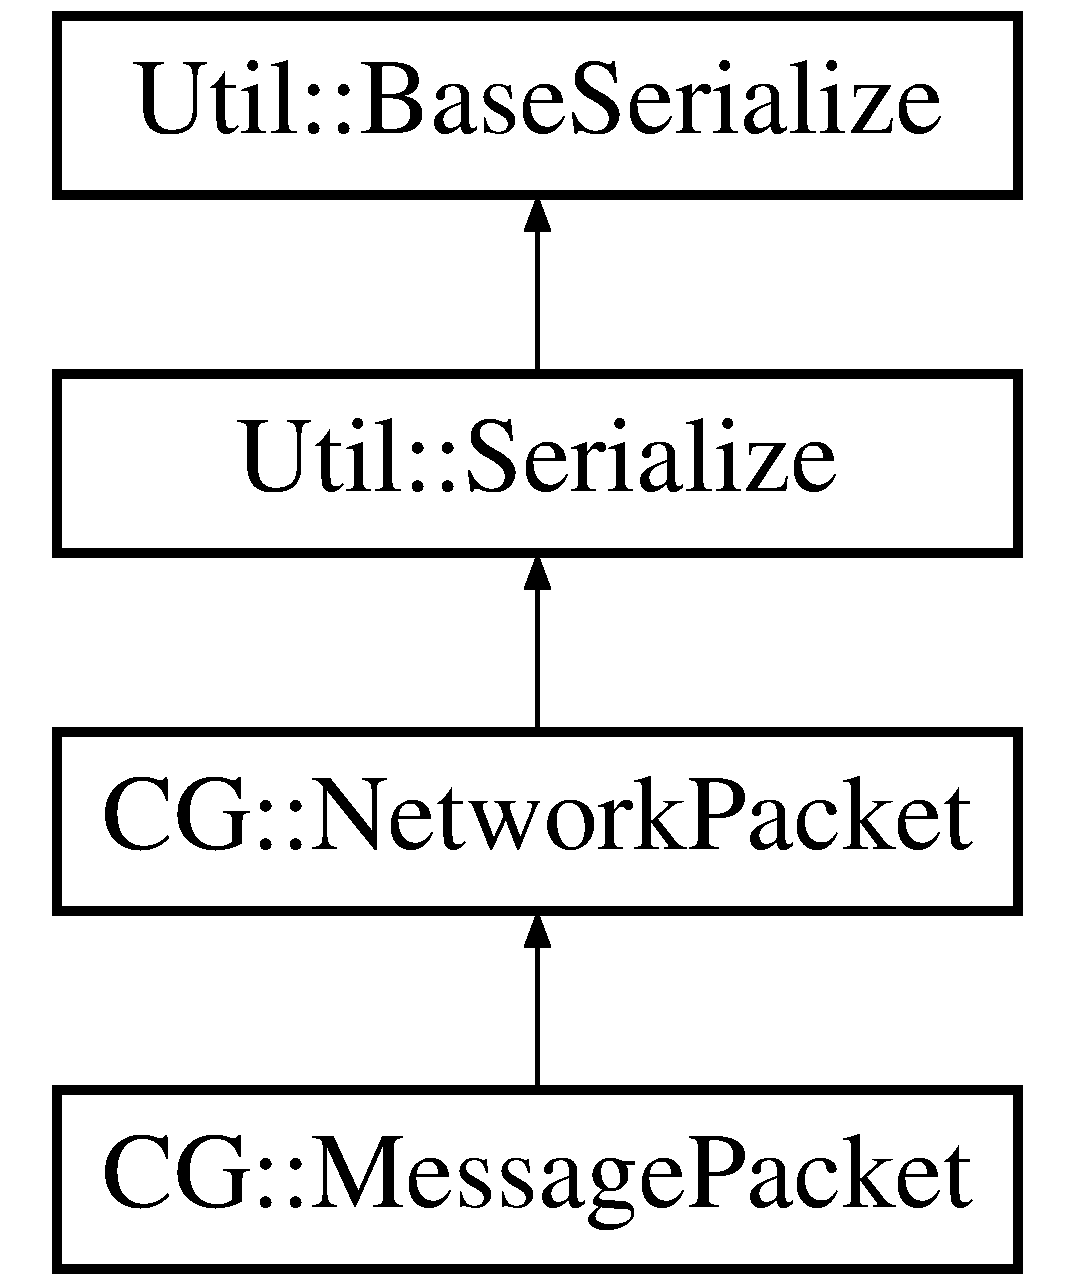
\includegraphics[height=4.000000cm]{class_c_g_1_1_message_packet}
\end{center}
\end{figure}
\subsection*{Public Attributes}
\begin{DoxyCompactItemize}
\item 
\mbox{\Hypertarget{class_c_g_1_1_message_packet_a75937c14ccb33df96a58444c747e6f24}\label{class_c_g_1_1_message_packet_a75937c14ccb33df96a58444c747e6f24}} 
std\+::string {\bfseries str}
\end{DoxyCompactItemize}
\subsection*{Additional Inherited Members}


The documentation for this class was generated from the following file\+:\begin{DoxyCompactItemize}
\item 
network/module/packet/Network\+Packet.\+h\end{DoxyCompactItemize}

\hypertarget{class_util_1_1_m_t_list}{}\section{Util\+:\+:M\+T\+List$<$ T $>$ Class Template Reference}
\label{class_util_1_1_m_t_list}\index{Util\+::\+M\+T\+List$<$ T $>$@{Util\+::\+M\+T\+List$<$ T $>$}}
Inheritance diagram for Util\+:\+:M\+T\+List$<$ T $>$\+:\begin{figure}[H]
\begin{center}
\leavevmode
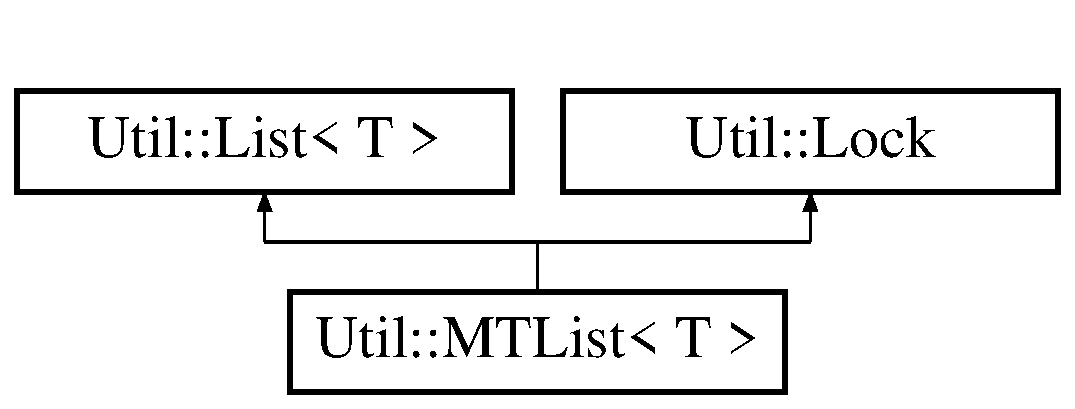
\includegraphics[height=2.000000cm]{class_util_1_1_m_t_list}
\end{center}
\end{figure}
\subsection*{Public Member Functions}
\begin{DoxyCompactItemize}
\item 
\mbox{\Hypertarget{class_util_1_1_m_t_list_a7e1566aab4a9ad96040f3b3f01497f1f}\label{class_util_1_1_m_t_list_a7e1566aab4a9ad96040f3b3f01497f1f}} 
T {\bfseries at} (int index)
\item 
\mbox{\Hypertarget{class_util_1_1_m_t_list_ab11f67bde61e13b40e335cec141a16ce}\label{class_util_1_1_m_t_list_ab11f67bde61e13b40e335cec141a16ce}} 
bool {\bfseries remove} (T t)
\item 
\mbox{\Hypertarget{class_util_1_1_m_t_list_a5d23f7ee870b82e5be693816f0db59c6}\label{class_util_1_1_m_t_list_a5d23f7ee870b82e5be693816f0db59c6}} 
bool {\bfseries remove} (int index)
\item 
\mbox{\Hypertarget{class_util_1_1_m_t_list_a383ad763ad7921b72d3325e277f0c6ac}\label{class_util_1_1_m_t_list_a383ad763ad7921b72d3325e277f0c6ac}} 
void {\bfseries push\+\_\+back} (T t)
\item 
\mbox{\Hypertarget{class_util_1_1_m_t_list_a98e0fb5c481e40f8f251e94b0705f880}\label{class_util_1_1_m_t_list_a98e0fb5c481e40f8f251e94b0705f880}} 
int {\bfseries size} ()
\end{DoxyCompactItemize}
\subsection*{Protected Attributes}
\begin{DoxyCompactItemize}
\item 
\mbox{\Hypertarget{class_util_1_1_m_t_list_abfaba74b7870494e8b4d8670b6ed7712}\label{class_util_1_1_m_t_list_abfaba74b7870494e8b4d8670b6ed7712}} 
std\+::vector$<$ T $>$ {\bfseries object\+List}
\end{DoxyCompactItemize}
\subsection*{Additional Inherited Members}


The documentation for this class was generated from the following file\+:\begin{DoxyCompactItemize}
\item 
util/list/M\+T\+List.\+h\end{DoxyCompactItemize}

\hypertarget{class_util_1_1_n_b_queue}{}\section{Util\+:\+:N\+B\+Queue$<$ T $>$ Class Template Reference}
\label{class_util_1_1_n_b_queue}\index{Util\+::\+N\+B\+Queue$<$ T $>$@{Util\+::\+N\+B\+Queue$<$ T $>$}}
Inheritance diagram for Util\+:\+:N\+B\+Queue$<$ T $>$\+:\begin{figure}[H]
\begin{center}
\leavevmode
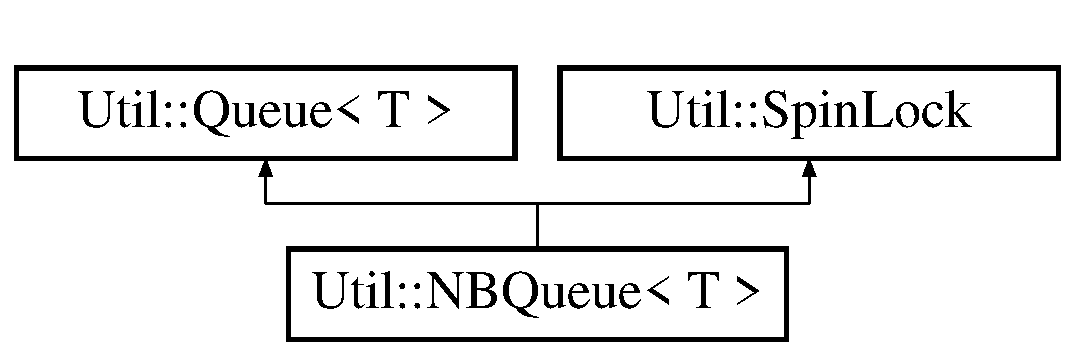
\includegraphics[height=2.000000cm]{class_util_1_1_n_b_queue}
\end{center}
\end{figure}
\subsection*{Public Member Functions}
\begin{DoxyCompactItemize}
\item 
\mbox{\Hypertarget{class_util_1_1_n_b_queue_a6e5c795a78408bdc90b22b063d19bf05}\label{class_util_1_1_n_b_queue_a6e5c795a78408bdc90b22b063d19bf05}} 
T {\bfseries pop} ()
\item 
\mbox{\Hypertarget{class_util_1_1_n_b_queue_a80e0acaf08e1aff29624310c26080d08}\label{class_util_1_1_n_b_queue_a80e0acaf08e1aff29624310c26080d08}} 
void {\bfseries push} (T t)
\item 
\mbox{\Hypertarget{class_util_1_1_n_b_queue_a9c6d5bc11f1ce6f946e77ca680c02e28}\label{class_util_1_1_n_b_queue_a9c6d5bc11f1ce6f946e77ca680c02e28}} 
int {\bfseries size} ()
\end{DoxyCompactItemize}
\subsection*{Public Attributes}
\begin{DoxyCompactItemize}
\item 
\mbox{\Hypertarget{class_util_1_1_n_b_queue_adb5b1aa5336d83df053fd4912b16e739}\label{class_util_1_1_n_b_queue_adb5b1aa5336d83df053fd4912b16e739}} 
std\+::queue$<$ T $>$ {\bfseries object\+Queue}
\end{DoxyCompactItemize}
\subsection*{Additional Inherited Members}


The documentation for this class was generated from the following file\+:\begin{DoxyCompactItemize}
\item 
util/queue/N\+B\+Queue.\+h\end{DoxyCompactItemize}

\hypertarget{class_c_g_1_1_network}{}\section{CG\+:\+:Network Class Reference}
\label{class_c_g_1_1_network}\index{C\+G\+::\+Network@{C\+G\+::\+Network}}
Inheritance diagram for CG\+:\+:Network\+:\begin{figure}[H]
\begin{center}
\leavevmode
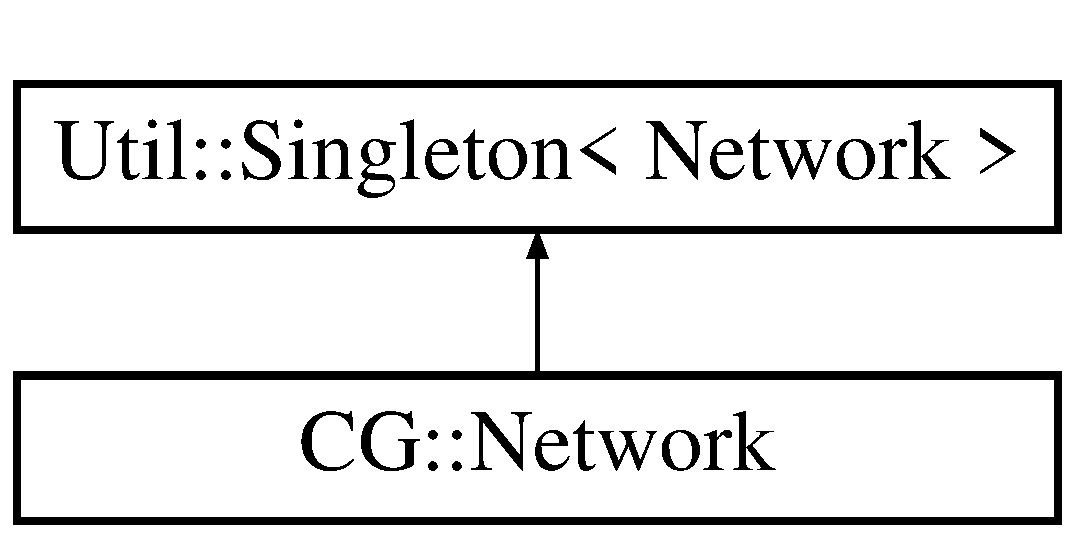
\includegraphics[height=2.000000cm]{class_c_g_1_1_network}
\end{center}
\end{figure}
\subsection*{Public Member Functions}
\begin{DoxyCompactItemize}
\item 
\mbox{\Hypertarget{class_c_g_1_1_network_ad78402e19997627dfdc66acc8d692454}\label{class_c_g_1_1_network_ad78402e19997627dfdc66acc8d692454}} 
long {\bfseries get\+Network\+Current\+Time} ()
\item 
\mbox{\Hypertarget{class_c_g_1_1_network_a8d3dc68aa1225515c64452fb6959ed4f}\label{class_c_g_1_1_network_a8d3dc68aa1225515c64452fb6959ed4f}} 
bool {\bfseries init} ()
\item 
\mbox{\Hypertarget{class_c_g_1_1_network_a2ee44c8a4cc822642315e22e8c6752e3}\label{class_c_g_1_1_network_a2ee44c8a4cc822642315e22e8c6752e3}} 
bool {\bfseries add\+Connector} (\mbox{\hyperlink{class_c_g_1_1_base_connector}{Base\+Connector}} $\ast$connect)
\item 
\mbox{\Hypertarget{class_c_g_1_1_network_a9bfaa8c8baf2cabe501b03e425b9b95a}\label{class_c_g_1_1_network_a9bfaa8c8baf2cabe501b03e425b9b95a}} 
bool {\bfseries add\+Server} (\mbox{\hyperlink{class_c_g_1_1_base_server}{Base\+Server}} $\ast$server)
\item 
\mbox{\Hypertarget{class_c_g_1_1_network_af1718e351ac7f026414854c082cac37c}\label{class_c_g_1_1_network_af1718e351ac7f026414854c082cac37c}} 
bool {\bfseries add\+Client} (\mbox{\hyperlink{class_c_g_1_1_base_client}{Base\+Client}} $\ast$client)
\item 
\mbox{\Hypertarget{class_c_g_1_1_network_a866f5d6275992de290a5e9754c526e6a}\label{class_c_g_1_1_network_a866f5d6275992de290a5e9754c526e6a}} 
int {\bfseries Create\+T\+C\+P\+Server\+Socket} (const char $\ast$ip, unsigned short port)
\item 
\mbox{\Hypertarget{class_c_g_1_1_network_a7caa058a41315430ba5dc051739bf3df}\label{class_c_g_1_1_network_a7caa058a41315430ba5dc051739bf3df}} 
int {\bfseries Create\+T\+C\+P\+Client\+Socket} (const char $\ast$ip, unsigned short port)
\item 
\mbox{\Hypertarget{class_c_g_1_1_network_ab9d768fbb1ffe711c3bf7e1fa38c12ee}\label{class_c_g_1_1_network_ab9d768fbb1ffe711c3bf7e1fa38c12ee}} 
bool {\bfseries add\+Timer} (\mbox{\hyperlink{class_c_g_1_1_timer}{Timer}} $\ast$timer)
\item 
\mbox{\Hypertarget{class_c_g_1_1_network_a5db4a0eed7fa669c64ab1fdacb75a9de}\label{class_c_g_1_1_network_a5db4a0eed7fa669c64ab1fdacb75a9de}} 
void {\bfseries send\+Data} (int fd, const char $\ast$data, int data\+Size)
\item 
\mbox{\Hypertarget{class_c_g_1_1_network_aac7198d5ba6e0add2257e0da3943f756}\label{class_c_g_1_1_network_aac7198d5ba6e0add2257e0da3943f756}} 
void {\bfseries send\+Data} (\mbox{\hyperlink{class_c_g_1_1_base_connector}{Base\+Connector}} $\ast$connector, const char $\ast$data, int data\+Size)
\item 
\mbox{\Hypertarget{class_c_g_1_1_network_aeafac10483418b385c2e183c8516610e}\label{class_c_g_1_1_network_aeafac10483418b385c2e183c8516610e}} 
void {\bfseries send\+Data} (\mbox{\hyperlink{class_c_g_1_1_connector_info}{Connector\+Info}} $\ast$connector\+Info, const char $\ast$data, int data\+Size)
\item 
\mbox{\Hypertarget{class_c_g_1_1_network_ac13d409479954945a69ae573ac89d639}\label{class_c_g_1_1_network_ac13d409479954945a69ae573ac89d639}} 
bool {\bfseries process\+Receive\+Data} (\mbox{\hyperlink{class_c_g_1_1_connector_info}{Connector\+Info}} $\ast$connector\+Info)
\item 
\mbox{\Hypertarget{class_c_g_1_1_network_a40e2c5ec8e896caa93fd5ca30fe8d837}\label{class_c_g_1_1_network_a40e2c5ec8e896caa93fd5ca30fe8d837}} 
\mbox{\hyperlink{class_c_g_1_1_worker_thread}{Worker\+Thread}} $\ast$ {\bfseries get\+Worker\+Thread\+Using\+Hash} (int hash\+Key)
\item 
\mbox{\Hypertarget{class_c_g_1_1_network_a5366aa30553b7e4f92fc936301448eec}\label{class_c_g_1_1_network_a5366aa30553b7e4f92fc936301448eec}} 
void {\bfseries disconnect\+With\+Connector\+Info} (\mbox{\hyperlink{class_c_g_1_1_worker_thread}{Worker\+Thread}} $\ast$worker\+Thread, \mbox{\hyperlink{class_c_g_1_1_connector_info}{Connector\+Info}} $\ast$connector\+Info)
\item 
\mbox{\Hypertarget{class_c_g_1_1_network_add107d404897c8f29669fd1210ebec17}\label{class_c_g_1_1_network_add107d404897c8f29669fd1210ebec17}} 
void {\bfseries start} ()
\item 
\mbox{\Hypertarget{class_c_g_1_1_network_a8ef3e5635ff4eb5a1e75d02e82b6bc3f}\label{class_c_g_1_1_network_a8ef3e5635ff4eb5a1e75d02e82b6bc3f}} 
void {\bfseries windows\+Connector\+Info\+Thread} (\mbox{\hyperlink{class_c_g_1_1_connector_info}{Connector\+Info}} $\ast$connector\+Info)
\item 
\mbox{\Hypertarget{class_c_g_1_1_network_a54d8280ebfdb0b0956a81b21f3ea30a4}\label{class_c_g_1_1_network_a54d8280ebfdb0b0956a81b21f3ea30a4}} 
void {\bfseries windows\+Server\+Thread} (\mbox{\hyperlink{class_c_g_1_1_base_server}{Base\+Server}} $\ast$server)
\end{DoxyCompactItemize}
\subsection*{Static Public Member Functions}
\begin{DoxyCompactItemize}
\item 
\mbox{\Hypertarget{class_c_g_1_1_network_aad38df455a3c12db45492a1a1487ca87}\label{class_c_g_1_1_network_aad38df455a3c12db45492a1a1487ca87}} 
static void $\ast$ {\bfseries start\+Unix\+Running\+Thread} (void $\ast$a)
\end{DoxyCompactItemize}
\subsection*{Public Attributes}
\begin{DoxyCompactItemize}
\item 
\mbox{\Hypertarget{class_c_g_1_1_network_a6130f231ce02cf35083675b1f08d941d}\label{class_c_g_1_1_network_a6130f231ce02cf35083675b1f08d941d}} 
int {\bfseries worker\+Thread\+Count}
\item 
\mbox{\Hypertarget{class_c_g_1_1_network_a7bbcc20e73d8ffd3cc5c1e9b5ca45653}\label{class_c_g_1_1_network_a7bbcc20e73d8ffd3cc5c1e9b5ca45653}} 
\mbox{\hyperlink{class_c_g_1_1_worker_thread}{Worker\+Thread}} $\ast$$\ast$ {\bfseries worker\+Thread\+Array}
\item 
\mbox{\Hypertarget{class_c_g_1_1_network_a12e773c9b3a524ba449baaae26465578}\label{class_c_g_1_1_network_a12e773c9b3a524ba449baaae26465578}} 
\mbox{\hyperlink{class_util_1_1_list}{Util\+::\+List}}$<$ \mbox{\hyperlink{class_c_g_1_1_base_server}{Base\+Server}} $\ast$ $>$ $\ast$ {\bfseries server\+List}
\item 
\mbox{\Hypertarget{class_c_g_1_1_network_accc7187702968499740a9de2dca33d32}\label{class_c_g_1_1_network_accc7187702968499740a9de2dca33d32}} 
\mbox{\hyperlink{class_util_1_1_list}{Util\+::\+List}}$<$ \mbox{\hyperlink{class_c_g_1_1_base_client}{Base\+Client}} $\ast$ $>$ $\ast$ {\bfseries client\+List}
\item 
\mbox{\Hypertarget{class_c_g_1_1_network_a00a784ea618276fe54ab09dd4f57a301}\label{class_c_g_1_1_network_a00a784ea618276fe54ab09dd4f57a301}} 
\mbox{\hyperlink{class_util_1_1_queue}{Util\+::\+Queue}}$<$ \mbox{\hyperlink{class_c_g_1_1_timer}{Timer}} $\ast$ $>$ $\ast$ {\bfseries timer\+Queue}
\item 
\mbox{\Hypertarget{class_c_g_1_1_network_a0c66272858b3eb446fe80a0810dd7b8c}\label{class_c_g_1_1_network_a0c66272858b3eb446fe80a0810dd7b8c}} 
int {\bfseries event\+Fd}
\item 
\mbox{\Hypertarget{class_c_g_1_1_network_aaa0677f4142005c8180d9d84d550e4c9}\label{class_c_g_1_1_network_aaa0677f4142005c8180d9d84d550e4c9}} 
int {\bfseries clnt\+Fd}
\item 
\mbox{\Hypertarget{class_c_g_1_1_network_a12d20e697fc95c76b907073666ea622b}\label{class_c_g_1_1_network_a12d20e697fc95c76b907073666ea622b}} 
struct sockaddr\+\_\+in {\bfseries clntaddr}
\item 
\mbox{\Hypertarget{class_c_g_1_1_network_acb771586a3f23f2be7690042d9b15a65}\label{class_c_g_1_1_network_acb771586a3f23f2be7690042d9b15a65}} 
int {\bfseries clntaddr\+Len}
\item 
\mbox{\Hypertarget{class_c_g_1_1_network_a837eb0caccdff8c61fa0328ae1a6d8e4}\label{class_c_g_1_1_network_a837eb0caccdff8c61fa0328ae1a6d8e4}} 
long {\bfseries current\+Time}
\item 
\mbox{\Hypertarget{class_c_g_1_1_network_acd01adbd56173cb7166962ef3048b26e}\label{class_c_g_1_1_network_acd01adbd56173cb7166962ef3048b26e}} 
long {\bfseries last\+Loop\+Time}
\item 
\mbox{\Hypertarget{class_c_g_1_1_network_addf461a11555689ffd101b9432fa5f75}\label{class_c_g_1_1_network_addf461a11555689ffd101b9432fa5f75}} 
long {\bfseries loop\+Dt}
\item 
\mbox{\Hypertarget{class_c_g_1_1_network_a5493ef1349b446a6bf66ca5e1c71332a}\label{class_c_g_1_1_network_a5493ef1349b446a6bf66ca5e1c71332a}} 
std\+::thread {\bfseries network\+Thread}
\item 
\mbox{\Hypertarget{class_c_g_1_1_network_ab5b9827e5c8f6f92061d1ed24815a376}\label{class_c_g_1_1_network_ab5b9827e5c8f6f92061d1ed24815a376}} 
\mbox{\hyperlink{class_util_1_1_list}{Util\+::\+List}}$<$ std\+::thread $\ast$ $>$ $\ast$ {\bfseries server\+Thread\+List}
\item 
\mbox{\Hypertarget{class_c_g_1_1_network_adc43d39338d556987d0cf8c90851a7d4}\label{class_c_g_1_1_network_adc43d39338d556987d0cf8c90851a7d4}} 
\mbox{\hyperlink{class_util_1_1_list}{Util\+::\+List}}$<$ std\+::thread $\ast$ $>$ $\ast$ {\bfseries client\+Thread\+List}
\item 
\mbox{\Hypertarget{class_c_g_1_1_network_a3d2ccbb2cab8bcaf45bf270d67b087bd}\label{class_c_g_1_1_network_a3d2ccbb2cab8bcaf45bf270d67b087bd}} 
\mbox{\hyperlink{class_util_1_1_object_pool}{Util\+::\+Object\+Pool}}$<$ \mbox{\hyperlink{class_c_g_1_1_connector_info}{Connector\+Info}} $>$ $\ast$ {\bfseries connector\+Info\+Pool}
\end{DoxyCompactItemize}


The documentation for this class was generated from the following files\+:\begin{DoxyCompactItemize}
\item 
network/core/Network.\+h\item 
network/core/Network.\+cpp\end{DoxyCompactItemize}

\hypertarget{class_c_g_1_1_network_handler}{}\section{CG\+:\+:Network\+Handler Class Reference}
\label{class_c_g_1_1_network_handler}\index{C\+G\+::\+Network\+Handler@{C\+G\+::\+Network\+Handler}}
\subsection*{Public Member Functions}
\begin{DoxyCompactItemize}
\item 
\mbox{\Hypertarget{class_c_g_1_1_network_handler_afa93c724ce75d936ff506e020a98c297}\label{class_c_g_1_1_network_handler_afa93c724ce75d936ff506e020a98c297}} 
{\bfseries Network\+Handler} (std\+::function$<$ void(Host\+Id, char $\ast$, int)$>$ $\ast$\+\_\+on\+Receive)
\item 
\mbox{\Hypertarget{class_c_g_1_1_network_handler_a0b49efbd1bfdec05494df318880a6fe1}\label{class_c_g_1_1_network_handler_a0b49efbd1bfdec05494df318880a6fe1}} 
int {\bfseries process\+Data} (\mbox{\hyperlink{class_c_g_1_1_connector_info}{Connector\+Info}} $\ast$connector\+Info, char $\ast$data, int data\+Size)
\item 
\mbox{\Hypertarget{class_c_g_1_1_network_handler_ae423c0b4f16c5dd4f3dca1a1927fc910}\label{class_c_g_1_1_network_handler_ae423c0b4f16c5dd4f3dca1a1927fc910}} 
void {\bfseries send\+Message} (Host\+Id host\+Id, const char $\ast$data, int data\+Size)
\end{DoxyCompactItemize}
\subsection*{Public Attributes}
\begin{DoxyCompactItemize}
\item 
\mbox{\Hypertarget{class_c_g_1_1_network_handler_aac3677fc874325e5091be15ffee0cfcc}\label{class_c_g_1_1_network_handler_aac3677fc874325e5091be15ffee0cfcc}} 
std\+::function$<$ void(Host\+Id, char $\ast$, int)$>$ $\ast$ {\bfseries on\+Receive}
\end{DoxyCompactItemize}
\subsection*{Friends}
\begin{DoxyCompactItemize}
\item 
\mbox{\Hypertarget{class_c_g_1_1_network_handler_a88b59289ffd793fecd040d32e397b1e9}\label{class_c_g_1_1_network_handler_a88b59289ffd793fecd040d32e397b1e9}} 
class {\bfseries Network}
\end{DoxyCompactItemize}


The documentation for this class was generated from the following files\+:\begin{DoxyCompactItemize}
\item 
network/module/basic/Network\+Handler.\+h\item 
network/module/basic/Network\+Handler.\+cpp\end{DoxyCompactItemize}

\hypertarget{class_c_g_1_1_network_packet}{}\section{CG\+:\+:Network\+Packet Class Reference}
\label{class_c_g_1_1_network_packet}\index{C\+G\+::\+Network\+Packet@{C\+G\+::\+Network\+Packet}}
Inheritance diagram for CG\+:\+:Network\+Packet\+:\begin{figure}[H]
\begin{center}
\leavevmode
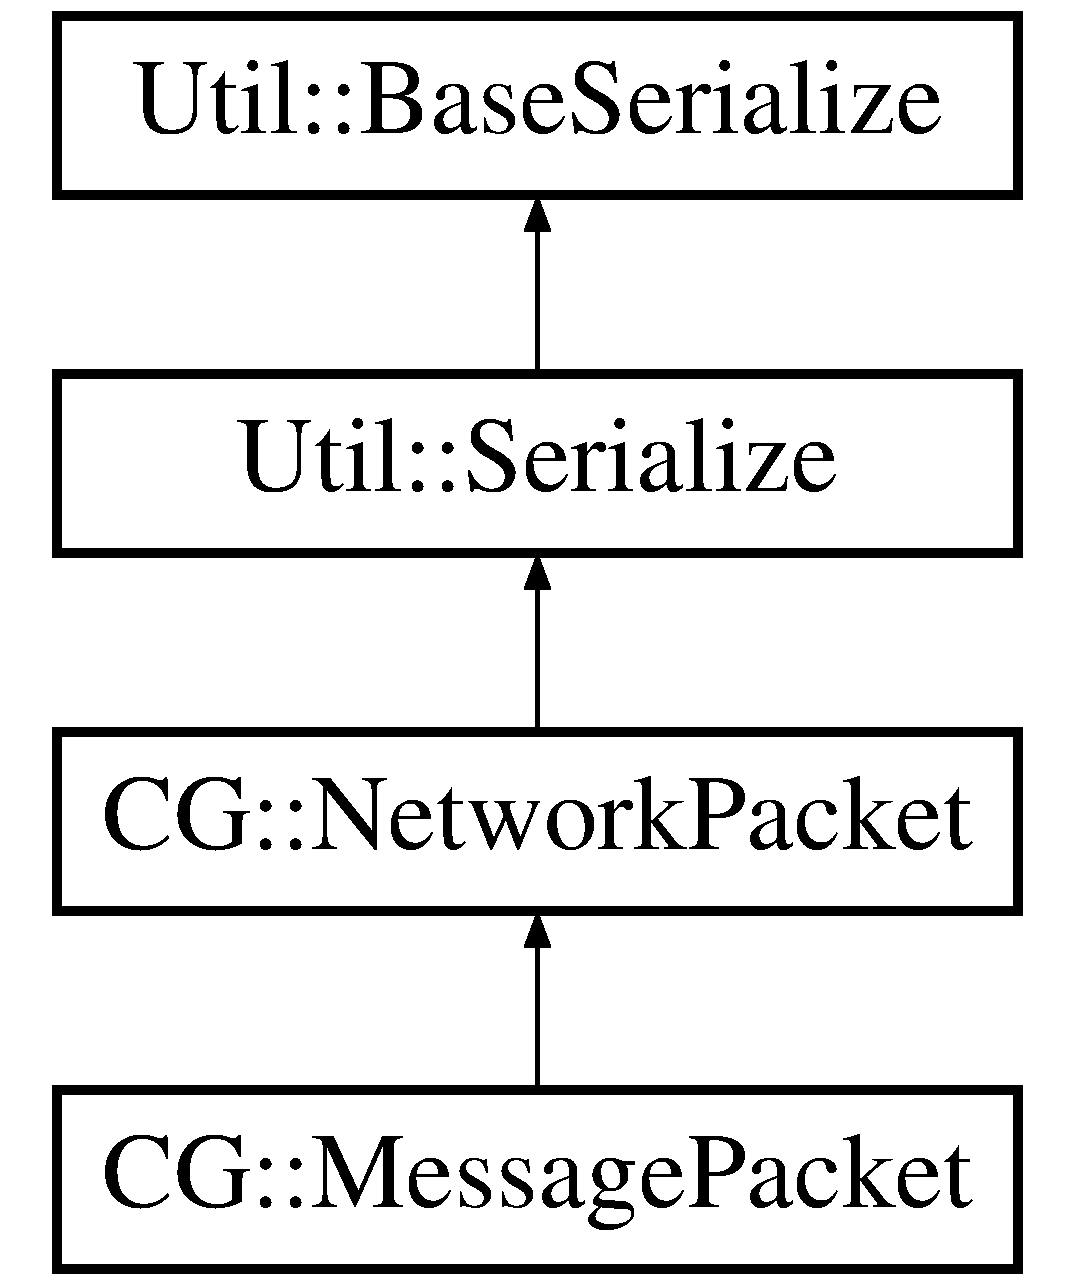
\includegraphics[height=4.000000cm]{class_c_g_1_1_network_packet}
\end{center}
\end{figure}
\subsection*{Public Member Functions}
\begin{DoxyCompactItemize}
\item 
\mbox{\Hypertarget{class_c_g_1_1_network_packet_a3c9a8ab2f895276adcc9f46ad0d90762}\label{class_c_g_1_1_network_packet_a3c9a8ab2f895276adcc9f46ad0d90762}} 
virtual \mbox{\hyperlink{class_c_g_1_1_network_packet}{Network\+Packet}} $\ast$ {\bfseries create} ()
\end{DoxyCompactItemize}
\subsection*{Public Attributes}
\begin{DoxyCompactItemize}
\item 
\mbox{\Hypertarget{class_c_g_1_1_network_packet_a79bfb6a2ab70562c2a9eaf3d13dbd224}\label{class_c_g_1_1_network_packet_a79bfb6a2ab70562c2a9eaf3d13dbd224}} 
\mbox{\hyperlink{class_c_g_1_1_header}{Header}} {\bfseries header}
\end{DoxyCompactItemize}


The documentation for this class was generated from the following file\+:\begin{DoxyCompactItemize}
\item 
network/module/packet/Network\+Packet.\+h\end{DoxyCompactItemize}

\hypertarget{class_c_g_1_1_n_p_serializer}{}\section{CG\+:\+:N\+P\+Serializer Class Reference}
\label{class_c_g_1_1_n_p_serializer}\index{C\+G\+::\+N\+P\+Serializer@{C\+G\+::\+N\+P\+Serializer}}
\subsection*{Public Member Functions}
\begin{DoxyCompactItemize}
\item 
\mbox{\Hypertarget{class_c_g_1_1_n_p_serializer_adc3e59852d676607157fba8e3416efca}\label{class_c_g_1_1_n_p_serializer_adc3e59852d676607157fba8e3416efca}} 
virtual int {\bfseries serialize} (char $\ast$buffer)=0
\item 
\mbox{\Hypertarget{class_c_g_1_1_n_p_serializer_ae939886560c4be1e3a2b1f3376299643}\label{class_c_g_1_1_n_p_serializer_ae939886560c4be1e3a2b1f3376299643}} 
virtual int {\bfseries deserialize} (const char $\ast$buffer)=0
\item 
\mbox{\Hypertarget{class_c_g_1_1_n_p_serializer_a7ee2183ac37127bd64bb6ab2ba1fa6e6}\label{class_c_g_1_1_n_p_serializer_a7ee2183ac37127bd64bb6ab2ba1fa6e6}} 
virtual int {\bfseries size} ()=0
\end{DoxyCompactItemize}
\subsection*{Public Attributes}
\begin{DoxyCompactItemize}
\item 
\mbox{\Hypertarget{class_c_g_1_1_n_p_serializer_a3edd1f4c2fed9b40e283b21f775cdf9a}\label{class_c_g_1_1_n_p_serializer_a3edd1f4c2fed9b40e283b21f775cdf9a}} 
std\+::list$<$ \mbox{\hyperlink{class_c_g_1_1_n_p_serializer}{N\+P\+Serializer}} $\ast$ $>$ {\bfseries nps\+List}
\end{DoxyCompactItemize}


The documentation for this class was generated from the following file\+:\begin{DoxyCompactItemize}
\item 
network/module/packet/Network\+Packet.\+h\end{DoxyCompactItemize}

\hypertarget{class_util_1_1_object_pool}{}\section{Util\+:\+:Object\+Pool$<$ T $>$ Class Template Reference}
\label{class_util_1_1_object_pool}\index{Util\+::\+Object\+Pool$<$ T $>$@{Util\+::\+Object\+Pool$<$ T $>$}}
\subsection*{Public Member Functions}
\begin{DoxyCompactItemize}
\item 
\mbox{\Hypertarget{class_util_1_1_object_pool_a05824b550fbbd97beee8ff7bdc7a1b6a}\label{class_util_1_1_object_pool_a05824b550fbbd97beee8ff7bdc7a1b6a}} 
{\bfseries Object\+Pool} (unsigned int capacity, bool is\+Using\+Multi\+Thread)
\item 
\mbox{\Hypertarget{class_util_1_1_object_pool_afe1d978de39c51f05aaa53aa3d466d27}\label{class_util_1_1_object_pool_afe1d978de39c51f05aaa53aa3d466d27}} 
T $\ast$ {\bfseries get\+Object} ()
\item 
\mbox{\Hypertarget{class_util_1_1_object_pool_af830036cb3f77b3264fa4468c713dbc5}\label{class_util_1_1_object_pool_af830036cb3f77b3264fa4468c713dbc5}} 
void {\bfseries return\+Object} (T $\ast$object)
\item 
\mbox{\Hypertarget{class_util_1_1_object_pool_a9be23d99fe9119b4a11d96aa78048121}\label{class_util_1_1_object_pool_a9be23d99fe9119b4a11d96aa78048121}} 
int {\bfseries size} ()
\end{DoxyCompactItemize}
\subsection*{Protected Attributes}
\begin{DoxyCompactItemize}
\item 
\mbox{\Hypertarget{class_util_1_1_object_pool_a9afa8e2e55e58041840e42d3b1c4b96f}\label{class_util_1_1_object_pool_a9afa8e2e55e58041840e42d3b1c4b96f}} 
\mbox{\hyperlink{class_util_1_1_queue}{Util\+::\+Queue}}$<$ T $\ast$ $>$ $\ast$ {\bfseries object\+List}
\item 
\mbox{\Hypertarget{class_util_1_1_object_pool_ac9c0d7430fa4c74ef62db2cb64d38b10}\label{class_util_1_1_object_pool_ac9c0d7430fa4c74ef62db2cb64d38b10}} 
unsigned int {\bfseries capacity}
\item 
\mbox{\Hypertarget{class_util_1_1_object_pool_aa5a993f164ed3f5ba4e7cda233fc64b8}\label{class_util_1_1_object_pool_aa5a993f164ed3f5ba4e7cda233fc64b8}} 
bool {\bfseries is\+Using\+Multi\+Thread}
\end{DoxyCompactItemize}


The documentation for this class was generated from the following file\+:\begin{DoxyCompactItemize}
\item 
util/object\+Pool/Object\+Pool.\+h\end{DoxyCompactItemize}

\hypertarget{class_c_g_1_1_packet_function}{}\section{CG\+:\+:Packet\+Function Class Reference}
\label{class_c_g_1_1_packet_function}\index{C\+G\+::\+Packet\+Function@{C\+G\+::\+Packet\+Function}}
\subsection*{Public Member Functions}
\begin{DoxyCompactItemize}
\item 
\mbox{\Hypertarget{class_c_g_1_1_packet_function_ad6e2c920b53d850ca57eb7d43a515790}\label{class_c_g_1_1_packet_function_ad6e2c920b53d850ca57eb7d43a515790}} 
{\bfseries Packet\+Function} (\mbox{\hyperlink{class_c_g_1_1_network_packet}{Network\+Packet}} $\ast$\+\_\+packet, std\+::function$<$ void(Host\+Id, \mbox{\hyperlink{class_c_g_1_1_network_packet}{Network\+Packet}} $\ast$)$>$ \+\_\+packet\+Function)
\end{DoxyCompactItemize}
\subsection*{Public Attributes}
\begin{DoxyCompactItemize}
\item 
\mbox{\Hypertarget{class_c_g_1_1_packet_function_a68ae3f738b28992508c174a7c9594f78}\label{class_c_g_1_1_packet_function_a68ae3f738b28992508c174a7c9594f78}} 
\mbox{\hyperlink{class_c_g_1_1_network_packet}{Network\+Packet}} $\ast$ {\bfseries packet}
\item 
\mbox{\Hypertarget{class_c_g_1_1_packet_function_ac96cd18a7b637cea1bd5f7db6b08570d}\label{class_c_g_1_1_packet_function_ac96cd18a7b637cea1bd5f7db6b08570d}} 
std\+::function$<$ void(Host\+Id, \mbox{\hyperlink{class_c_g_1_1_network_packet}{Network\+Packet}} $\ast$)$>$ {\bfseries packet\+Function}
\end{DoxyCompactItemize}


The documentation for this class was generated from the following file\+:\begin{DoxyCompactItemize}
\item 
network/module/packet/C\+G\+Network\+Handler.\+h\end{DoxyCompactItemize}

\hypertarget{class_c_g_1_1_peer}{}\section{CG\+:\+:Peer Class Reference}
\label{class_c_g_1_1_peer}\index{C\+G\+::\+Peer@{C\+G\+::\+Peer}}
Inheritance diagram for CG\+:\+:Peer\+:\begin{figure}[H]
\begin{center}
\leavevmode
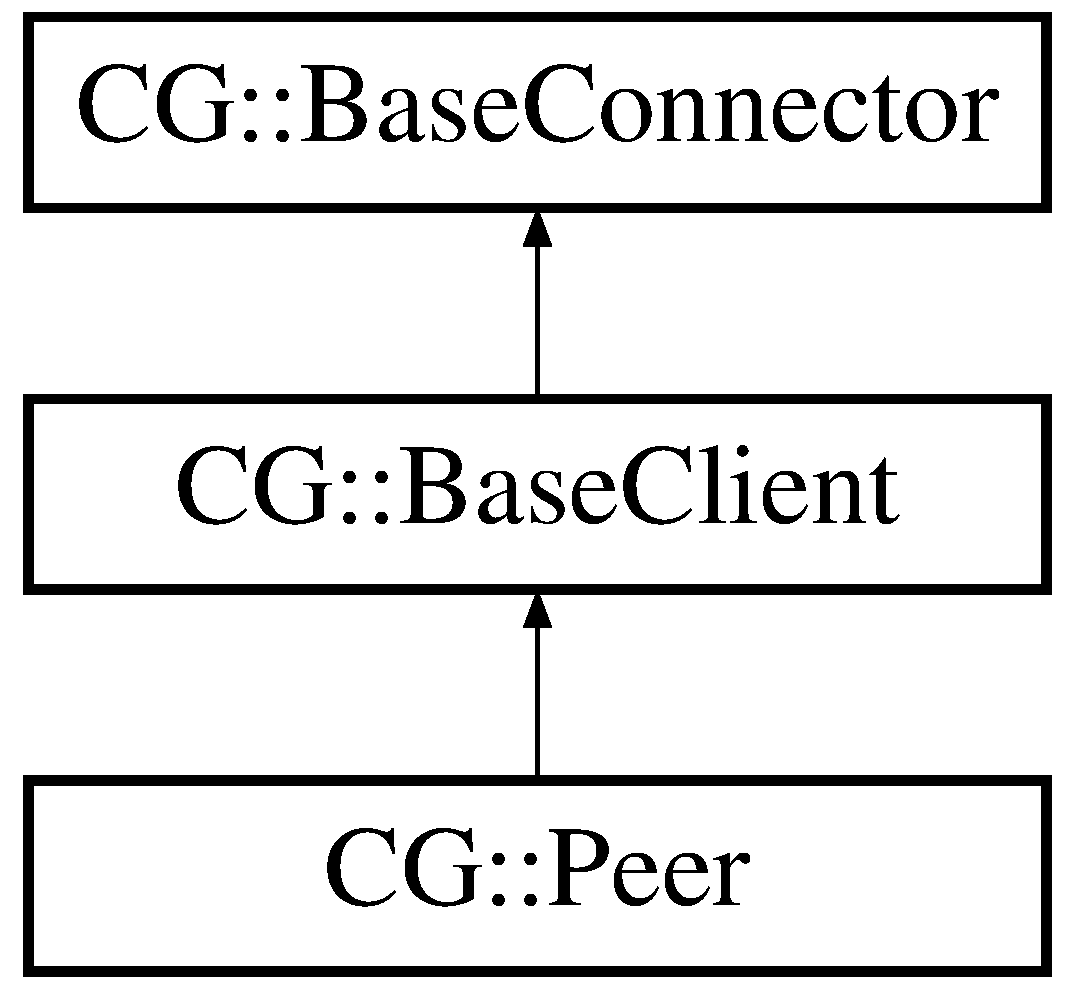
\includegraphics[height=3.000000cm]{class_c_g_1_1_peer}
\end{center}
\end{figure}
\subsection*{Public Member Functions}
\begin{DoxyCompactItemize}
\item 
\mbox{\Hypertarget{class_c_g_1_1_peer_ad7c328d003e82a45533302d09c273dc4}\label{class_c_g_1_1_peer_ad7c328d003e82a45533302d09c273dc4}} 
void {\bfseries send\+Message} (const char $\ast$data, int data\+Size)
\end{DoxyCompactItemize}
\subsection*{Additional Inherited Members}


The documentation for this class was generated from the following files\+:\begin{DoxyCompactItemize}
\item 
network/core/Peer.\+h\item 
network/core/Peer.\+cpp\end{DoxyCompactItemize}

\hypertarget{class_util_1_1_property}{}\section{Util\+:\+:Property$<$ T $>$ Class Template Reference}
\label{class_util_1_1_property}\index{Util\+::\+Property$<$ T $>$@{Util\+::\+Property$<$ T $>$}}
\subsection*{Public Member Functions}
\begin{DoxyCompactItemize}
\item 
\mbox{\Hypertarget{class_util_1_1_property_afea5192ef3d7fe210bc64364b2fc8e1b}\label{class_util_1_1_property_afea5192ef3d7fe210bc64364b2fc8e1b}} 
virtual T \& {\bfseries operator=} (const T \&f)
\item 
\mbox{\Hypertarget{class_util_1_1_property_aba922067ce641f9a200062d812f1bb46}\label{class_util_1_1_property_aba922067ce641f9a200062d812f1bb46}} 
virtual {\bfseries operator T const \&} () const
\end{DoxyCompactItemize}
\subsection*{Protected Attributes}
\begin{DoxyCompactItemize}
\item 
\mbox{\Hypertarget{class_util_1_1_property_aa85134f89b68d852a3b8b741dbe981bd}\label{class_util_1_1_property_aa85134f89b68d852a3b8b741dbe981bd}} 
T {\bfseries value}
\end{DoxyCompactItemize}


The documentation for this class was generated from the following file\+:\begin{DoxyCompactItemize}
\item 
util/property/Property.\+h\end{DoxyCompactItemize}

\hypertarget{class_util_1_1_queue}{}\section{Util\+:\+:Queue$<$ T $>$ Class Template Reference}
\label{class_util_1_1_queue}\index{Util\+::\+Queue$<$ T $>$@{Util\+::\+Queue$<$ T $>$}}
Inheritance diagram for Util\+:\+:Queue$<$ T $>$\+:\begin{figure}[H]
\begin{center}
\leavevmode
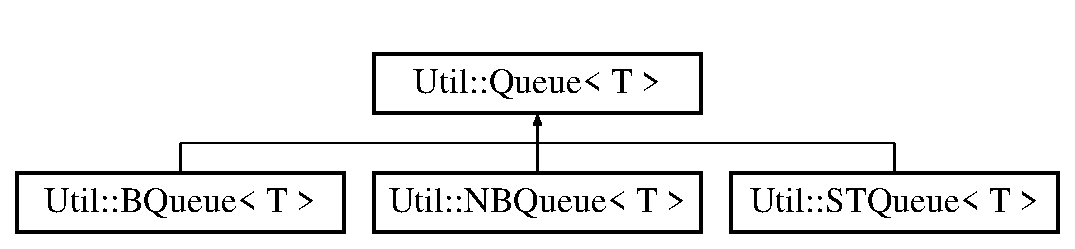
\includegraphics[height=2.000000cm]{class_util_1_1_queue}
\end{center}
\end{figure}
\subsection*{Public Member Functions}
\begin{DoxyCompactItemize}
\item 
\mbox{\Hypertarget{class_util_1_1_queue_ac4496936a971174064269f542ff44c5a}\label{class_util_1_1_queue_ac4496936a971174064269f542ff44c5a}} 
virtual T {\bfseries pop} ()=0
\item 
\mbox{\Hypertarget{class_util_1_1_queue_ab201f265252a832dd3629ba53af5a8b9}\label{class_util_1_1_queue_ab201f265252a832dd3629ba53af5a8b9}} 
virtual void {\bfseries push} (T t)=0
\item 
\mbox{\Hypertarget{class_util_1_1_queue_a7ecc9dbe7c52f9f49a575d43ff8cc583}\label{class_util_1_1_queue_a7ecc9dbe7c52f9f49a575d43ff8cc583}} 
virtual int {\bfseries size} ()=0
\end{DoxyCompactItemize}


The documentation for this class was generated from the following file\+:\begin{DoxyCompactItemize}
\item 
util/queue/Queue.\+h\end{DoxyCompactItemize}

\hypertarget{class_util_1_1_serialize}{}\section{Util\+:\+:Serialize Class Reference}
\label{class_util_1_1_serialize}\index{Util\+::\+Serialize@{Util\+::\+Serialize}}
Inheritance diagram for Util\+:\+:Serialize\+:\begin{figure}[H]
\begin{center}
\leavevmode
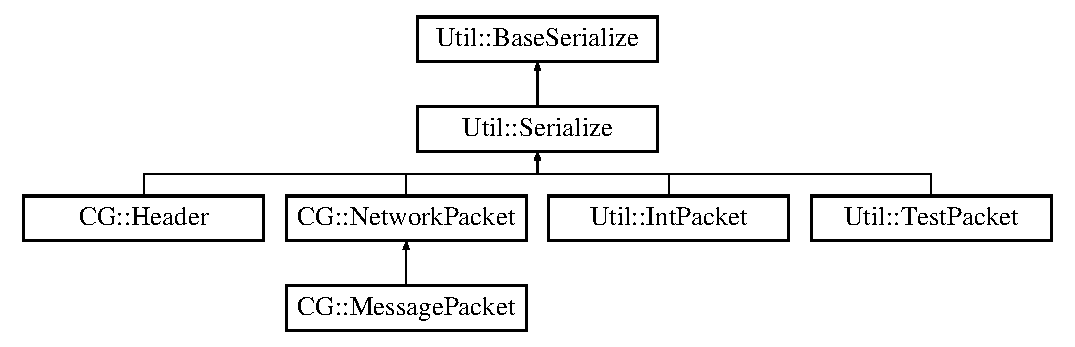
\includegraphics[height=4.000000cm]{class_util_1_1_serialize}
\end{center}
\end{figure}
\subsection*{Public Member Functions}
\begin{DoxyCompactItemize}
\item 
\mbox{\Hypertarget{class_util_1_1_serialize_ac0c8ca22862300a3ac5ac2e62775026d}\label{class_util_1_1_serialize_ac0c8ca22862300a3ac5ac2e62775026d}} 
void {\bfseries add\+Member\+Value} (int16\+\_\+t $\ast$value)
\item 
\mbox{\Hypertarget{class_util_1_1_serialize_af32004049863564d93552342f8c86c12}\label{class_util_1_1_serialize_af32004049863564d93552342f8c86c12}} 
void {\bfseries add\+Member\+Value} (int32\+\_\+t $\ast$value)
\item 
\mbox{\Hypertarget{class_util_1_1_serialize_acece47eb3acbc539a754286970620926}\label{class_util_1_1_serialize_acece47eb3acbc539a754286970620926}} 
void {\bfseries add\+Member\+Value} (int64\+\_\+t $\ast$value)
\item 
\mbox{\Hypertarget{class_util_1_1_serialize_a50529f4faceffd3c920eaf6119707004}\label{class_util_1_1_serialize_a50529f4faceffd3c920eaf6119707004}} 
void {\bfseries add\+Member\+Value} (std\+::string $\ast$value)
\item 
\mbox{\Hypertarget{class_util_1_1_serialize_a45fb568149d14fde53fdafaa04bf26b5}\label{class_util_1_1_serialize_a45fb568149d14fde53fdafaa04bf26b5}} 
void {\bfseries add\+Member\+Value} (\mbox{\hyperlink{class_util_1_1_serialize}{Serialize}} $\ast$value)
\item 
\mbox{\Hypertarget{class_util_1_1_serialize_a1ceca1091b0f879863624bb33edb3e3a}\label{class_util_1_1_serialize_a1ceca1091b0f879863624bb33edb3e3a}} 
void {\bfseries add\+Member\+Value} (std\+::list$<$ int32\+\_\+t $>$ $\ast$value)
\item 
\mbox{\Hypertarget{class_util_1_1_serialize_a9fc7588f3d13468421eabde95e725200}\label{class_util_1_1_serialize_a9fc7588f3d13468421eabde95e725200}} 
void {\bfseries add\+Member\+Value} (std\+::list$<$ \mbox{\hyperlink{class_util_1_1_serialize}{Serialize}} $\ast$$>$ $\ast$value)
\item 
int \mbox{\hyperlink{class_util_1_1_serialize_ae845c43beb63dddca9cf9fd26b39985d}{serialize}} (char $\ast$data)
\begin{DoxyCompactList}\small\item\em �޼��� ���� ���� \end{DoxyCompactList}\item 
\mbox{\Hypertarget{class_util_1_1_serialize_a0b0670440b6dd0a02b2060fb5cfde2a2}\label{class_util_1_1_serialize_a0b0670440b6dd0a02b2060fb5cfde2a2}} 
int {\bfseries deserialize} (const char $\ast$data)
\item 
\mbox{\Hypertarget{class_util_1_1_serialize_a95cc1c91dc5e8447d654c5a885db5823}\label{class_util_1_1_serialize_a95cc1c91dc5e8447d654c5a885db5823}} 
int {\bfseries size} ()
\end{DoxyCompactItemize}


\subsection{Member Function Documentation}
\mbox{\Hypertarget{class_util_1_1_serialize_ae845c43beb63dddca9cf9fd26b39985d}\label{class_util_1_1_serialize_ae845c43beb63dddca9cf9fd26b39985d}} 
\index{Util\+::\+Serialize@{Util\+::\+Serialize}!serialize@{serialize}}
\index{serialize@{serialize}!Util\+::\+Serialize@{Util\+::\+Serialize}}
\subsubsection{\texorpdfstring{serialize()}{serialize()}}
{\footnotesize\ttfamily int Util\+::\+Serialize\+::serialize (\begin{DoxyParamCaption}\item[{char $\ast$}]{data }\end{DoxyParamCaption})\hspace{0.3cm}{\ttfamily [virtual]}}



�޼��� ���� ���� 


\begin{DoxyParams}{Parameters}
{\em string} & a �Ķ���� �� \\
\hline
{\em string} & b \\
\hline
\end{DoxyParams}
\begin{DoxyReturn}{Returns}
mixed$\vert$boolean 
\end{DoxyReturn}


Implements \mbox{\hyperlink{class_util_1_1_base_serialize_ad85061a66f46acebc8457b88d971e022}{Util\+::\+Base\+Serialize}}.



The documentation for this class was generated from the following files\+:\begin{DoxyCompactItemize}
\item 
util/serialize/Serialize.\+h\item 
util/serialize/Serialize.\+cpp\end{DoxyCompactItemize}

\hypertarget{class_util_1_1_serialize_int16}{}\section{Util\+:\+:Serialize\+Int16 Class Reference}
\label{class_util_1_1_serialize_int16}\index{Util\+::\+Serialize\+Int16@{Util\+::\+Serialize\+Int16}}
Inheritance diagram for Util\+:\+:Serialize\+Int16\+:\begin{figure}[H]
\begin{center}
\leavevmode
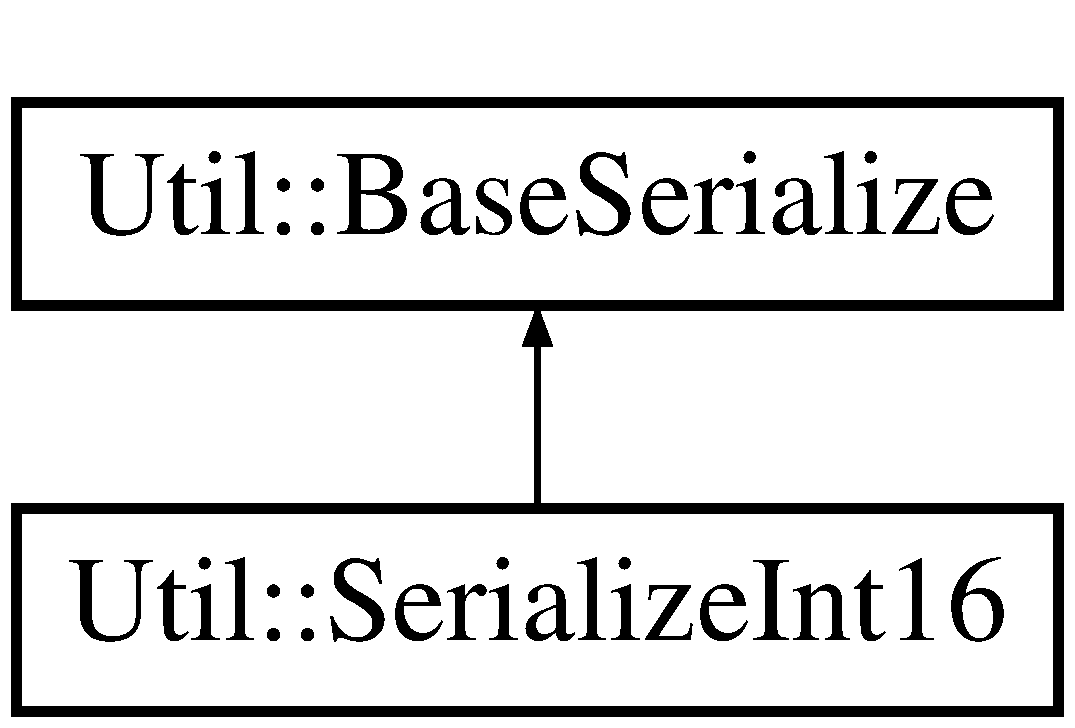
\includegraphics[height=2.000000cm]{class_util_1_1_serialize_int16}
\end{center}
\end{figure}
\subsection*{Public Member Functions}
\begin{DoxyCompactItemize}
\item 
\mbox{\Hypertarget{class_util_1_1_serialize_int16_a5002d2714a0f9a5913c899b58093e80d}\label{class_util_1_1_serialize_int16_a5002d2714a0f9a5913c899b58093e80d}} 
{\bfseries Serialize\+Int16} (int16\+\_\+t $\ast$p\+Value)
\item 
int \mbox{\hyperlink{class_util_1_1_serialize_int16_aee385ff01c25dbaf72c5da98d8dbc229}{serialize}} (char $\ast$data)
\begin{DoxyCompactList}\small\item\em �޼��� ���� ���� \end{DoxyCompactList}\item 
\mbox{\Hypertarget{class_util_1_1_serialize_int16_a96739e6e76aa2da346f3f6eceb772cad}\label{class_util_1_1_serialize_int16_a96739e6e76aa2da346f3f6eceb772cad}} 
int {\bfseries deserialize} (const char $\ast$data)
\item 
\mbox{\Hypertarget{class_util_1_1_serialize_int16_a49ca17322294ac997ac8820cfa15043e}\label{class_util_1_1_serialize_int16_a49ca17322294ac997ac8820cfa15043e}} 
int {\bfseries size} ()
\end{DoxyCompactItemize}


\subsection{Member Function Documentation}
\mbox{\Hypertarget{class_util_1_1_serialize_int16_aee385ff01c25dbaf72c5da98d8dbc229}\label{class_util_1_1_serialize_int16_aee385ff01c25dbaf72c5da98d8dbc229}} 
\index{Util\+::\+Serialize\+Int16@{Util\+::\+Serialize\+Int16}!serialize@{serialize}}
\index{serialize@{serialize}!Util\+::\+Serialize\+Int16@{Util\+::\+Serialize\+Int16}}
\subsubsection{\texorpdfstring{serialize()}{serialize()}}
{\footnotesize\ttfamily int Util\+::\+Serialize\+Int16\+::serialize (\begin{DoxyParamCaption}\item[{char $\ast$}]{data }\end{DoxyParamCaption})\hspace{0.3cm}{\ttfamily [virtual]}}



�޼��� ���� ���� 


\begin{DoxyParams}{Parameters}
{\em string} & a �Ķ���� �� \\
\hline
{\em string} & b \\
\hline
\end{DoxyParams}
\begin{DoxyReturn}{Returns}
mixed$\vert$boolean 
\end{DoxyReturn}


Implements \mbox{\hyperlink{class_util_1_1_base_serialize_ad85061a66f46acebc8457b88d971e022}{Util\+::\+Base\+Serialize}}.



The documentation for this class was generated from the following files\+:\begin{DoxyCompactItemize}
\item 
util/serialize/Serialize.\+h\item 
util/serialize/Serialize.\+cpp\end{DoxyCompactItemize}

\hypertarget{class_util_1_1_serialize_int32}{}\section{Util\+:\+:Serialize\+Int32 Class Reference}
\label{class_util_1_1_serialize_int32}\index{Util\+::\+Serialize\+Int32@{Util\+::\+Serialize\+Int32}}
Inheritance diagram for Util\+:\+:Serialize\+Int32\+:\begin{figure}[H]
\begin{center}
\leavevmode
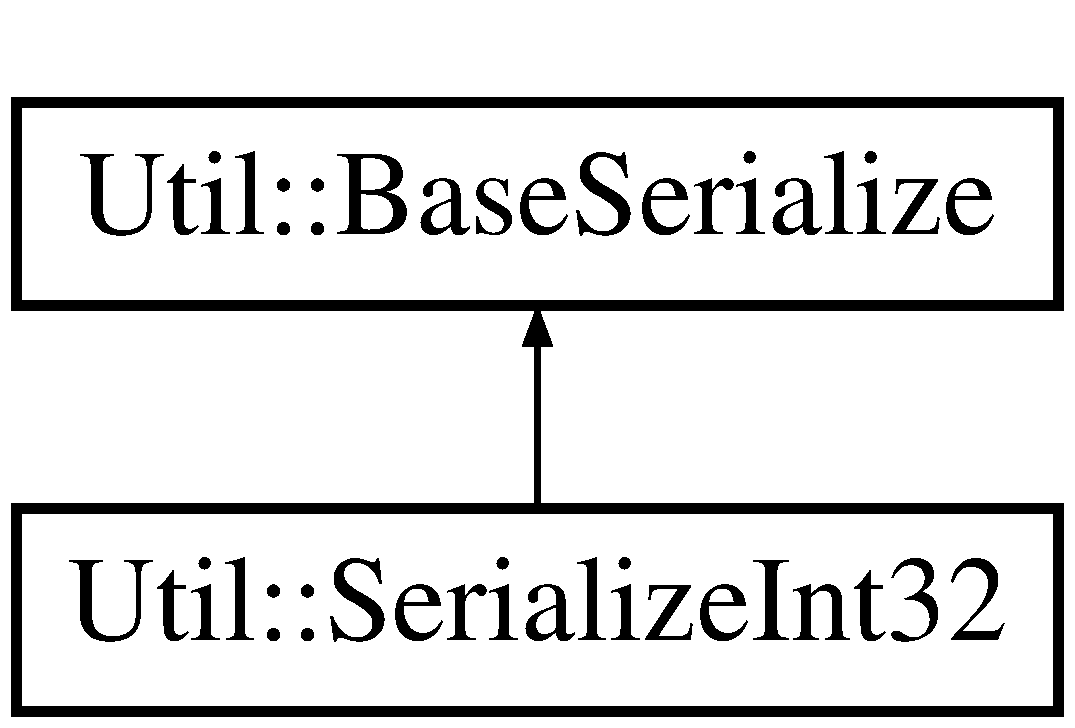
\includegraphics[height=2.000000cm]{class_util_1_1_serialize_int32}
\end{center}
\end{figure}
\subsection*{Public Member Functions}
\begin{DoxyCompactItemize}
\item 
\mbox{\Hypertarget{class_util_1_1_serialize_int32_aad551bded2bde82437f993697728f136}\label{class_util_1_1_serialize_int32_aad551bded2bde82437f993697728f136}} 
{\bfseries Serialize\+Int32} (int32\+\_\+t $\ast$p\+Value)
\item 
int \mbox{\hyperlink{class_util_1_1_serialize_int32_ae0472419db7afe580206f8498d99c447}{serialize}} (char $\ast$data)
\begin{DoxyCompactList}\small\item\em �޼��� ���� ���� \end{DoxyCompactList}\item 
\mbox{\Hypertarget{class_util_1_1_serialize_int32_ab528f6cac4e0e9241d7c762c950195b4}\label{class_util_1_1_serialize_int32_ab528f6cac4e0e9241d7c762c950195b4}} 
int {\bfseries deserialize} (const char $\ast$data)
\item 
\mbox{\Hypertarget{class_util_1_1_serialize_int32_a968e2d2dc375fdc1ba20b40ce4599e09}\label{class_util_1_1_serialize_int32_a968e2d2dc375fdc1ba20b40ce4599e09}} 
int {\bfseries size} ()
\end{DoxyCompactItemize}


\subsection{Member Function Documentation}
\mbox{\Hypertarget{class_util_1_1_serialize_int32_ae0472419db7afe580206f8498d99c447}\label{class_util_1_1_serialize_int32_ae0472419db7afe580206f8498d99c447}} 
\index{Util\+::\+Serialize\+Int32@{Util\+::\+Serialize\+Int32}!serialize@{serialize}}
\index{serialize@{serialize}!Util\+::\+Serialize\+Int32@{Util\+::\+Serialize\+Int32}}
\subsubsection{\texorpdfstring{serialize()}{serialize()}}
{\footnotesize\ttfamily int Util\+::\+Serialize\+Int32\+::serialize (\begin{DoxyParamCaption}\item[{char $\ast$}]{data }\end{DoxyParamCaption})\hspace{0.3cm}{\ttfamily [virtual]}}



�޼��� ���� ���� 


\begin{DoxyParams}{Parameters}
{\em string} & a �Ķ���� �� \\
\hline
{\em string} & b \\
\hline
\end{DoxyParams}
\begin{DoxyReturn}{Returns}
mixed$\vert$boolean 
\end{DoxyReturn}


Implements \mbox{\hyperlink{class_util_1_1_base_serialize_ad85061a66f46acebc8457b88d971e022}{Util\+::\+Base\+Serialize}}.



The documentation for this class was generated from the following files\+:\begin{DoxyCompactItemize}
\item 
util/serialize/Serialize.\+h\item 
util/serialize/Serialize.\+cpp\end{DoxyCompactItemize}

\hypertarget{class_util_1_1_serialize_int32_list}{}\section{Util\+:\+:Serialize\+Int32\+List Class Reference}
\label{class_util_1_1_serialize_int32_list}\index{Util\+::\+Serialize\+Int32\+List@{Util\+::\+Serialize\+Int32\+List}}
Inheritance diagram for Util\+:\+:Serialize\+Int32\+List\+:\begin{figure}[H]
\begin{center}
\leavevmode
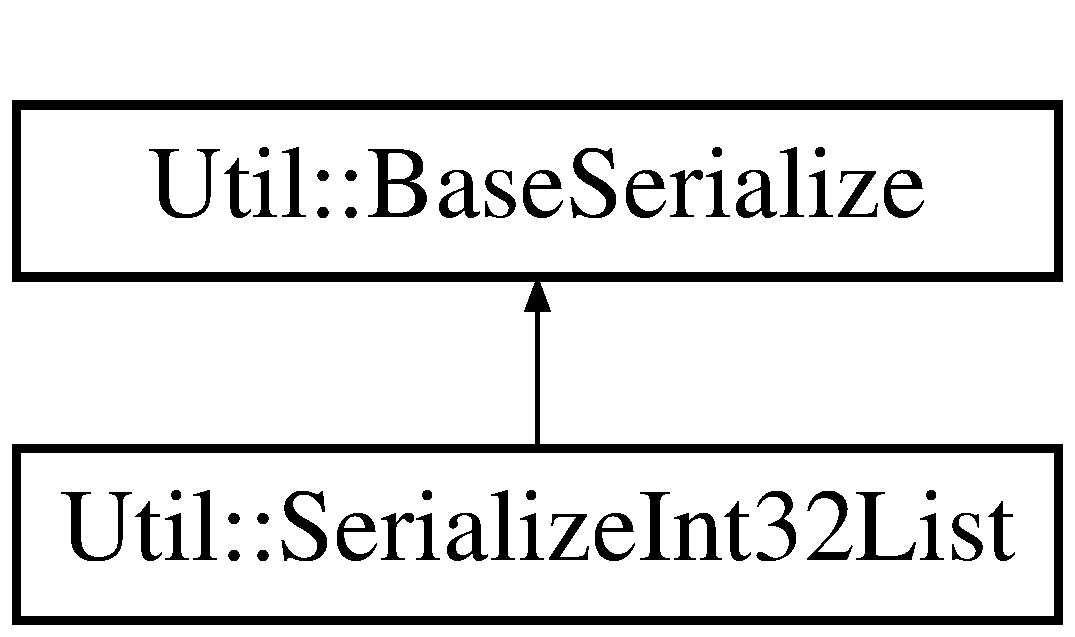
\includegraphics[height=2.000000cm]{class_util_1_1_serialize_int32_list}
\end{center}
\end{figure}
\subsection*{Public Member Functions}
\begin{DoxyCompactItemize}
\item 
\mbox{\Hypertarget{class_util_1_1_serialize_int32_list_a8302eba8ee52581e78a13175c21f60f2}\label{class_util_1_1_serialize_int32_list_a8302eba8ee52581e78a13175c21f60f2}} 
{\bfseries Serialize\+Int32\+List} (std\+::list$<$ int32\+\_\+t $>$ $\ast$p\+Value\+List)
\item 
int \mbox{\hyperlink{class_util_1_1_serialize_int32_list_a483adaa0778302e7a3ba86a3e7d23618}{serialize}} (char $\ast$data)
\begin{DoxyCompactList}\small\item\em �޼��� ���� ���� \end{DoxyCompactList}\item 
\mbox{\Hypertarget{class_util_1_1_serialize_int32_list_a7d764d0b6d277f74ba774645d867cc39}\label{class_util_1_1_serialize_int32_list_a7d764d0b6d277f74ba774645d867cc39}} 
int {\bfseries deserialize} (const char $\ast$data)
\item 
\mbox{\Hypertarget{class_util_1_1_serialize_int32_list_a5ed6c6a935358fd56d68bed3992a9aa8}\label{class_util_1_1_serialize_int32_list_a5ed6c6a935358fd56d68bed3992a9aa8}} 
int {\bfseries size} ()
\end{DoxyCompactItemize}


\subsection{Member Function Documentation}
\mbox{\Hypertarget{class_util_1_1_serialize_int32_list_a483adaa0778302e7a3ba86a3e7d23618}\label{class_util_1_1_serialize_int32_list_a483adaa0778302e7a3ba86a3e7d23618}} 
\index{Util\+::\+Serialize\+Int32\+List@{Util\+::\+Serialize\+Int32\+List}!serialize@{serialize}}
\index{serialize@{serialize}!Util\+::\+Serialize\+Int32\+List@{Util\+::\+Serialize\+Int32\+List}}
\subsubsection{\texorpdfstring{serialize()}{serialize()}}
{\footnotesize\ttfamily int Util\+::\+Serialize\+Int32\+List\+::serialize (\begin{DoxyParamCaption}\item[{char $\ast$}]{data }\end{DoxyParamCaption})\hspace{0.3cm}{\ttfamily [virtual]}}



�޼��� ���� ���� 


\begin{DoxyParams}{Parameters}
{\em string} & a �Ķ���� �� \\
\hline
{\em string} & b \\
\hline
\end{DoxyParams}
\begin{DoxyReturn}{Returns}
mixed$\vert$boolean 
\end{DoxyReturn}


Implements \mbox{\hyperlink{class_util_1_1_base_serialize_ad85061a66f46acebc8457b88d971e022}{Util\+::\+Base\+Serialize}}.



The documentation for this class was generated from the following files\+:\begin{DoxyCompactItemize}
\item 
util/serialize/Serialize.\+h\item 
util/serialize/Serialize.\+cpp\end{DoxyCompactItemize}

\hypertarget{class_util_1_1_serialize_int64}{}\section{Util\+:\+:Serialize\+Int64 Class Reference}
\label{class_util_1_1_serialize_int64}\index{Util\+::\+Serialize\+Int64@{Util\+::\+Serialize\+Int64}}
Inheritance diagram for Util\+:\+:Serialize\+Int64\+:\begin{figure}[H]
\begin{center}
\leavevmode
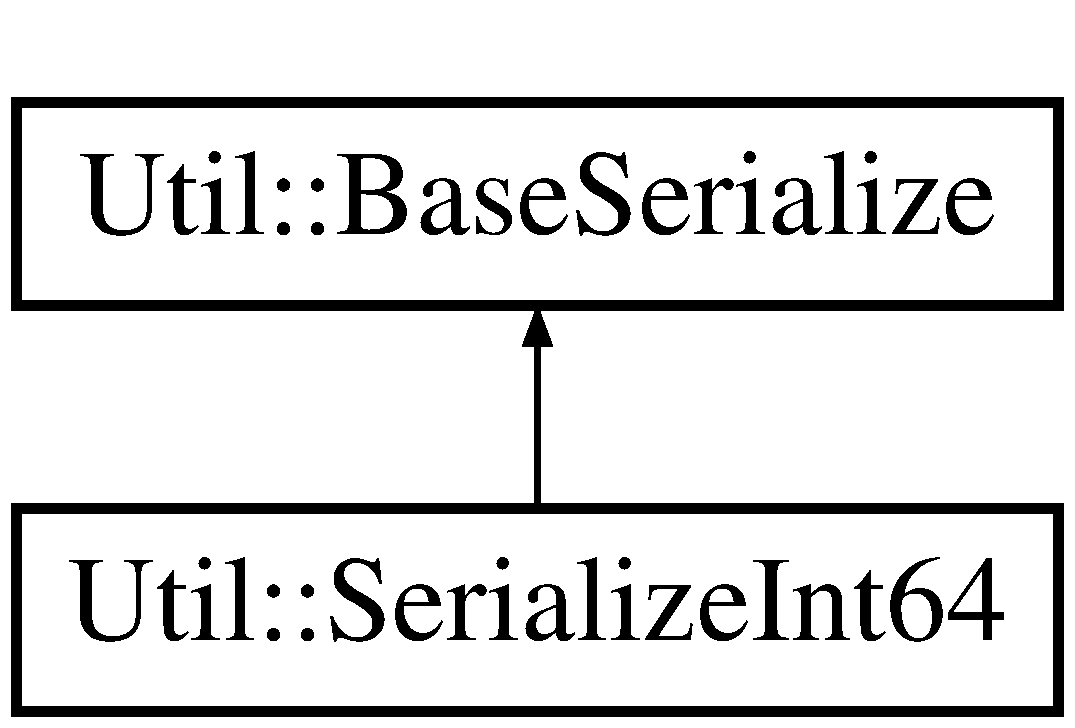
\includegraphics[height=2.000000cm]{class_util_1_1_serialize_int64}
\end{center}
\end{figure}
\subsection*{Public Member Functions}
\begin{DoxyCompactItemize}
\item 
\mbox{\Hypertarget{class_util_1_1_serialize_int64_ae05e80d377e865b2b200f16daa8df7b1}\label{class_util_1_1_serialize_int64_ae05e80d377e865b2b200f16daa8df7b1}} 
{\bfseries Serialize\+Int64} (int64\+\_\+t $\ast$p\+Value)
\item 
int \mbox{\hyperlink{class_util_1_1_serialize_int64_ad25b7294bd4ef93ab71377f508534413}{serialize}} (char $\ast$data)
\begin{DoxyCompactList}\small\item\em �޼��� ���� ���� \end{DoxyCompactList}\item 
\mbox{\Hypertarget{class_util_1_1_serialize_int64_add9f38784d1aee4362b9260df39a994d}\label{class_util_1_1_serialize_int64_add9f38784d1aee4362b9260df39a994d}} 
int {\bfseries deserialize} (const char $\ast$data)
\item 
\mbox{\Hypertarget{class_util_1_1_serialize_int64_a3889179d1616f07ab83d186800fcb6b6}\label{class_util_1_1_serialize_int64_a3889179d1616f07ab83d186800fcb6b6}} 
int {\bfseries size} ()
\end{DoxyCompactItemize}


\subsection{Member Function Documentation}
\mbox{\Hypertarget{class_util_1_1_serialize_int64_ad25b7294bd4ef93ab71377f508534413}\label{class_util_1_1_serialize_int64_ad25b7294bd4ef93ab71377f508534413}} 
\index{Util\+::\+Serialize\+Int64@{Util\+::\+Serialize\+Int64}!serialize@{serialize}}
\index{serialize@{serialize}!Util\+::\+Serialize\+Int64@{Util\+::\+Serialize\+Int64}}
\subsubsection{\texorpdfstring{serialize()}{serialize()}}
{\footnotesize\ttfamily int Util\+::\+Serialize\+Int64\+::serialize (\begin{DoxyParamCaption}\item[{char $\ast$}]{data }\end{DoxyParamCaption})\hspace{0.3cm}{\ttfamily [virtual]}}



�޼��� ���� ���� 


\begin{DoxyParams}{Parameters}
{\em string} & a �Ķ���� �� \\
\hline
{\em string} & b \\
\hline
\end{DoxyParams}
\begin{DoxyReturn}{Returns}
mixed$\vert$boolean 
\end{DoxyReturn}


Implements \mbox{\hyperlink{class_util_1_1_base_serialize_ad85061a66f46acebc8457b88d971e022}{Util\+::\+Base\+Serialize}}.



The documentation for this class was generated from the following files\+:\begin{DoxyCompactItemize}
\item 
util/serialize/Serialize.\+h\item 
util/serialize/Serialize.\+cpp\end{DoxyCompactItemize}

\hypertarget{class_util_1_1_serialize_string}{}\section{Util\+:\+:Serialize\+String Class Reference}
\label{class_util_1_1_serialize_string}\index{Util\+::\+Serialize\+String@{Util\+::\+Serialize\+String}}
Inheritance diagram for Util\+:\+:Serialize\+String\+:\begin{figure}[H]
\begin{center}
\leavevmode
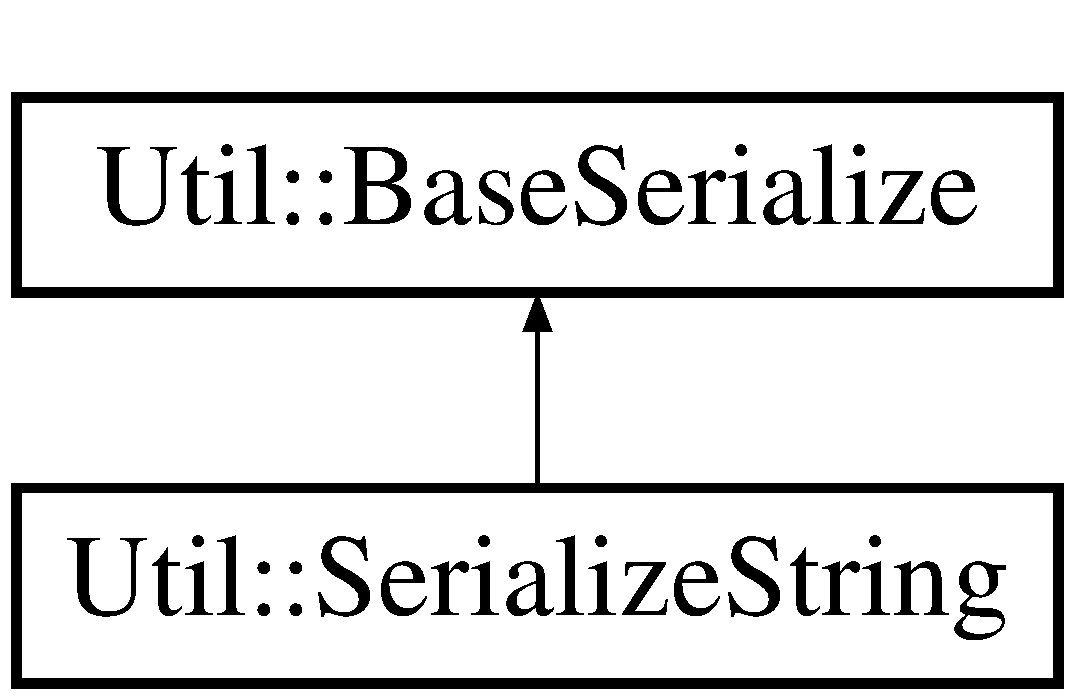
\includegraphics[height=2.000000cm]{class_util_1_1_serialize_string}
\end{center}
\end{figure}
\subsection*{Public Member Functions}
\begin{DoxyCompactItemize}
\item 
\mbox{\Hypertarget{class_util_1_1_serialize_string_abcce9818aeda60db4c265fde21af3b06}\label{class_util_1_1_serialize_string_abcce9818aeda60db4c265fde21af3b06}} 
{\bfseries Serialize\+String} (std\+::string $\ast$p\+Value)
\item 
int \mbox{\hyperlink{class_util_1_1_serialize_string_addaa66b71207e6e71a199ffbd0b0998f}{serialize}} (char $\ast$data)
\begin{DoxyCompactList}\small\item\em �޼��� ���� ���� \end{DoxyCompactList}\item 
\mbox{\Hypertarget{class_util_1_1_serialize_string_af9070d603baddd1145233086a2e4de2f}\label{class_util_1_1_serialize_string_af9070d603baddd1145233086a2e4de2f}} 
int {\bfseries deserialize} (const char $\ast$data)
\item 
\mbox{\Hypertarget{class_util_1_1_serialize_string_a8e921966bc9f299a80885ce38f5e78a0}\label{class_util_1_1_serialize_string_a8e921966bc9f299a80885ce38f5e78a0}} 
int {\bfseries size} ()
\end{DoxyCompactItemize}


\subsection{Member Function Documentation}
\mbox{\Hypertarget{class_util_1_1_serialize_string_addaa66b71207e6e71a199ffbd0b0998f}\label{class_util_1_1_serialize_string_addaa66b71207e6e71a199ffbd0b0998f}} 
\index{Util\+::\+Serialize\+String@{Util\+::\+Serialize\+String}!serialize@{serialize}}
\index{serialize@{serialize}!Util\+::\+Serialize\+String@{Util\+::\+Serialize\+String}}
\subsubsection{\texorpdfstring{serialize()}{serialize()}}
{\footnotesize\ttfamily int Util\+::\+Serialize\+String\+::serialize (\begin{DoxyParamCaption}\item[{char $\ast$}]{data }\end{DoxyParamCaption})\hspace{0.3cm}{\ttfamily [virtual]}}



�޼��� ���� ���� 


\begin{DoxyParams}{Parameters}
{\em string} & a �Ķ���� �� \\
\hline
{\em string} & b \\
\hline
\end{DoxyParams}
\begin{DoxyReturn}{Returns}
mixed$\vert$boolean 
\end{DoxyReturn}


Implements \mbox{\hyperlink{class_util_1_1_base_serialize_ad85061a66f46acebc8457b88d971e022}{Util\+::\+Base\+Serialize}}.



The documentation for this class was generated from the following files\+:\begin{DoxyCompactItemize}
\item 
util/serialize/Serialize.\+h\item 
util/serialize/Serialize.\+cpp\end{DoxyCompactItemize}

\hypertarget{class_c_g_1_1_server}{}\section{CG\+:\+:Server Class Reference}
\label{class_c_g_1_1_server}\index{C\+G\+::\+Server@{C\+G\+::\+Server}}
Inheritance diagram for CG\+:\+:Server\+:\begin{figure}[H]
\begin{center}
\leavevmode
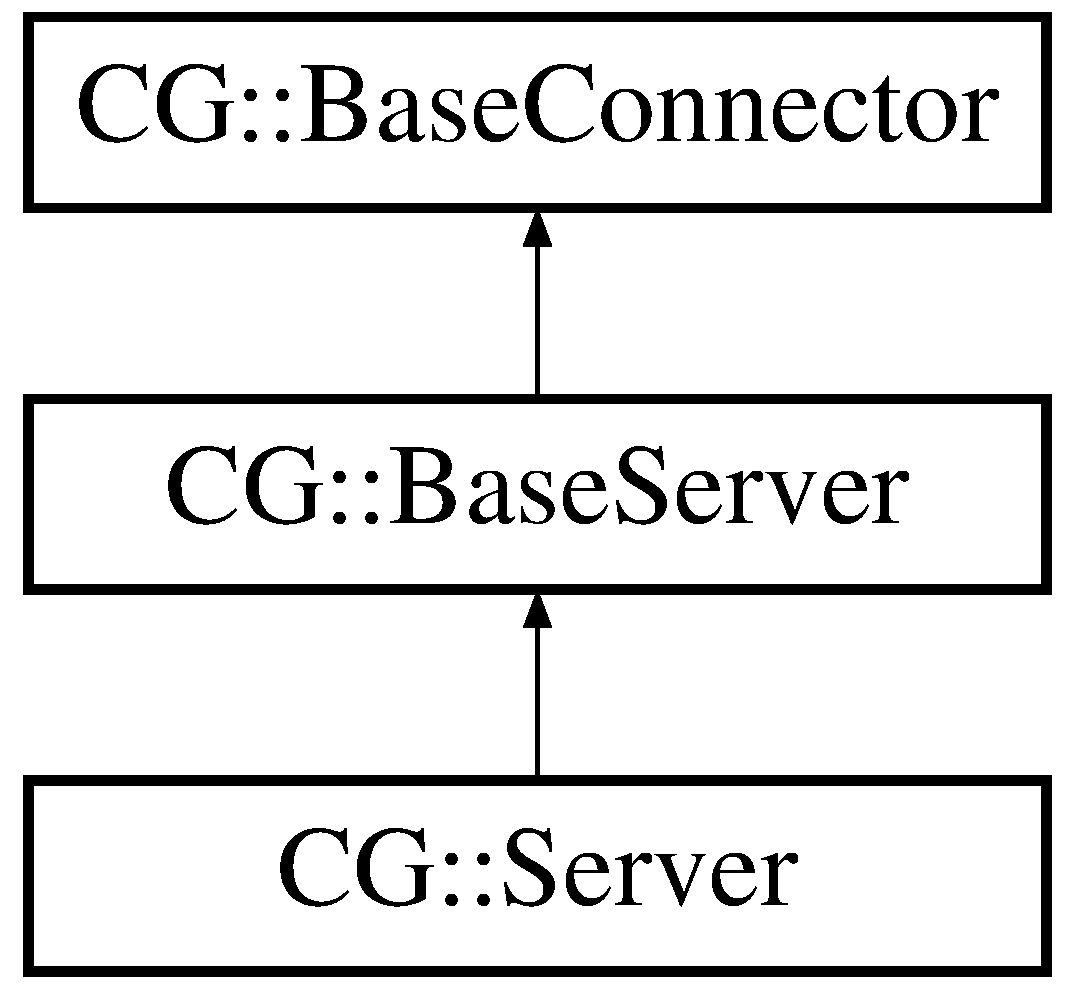
\includegraphics[height=3.000000cm]{class_c_g_1_1_server}
\end{center}
\end{figure}
\subsection*{Public Member Functions}
\begin{DoxyCompactItemize}
\item 
int \mbox{\hyperlink{class_c_g_1_1_server_a846ff65e508699775c54a81091ec76a3}{process\+Data}} (\mbox{\hyperlink{class_c_g_1_1_connector_info}{Connector\+Info}} $\ast$\mbox{\hyperlink{class_c_g_1_1_base_connector_ae68321ba56404549f2e655238035ed8d}{connector\+Info}}, char $\ast$data, int data\+Size)
\begin{DoxyCompactList}\small\item\em network call this function when came receiving data from others \end{DoxyCompactList}\item 
\mbox{\Hypertarget{class_c_g_1_1_server_a3d662cb8806e3577402da3abdfc2e5cf}\label{class_c_g_1_1_server_a3d662cb8806e3577402da3abdfc2e5cf}} 
void {\bfseries send\+Message} (Host\+Id hostid, char $\ast$data, int data\+Size)
\item 
\mbox{\Hypertarget{class_c_g_1_1_server_a1ae5a22ee3d8a272c2903e53639f61c6}\label{class_c_g_1_1_server_a1ae5a22ee3d8a272c2903e53639f61c6}} 
void {\bfseries send\+Message} (Host\+Id host\+Id, std\+::string message)
\end{DoxyCompactItemize}
\subsection*{Public Attributes}
\begin{DoxyCompactItemize}
\item 
\mbox{\Hypertarget{class_c_g_1_1_server_a4c1f26594dc7c336ad2c8e85e1f47f1e}\label{class_c_g_1_1_server_a4c1f26594dc7c336ad2c8e85e1f47f1e}} 
std\+::function$<$ void(Host\+Id, char $\ast$, int)$>$ {\bfseries on\+Receive}
\item 
\mbox{\Hypertarget{class_c_g_1_1_server_aa120a84948312f9ea3931a9b8d2f004e}\label{class_c_g_1_1_server_aa120a84948312f9ea3931a9b8d2f004e}} 
\mbox{\hyperlink{class_c_g_1_1_network_handler}{Network\+Handler}} $\ast$ {\bfseries network\+Handler}
\end{DoxyCompactItemize}
\subsection*{Additional Inherited Members}


\subsection{Member Function Documentation}
\mbox{\Hypertarget{class_c_g_1_1_server_a846ff65e508699775c54a81091ec76a3}\label{class_c_g_1_1_server_a846ff65e508699775c54a81091ec76a3}} 
\index{C\+G\+::\+Server@{C\+G\+::\+Server}!process\+Data@{process\+Data}}
\index{process\+Data@{process\+Data}!C\+G\+::\+Server@{C\+G\+::\+Server}}
\subsubsection{\texorpdfstring{process\+Data()}{processData()}}
{\footnotesize\ttfamily int C\+G\+::\+Server\+::process\+Data (\begin{DoxyParamCaption}\item[{\mbox{\hyperlink{class_c_g_1_1_connector_info}{Connector\+Info}} $\ast$}]{connector\+Info,  }\item[{char $\ast$}]{data,  }\item[{int}]{data\+Size }\end{DoxyParamCaption})\hspace{0.3cm}{\ttfamily [virtual]}}



network call this function when came receiving data from others 

\begin{DoxyAuthor}{Author}
kim yong-\/chan 
\end{DoxyAuthor}
\begin{DoxyDate}{Date}
2018-\/09-\/08 
\end{DoxyDate}

\begin{DoxyParams}{Parameters}
{\em Connector\+Info$\ast$} & connector\+Info \+: infomation who send data \\
\hline
{\em char$\ast$} & data \+: receive data from other \\
\hline
{\em int} & data\+Size \+: receive data size \\
\hline
\end{DoxyParams}
\begin{DoxyReturn}{Returns}
int index \+: if data doesn\textquotesingle{}t come all, return 0. if data is not correct, return nagative number. if data come perfect, return data size 
\end{DoxyReturn}


Implements \mbox{\hyperlink{class_c_g_1_1_base_connector_adf8eae41d668ead0f14e7f86b3cea825}{C\+G\+::\+Base\+Connector}}.



The documentation for this class was generated from the following files\+:\begin{DoxyCompactItemize}
\item 
network/module/basic/Server.\+h\item 
network/module/basic/Server.\+cpp\end{DoxyCompactItemize}

\hypertarget{class_c_g_1_1_server_config}{}\section{CG\+:\+:Server\+Config Class Reference}
\label{class_c_g_1_1_server_config}\index{C\+G\+::\+Server\+Config@{C\+G\+::\+Server\+Config}}


it is client config. same with connect\+Config but it will storage additional server infomation later  




{\ttfamily \#include $<$Base\+Server.\+h$>$}

Inheritance diagram for CG\+:\+:Server\+Config\+:\begin{figure}[H]
\begin{center}
\leavevmode
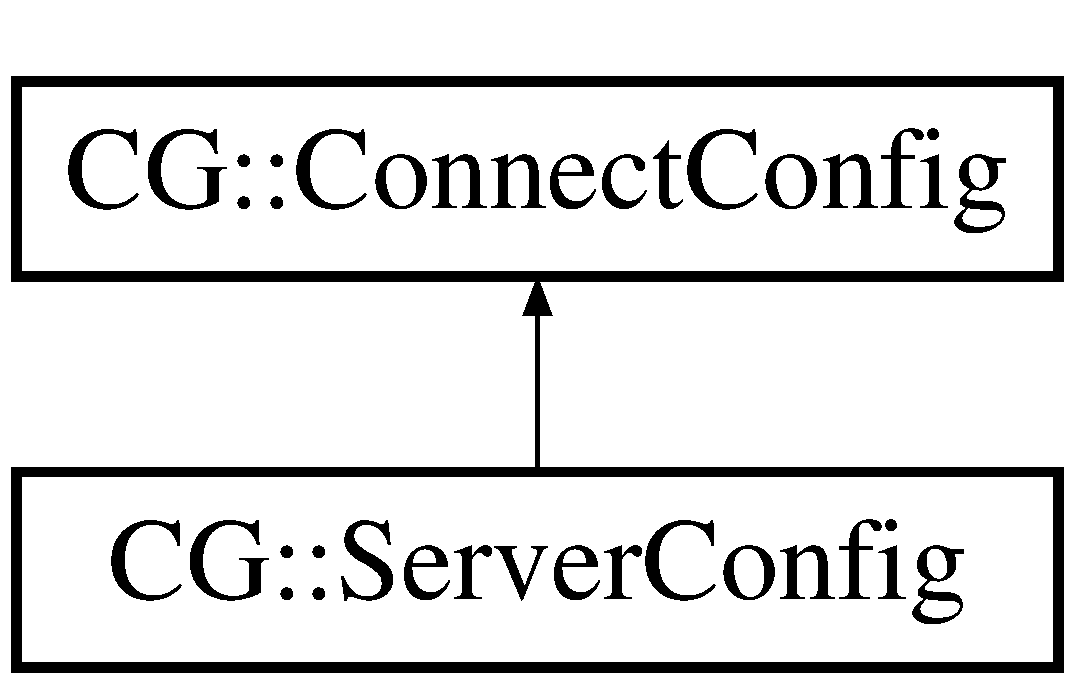
\includegraphics[height=2.000000cm]{class_c_g_1_1_server_config}
\end{center}
\end{figure}
\subsection*{Additional Inherited Members}


\subsection{Detailed Description}
it is client config. same with connect\+Config but it will storage additional server infomation later 

\begin{DoxyAuthor}{Author}
kim yong-\/chan 
\end{DoxyAuthor}
\begin{DoxyDate}{Date}
2018-\/09-\/08 
\end{DoxyDate}


The documentation for this class was generated from the following file\+:\begin{DoxyCompactItemize}
\item 
network/core/Base\+Server.\+h\end{DoxyCompactItemize}

\hypertarget{class_util_1_1_singleton}{}\section{Util\+:\+:Singleton$<$ T $>$ Class Template Reference}
\label{class_util_1_1_singleton}\index{Util\+::\+Singleton$<$ T $>$@{Util\+::\+Singleton$<$ T $>$}}
\subsection*{Static Public Member Functions}
\begin{DoxyCompactItemize}
\item 
\mbox{\Hypertarget{class_util_1_1_singleton_a1e2fe8ce46d83833b2c7eb3d918ae4fb}\label{class_util_1_1_singleton_a1e2fe8ce46d83833b2c7eb3d918ae4fb}} 
static T $\ast$ {\bfseries Get\+Instance} ()
\item 
\mbox{\Hypertarget{class_util_1_1_singleton_a227b4fff4d5948838a519c66c1a480f5}\label{class_util_1_1_singleton_a227b4fff4d5948838a519c66c1a480f5}} 
static void {\bfseries Destroy\+Instance} ()
\end{DoxyCompactItemize}


The documentation for this class was generated from the following file\+:\begin{DoxyCompactItemize}
\item 
util/singleton/Singleton.\+h\end{DoxyCompactItemize}

\hypertarget{class_util_1_1_spin_lock}{}\section{Util\+:\+:Spin\+Lock Class Reference}
\label{class_util_1_1_spin_lock}\index{Util\+::\+Spin\+Lock@{Util\+::\+Spin\+Lock}}
Inheritance diagram for Util\+:\+:Spin\+Lock\+:\begin{figure}[H]
\begin{center}
\leavevmode
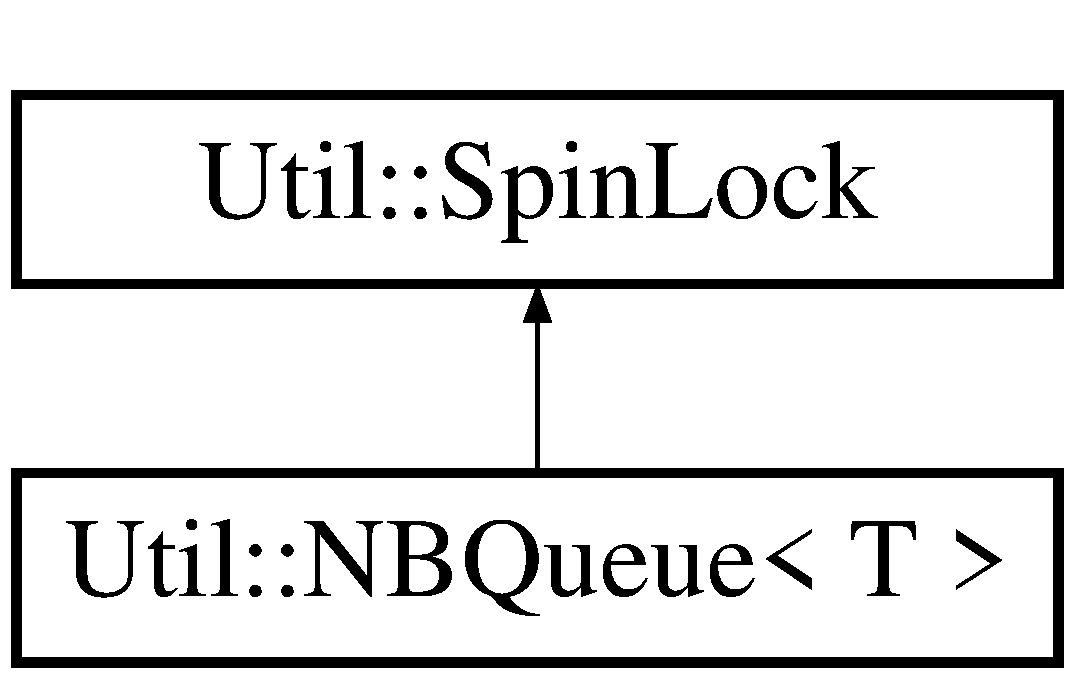
\includegraphics[height=2.000000cm]{class_util_1_1_spin_lock}
\end{center}
\end{figure}
\subsection*{Public Member Functions}
\begin{DoxyCompactItemize}
\item 
\mbox{\Hypertarget{class_util_1_1_spin_lock_a378ec825abf816959f51c9e68793a78b}\label{class_util_1_1_spin_lock_a378ec825abf816959f51c9e68793a78b}} 
void {\bfseries lock} ()
\item 
\mbox{\Hypertarget{class_util_1_1_spin_lock_a13079b44171b0b9750db9b20bb12933f}\label{class_util_1_1_spin_lock_a13079b44171b0b9750db9b20bb12933f}} 
void {\bfseries un\+Lock} ()
\end{DoxyCompactItemize}
\subsection*{Protected Attributes}
\begin{DoxyCompactItemize}
\item 
\mbox{\Hypertarget{class_util_1_1_spin_lock_a1db6f97fee8f6e37a89eba76b5d2dab5}\label{class_util_1_1_spin_lock_a1db6f97fee8f6e37a89eba76b5d2dab5}} 
std\+::mutex {\bfseries mutex}
\end{DoxyCompactItemize}


The documentation for this class was generated from the following file\+:\begin{DoxyCompactItemize}
\item 
util/lock/Spin\+Lock.\+h\end{DoxyCompactItemize}

\hypertarget{class_util_1_1_s_t_list}{}\section{Util\+:\+:S\+T\+List$<$ T $>$ Class Template Reference}
\label{class_util_1_1_s_t_list}\index{Util\+::\+S\+T\+List$<$ T $>$@{Util\+::\+S\+T\+List$<$ T $>$}}
Inheritance diagram for Util\+:\+:S\+T\+List$<$ T $>$\+:\begin{figure}[H]
\begin{center}
\leavevmode
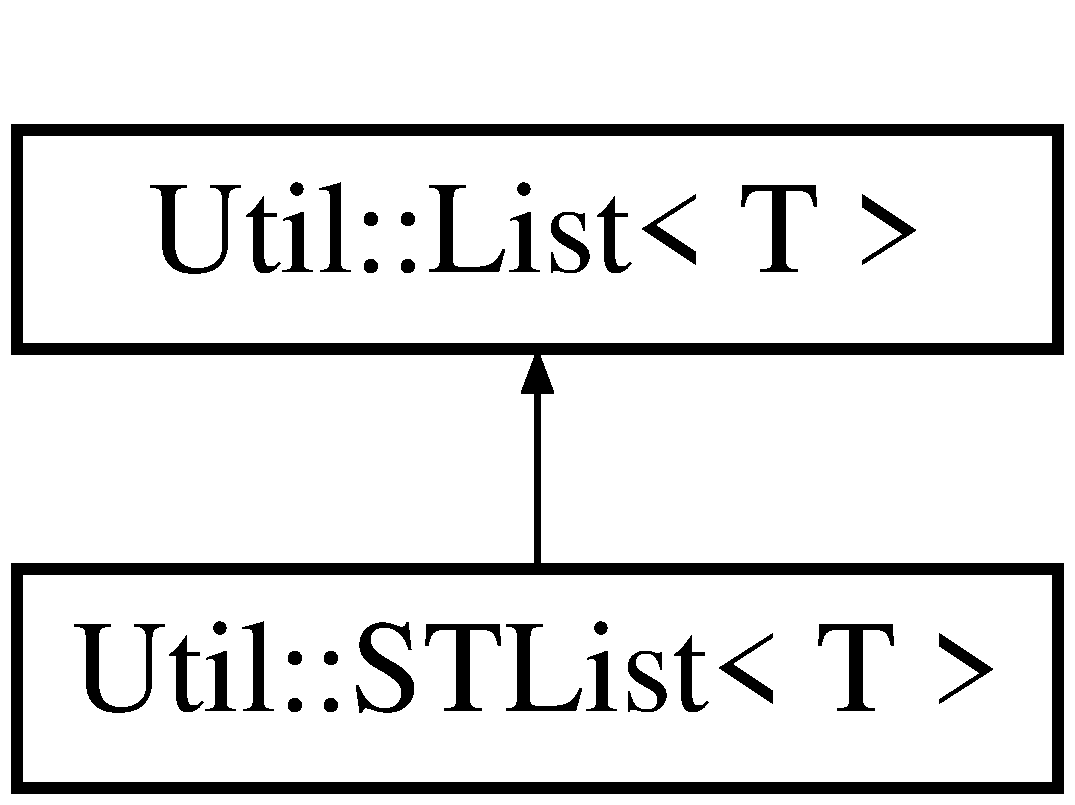
\includegraphics[height=2.000000cm]{class_util_1_1_s_t_list}
\end{center}
\end{figure}
\subsection*{Public Member Functions}
\begin{DoxyCompactItemize}
\item 
\mbox{\Hypertarget{class_util_1_1_s_t_list_a36b94b6bf675f12a3561c0d256c7e0de}\label{class_util_1_1_s_t_list_a36b94b6bf675f12a3561c0d256c7e0de}} 
T {\bfseries at} (int index)
\item 
\mbox{\Hypertarget{class_util_1_1_s_t_list_a58dc4769b737fa74d100ca0061504587}\label{class_util_1_1_s_t_list_a58dc4769b737fa74d100ca0061504587}} 
bool {\bfseries remove} (T t)
\item 
\mbox{\Hypertarget{class_util_1_1_s_t_list_a4bff8c08bb5c2299ffbf92be54eb5b42}\label{class_util_1_1_s_t_list_a4bff8c08bb5c2299ffbf92be54eb5b42}} 
bool {\bfseries remove} (int index)
\item 
\mbox{\Hypertarget{class_util_1_1_s_t_list_a117b785fc13aeaa4aaeaf292877d1823}\label{class_util_1_1_s_t_list_a117b785fc13aeaa4aaeaf292877d1823}} 
void {\bfseries push\+\_\+back} (T t)
\item 
\mbox{\Hypertarget{class_util_1_1_s_t_list_aa1193cc40023b76ddf6c158d63737994}\label{class_util_1_1_s_t_list_aa1193cc40023b76ddf6c158d63737994}} 
int {\bfseries size} ()
\end{DoxyCompactItemize}
\subsection*{Protected Attributes}
\begin{DoxyCompactItemize}
\item 
\mbox{\Hypertarget{class_util_1_1_s_t_list_ab9b34ca152516f0db1c212ce9ad1e9cf}\label{class_util_1_1_s_t_list_ab9b34ca152516f0db1c212ce9ad1e9cf}} 
std\+::vector$<$ T $>$ {\bfseries object\+List}
\end{DoxyCompactItemize}


The documentation for this class was generated from the following file\+:\begin{DoxyCompactItemize}
\item 
util/list/S\+T\+List.\+h\end{DoxyCompactItemize}

\hypertarget{class_util_1_1_s_t_queue}{}\section{Util\+:\+:S\+T\+Queue$<$ T $>$ Class Template Reference}
\label{class_util_1_1_s_t_queue}\index{Util\+::\+S\+T\+Queue$<$ T $>$@{Util\+::\+S\+T\+Queue$<$ T $>$}}
Inheritance diagram for Util\+:\+:S\+T\+Queue$<$ T $>$\+:\begin{figure}[H]
\begin{center}
\leavevmode
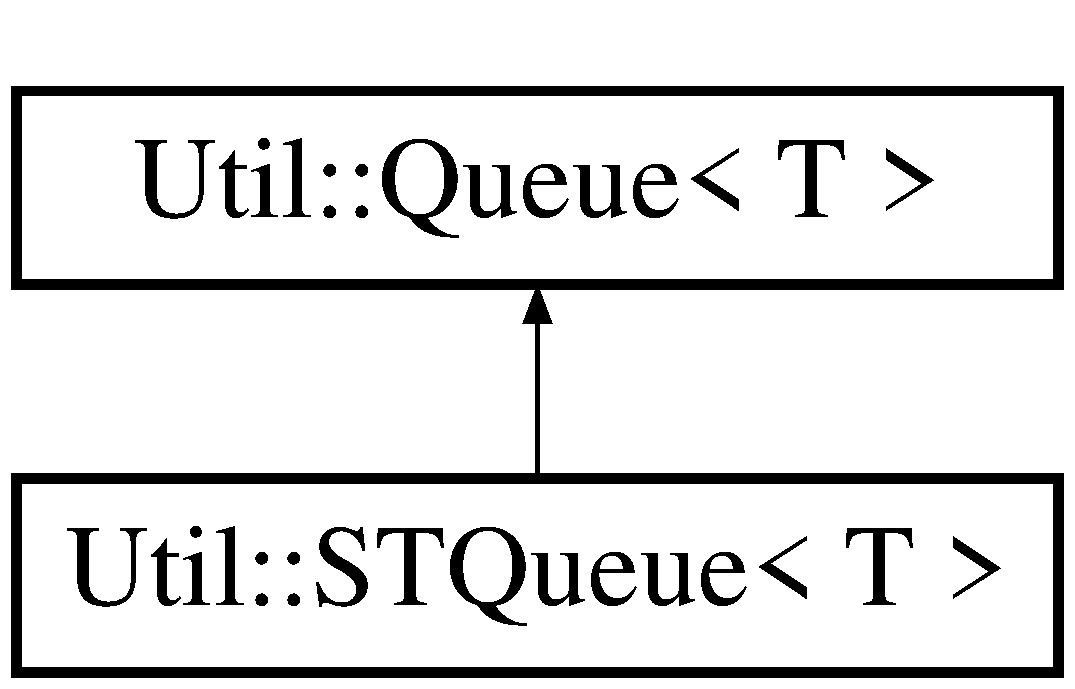
\includegraphics[height=2.000000cm]{class_util_1_1_s_t_queue}
\end{center}
\end{figure}
\subsection*{Public Member Functions}
\begin{DoxyCompactItemize}
\item 
\mbox{\Hypertarget{class_util_1_1_s_t_queue_a1e2f3196fbecf7944e019fb3deebb5a8}\label{class_util_1_1_s_t_queue_a1e2f3196fbecf7944e019fb3deebb5a8}} 
T {\bfseries pop} ()
\item 
\mbox{\Hypertarget{class_util_1_1_s_t_queue_a2cfc960d40efe8717d7ddca226e09425}\label{class_util_1_1_s_t_queue_a2cfc960d40efe8717d7ddca226e09425}} 
void {\bfseries push} (T t)
\item 
\mbox{\Hypertarget{class_util_1_1_s_t_queue_a2061e1db96e377c3721fe387c90f592c}\label{class_util_1_1_s_t_queue_a2061e1db96e377c3721fe387c90f592c}} 
int {\bfseries size} ()
\end{DoxyCompactItemize}
\subsection*{Protected Attributes}
\begin{DoxyCompactItemize}
\item 
\mbox{\Hypertarget{class_util_1_1_s_t_queue_a4dbd208b7093e61e55aeeebd724681b8}\label{class_util_1_1_s_t_queue_a4dbd208b7093e61e55aeeebd724681b8}} 
std\+::queue$<$ T $>$ {\bfseries object\+Queue}
\end{DoxyCompactItemize}


The documentation for this class was generated from the following file\+:\begin{DoxyCompactItemize}
\item 
util/queue/S\+T\+Queue.\+h\end{DoxyCompactItemize}

\hypertarget{class_util_1_1_test_packet}{}\section{Util\+:\+:Test\+Packet Class Reference}
\label{class_util_1_1_test_packet}\index{Util\+::\+Test\+Packet@{Util\+::\+Test\+Packet}}
Inheritance diagram for Util\+:\+:Test\+Packet\+:\begin{figure}[H]
\begin{center}
\leavevmode
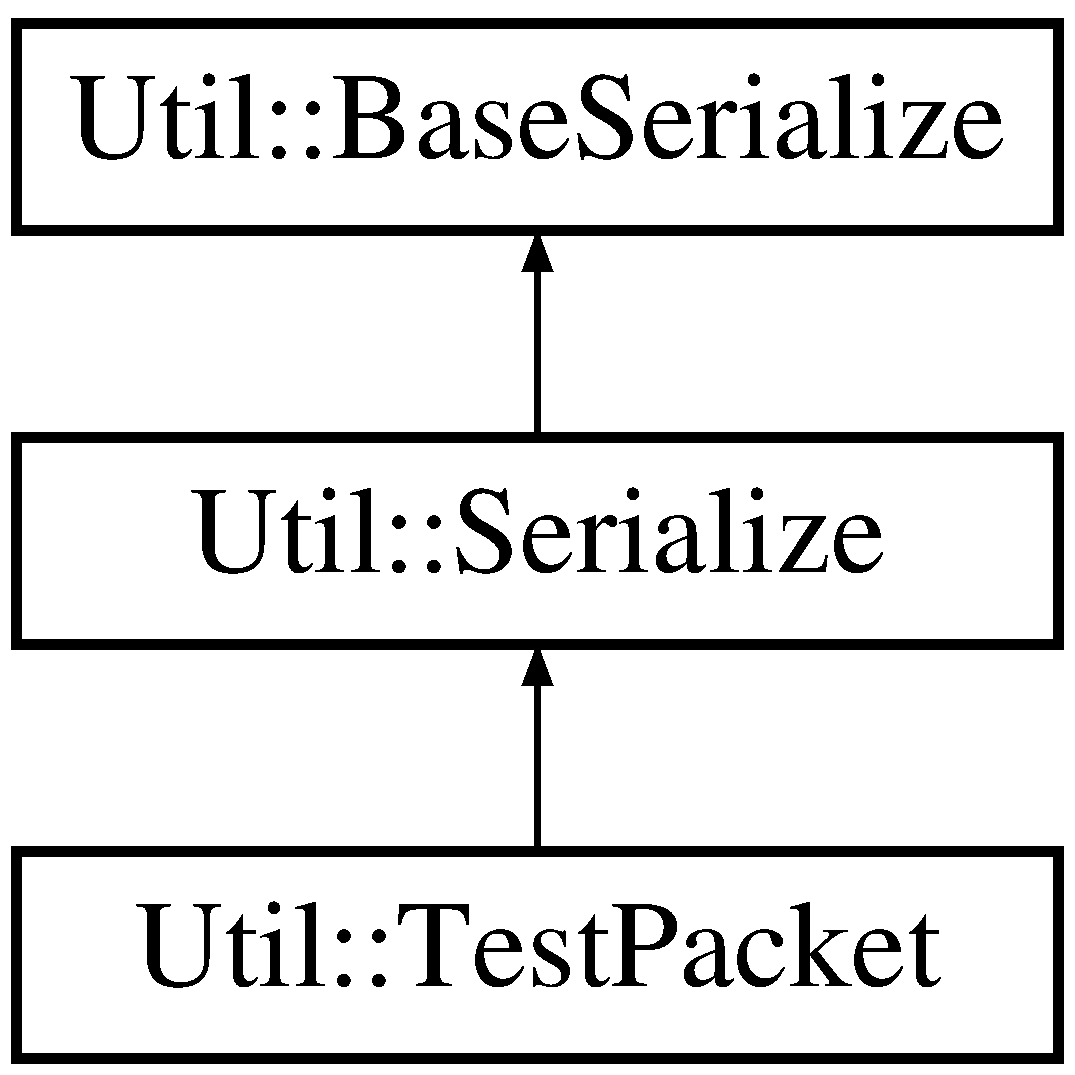
\includegraphics[height=3.000000cm]{class_util_1_1_test_packet}
\end{center}
\end{figure}
\subsection*{Public Attributes}
\begin{DoxyCompactItemize}
\item 
\mbox{\Hypertarget{class_util_1_1_test_packet_a560d8db6aef27b236679b3abc635fa5f}\label{class_util_1_1_test_packet_a560d8db6aef27b236679b3abc635fa5f}} 
int32\+\_\+t {\bfseries id1}
\item 
\mbox{\Hypertarget{class_util_1_1_test_packet_a4097111f98402d732af46a9f0720b04a}\label{class_util_1_1_test_packet_a4097111f98402d732af46a9f0720b04a}} 
int32\+\_\+t {\bfseries id2}
\item 
\mbox{\Hypertarget{class_util_1_1_test_packet_a3b85612effb996d70b095369ffb1eb5d}\label{class_util_1_1_test_packet_a3b85612effb996d70b095369ffb1eb5d}} 
\mbox{\hyperlink{class_util_1_1_int_packet}{Int\+Packet}} {\bfseries int\+Packet}
\item 
\mbox{\Hypertarget{class_util_1_1_test_packet_adf457e557b0b0a1fa7135e684a712362}\label{class_util_1_1_test_packet_adf457e557b0b0a1fa7135e684a712362}} 
std\+::list$<$ int32\+\_\+t $>$ {\bfseries test\+List}
\item 
\mbox{\Hypertarget{class_util_1_1_test_packet_aef391cb770445ef1581ed8e418da89e0}\label{class_util_1_1_test_packet_aef391cb770445ef1581ed8e418da89e0}} 
std\+::string {\bfseries str}
\end{DoxyCompactItemize}
\subsection*{Additional Inherited Members}


The documentation for this class was generated from the following file\+:\begin{DoxyCompactItemize}
\item 
util/serialize/Serialize.\+h\end{DoxyCompactItemize}

\hypertarget{class_util_1_1_thread}{}\section{Util\+:\+:Thread Class Reference}
\label{class_util_1_1_thread}\index{Util\+::\+Thread@{Util\+::\+Thread}}
Inheritance diagram for Util\+:\+:Thread\+:\begin{figure}[H]
\begin{center}
\leavevmode
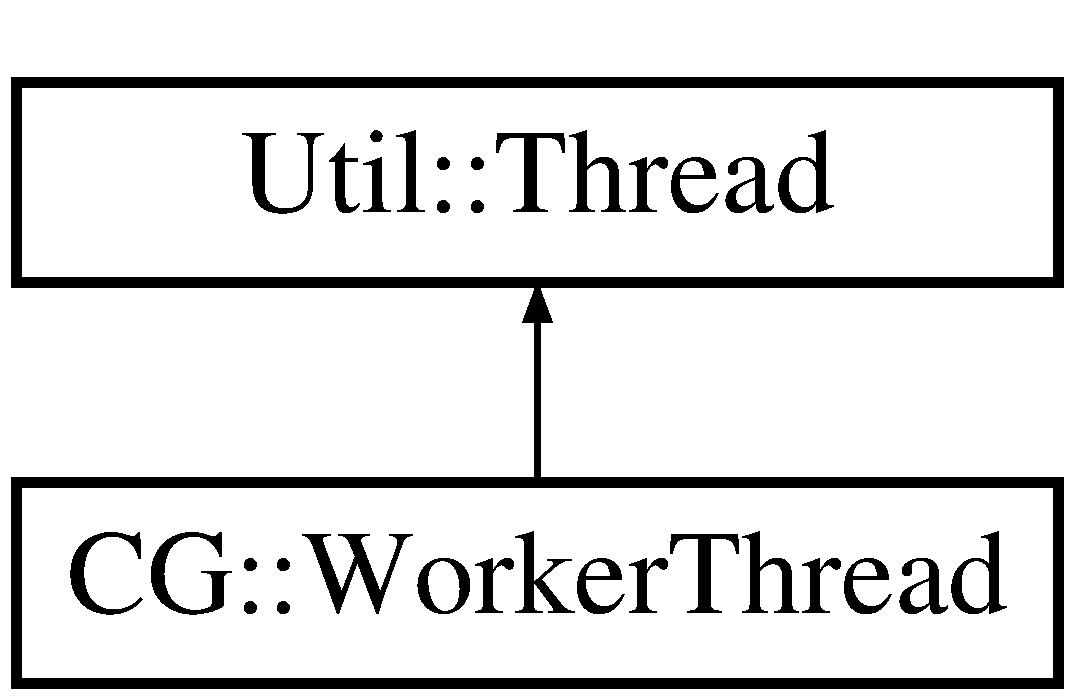
\includegraphics[height=2.000000cm]{class_util_1_1_thread}
\end{center}
\end{figure}
\subsection*{Public Member Functions}
\begin{DoxyCompactItemize}
\item 
\mbox{\Hypertarget{class_util_1_1_thread_a54459d58869864592196ae13aeb877ff}\label{class_util_1_1_thread_a54459d58869864592196ae13aeb877ff}} 
void {\bfseries start} ()
\item 
\mbox{\Hypertarget{class_util_1_1_thread_a6370a18a7409742671a1458fc0536f73}\label{class_util_1_1_thread_a6370a18a7409742671a1458fc0536f73}} 
void {\bfseries stop} ()
\item 
\mbox{\Hypertarget{class_util_1_1_thread_a03b356f7fa0cdddcdafe54b1106a9433}\label{class_util_1_1_thread_a03b356f7fa0cdddcdafe54b1106a9433}} 
virtual void {\bfseries run} ()=0
\end{DoxyCompactItemize}
\subsection*{Protected Attributes}
\begin{DoxyCompactItemize}
\item 
\mbox{\Hypertarget{class_util_1_1_thread_a9fdc633541c4492625cdafb16cbe7eb2}\label{class_util_1_1_thread_a9fdc633541c4492625cdafb16cbe7eb2}} 
std\+::thread {\bfseries thrd}
\item 
\mbox{\Hypertarget{class_util_1_1_thread_af26dfdf415fbdd11d1f4a678e09399b6}\label{class_util_1_1_thread_af26dfdf415fbdd11d1f4a678e09399b6}} 
bool {\bfseries is\+Stop}
\end{DoxyCompactItemize}


The documentation for this class was generated from the following file\+:\begin{DoxyCompactItemize}
\item 
util/thread/Thread.\+h\end{DoxyCompactItemize}

\hypertarget{class_c_g_1_1_timer}{}\section{CG\+:\+:Timer Class Reference}
\label{class_c_g_1_1_timer}\index{C\+G\+::\+Timer@{C\+G\+::\+Timer}}


if you want to regist timer, using this.  




{\ttfamily \#include $<$Timer.\+h$>$}

\subsection*{Public Member Functions}
\begin{DoxyCompactItemize}
\item 
\mbox{\hyperlink{class_c_g_1_1_timer_a3c8fc20be8fd5a16dae6ef82894b4fa1}{Timer}} (int \+\_\+timer\+No, int \+\_\+interval, int \+\_\+finish\+Count)
\begin{DoxyCompactList}\small\item\em set timer info \end{DoxyCompactList}\end{DoxyCompactItemize}
\subsection*{Public Attributes}
\begin{DoxyCompactItemize}
\item 
\mbox{\Hypertarget{class_c_g_1_1_timer_a7ee60b47517a990caea93d289f3a5ff4}\label{class_c_g_1_1_timer_a7ee60b47517a990caea93d289f3a5ff4}} 
std\+::function$<$ void(time\+\_\+t)$>$ \mbox{\hyperlink{class_c_g_1_1_timer_a7ee60b47517a990caea93d289f3a5ff4}{process\+Timer\+Start}}
\begin{DoxyCompactList}\small\item\em when timer start, call this function \end{DoxyCompactList}\item 
\mbox{\Hypertarget{class_c_g_1_1_timer_a356bd1762c00b2b9410251d3f1e48cd2}\label{class_c_g_1_1_timer_a356bd1762c00b2b9410251d3f1e48cd2}} 
std\+::function$<$ void(time\+\_\+t)$>$ \mbox{\hyperlink{class_c_g_1_1_timer_a356bd1762c00b2b9410251d3f1e48cd2}{process\+Timer\+Interval}}
\begin{DoxyCompactList}\small\item\em when timer call interval, call this function \end{DoxyCompactList}\item 
\mbox{\Hypertarget{class_c_g_1_1_timer_a03172466ad606010a6a3656bec707e52}\label{class_c_g_1_1_timer_a03172466ad606010a6a3656bec707e52}} 
std\+::function$<$ void(time\+\_\+t)$>$ \mbox{\hyperlink{class_c_g_1_1_timer_a03172466ad606010a6a3656bec707e52}{process\+Timer\+Finish}}
\begin{DoxyCompactList}\small\item\em when timer finish, call this function \end{DoxyCompactList}\end{DoxyCompactItemize}
\subsection*{Protected Attributes}
\begin{DoxyCompactItemize}
\item 
\mbox{\Hypertarget{class_c_g_1_1_timer_abfdeae7f34cf1b733164663f35a9fad6}\label{class_c_g_1_1_timer_abfdeae7f34cf1b733164663f35a9fad6}} 
int \mbox{\hyperlink{class_c_g_1_1_timer_abfdeae7f34cf1b733164663f35a9fad6}{timer\+No}}
\begin{DoxyCompactList}\small\item\em timer number \end{DoxyCompactList}\item 
\mbox{\Hypertarget{class_c_g_1_1_timer_a588bc101181b05cdbce6f1e337196576}\label{class_c_g_1_1_timer_a588bc101181b05cdbce6f1e337196576}} 
long \mbox{\hyperlink{class_c_g_1_1_timer_a588bc101181b05cdbce6f1e337196576}{start\+Time}}
\begin{DoxyCompactList}\small\item\em start time \end{DoxyCompactList}\item 
\mbox{\Hypertarget{class_c_g_1_1_timer_ab58548090a3a08718a4394a4b110e7b0}\label{class_c_g_1_1_timer_ab58548090a3a08718a4394a4b110e7b0}} 
int \mbox{\hyperlink{class_c_g_1_1_timer_ab58548090a3a08718a4394a4b110e7b0}{interval}}
\begin{DoxyCompactList}\small\item\em call interval \end{DoxyCompactList}\item 
\mbox{\Hypertarget{class_c_g_1_1_timer_a907a526179fdcc32c4e2201b482a9625}\label{class_c_g_1_1_timer_a907a526179fdcc32c4e2201b482a9625}} 
int \mbox{\hyperlink{class_c_g_1_1_timer_a907a526179fdcc32c4e2201b482a9625}{finish\+Count}}
\begin{DoxyCompactList}\small\item\em finish count (if 0, repeat forever) \end{DoxyCompactList}\end{DoxyCompactItemize}
\subsection*{Friends}
\begin{DoxyCompactItemize}
\item 
\mbox{\Hypertarget{class_c_g_1_1_timer_a88b59289ffd793fecd040d32e397b1e9}\label{class_c_g_1_1_timer_a88b59289ffd793fecd040d32e397b1e9}} 
class {\bfseries Network}
\end{DoxyCompactItemize}


\subsection{Detailed Description}
if you want to regist timer, using this. 

\begin{DoxyAuthor}{Author}
kim yong-\/chan 
\end{DoxyAuthor}
\begin{DoxyDate}{Date}
2018-\/09-\/08 
\end{DoxyDate}


\subsection{Constructor \& Destructor Documentation}
\mbox{\Hypertarget{class_c_g_1_1_timer_a3c8fc20be8fd5a16dae6ef82894b4fa1}\label{class_c_g_1_1_timer_a3c8fc20be8fd5a16dae6ef82894b4fa1}} 
\index{C\+G\+::\+Timer@{C\+G\+::\+Timer}!Timer@{Timer}}
\index{Timer@{Timer}!C\+G\+::\+Timer@{C\+G\+::\+Timer}}
\subsubsection{\texorpdfstring{Timer()}{Timer()}}
{\footnotesize\ttfamily C\+G\+::\+Timer\+::\+Timer (\begin{DoxyParamCaption}\item[{int}]{\+\_\+timer\+No,  }\item[{int}]{\+\_\+interval,  }\item[{int}]{\+\_\+finish\+Count }\end{DoxyParamCaption})}



set timer info 

\begin{DoxyAuthor}{Author}
kim yong-\/chan 
\end{DoxyAuthor}
\begin{DoxyDate}{Date}
2018-\/09-\/08 
\end{DoxyDate}

\begin{DoxyParams}{Parameters}
{\em int} & \+\_\+timer\+No \+: timer number. when you want to find this, you can find by number \\
\hline
{\em int} & \+\_\+interval \+: set call interval \\
\hline
{\em int} & \+\_\+finish\+Count \+: set finish count \\
\hline
\end{DoxyParams}


The documentation for this class was generated from the following files\+:\begin{DoxyCompactItemize}
\item 
network/core/Timer.\+h\item 
network/core/Timer.\+cpp\end{DoxyCompactItemize}

\hypertarget{class_c_g_1_1_worker_thread}{}\section{CG\+:\+:Worker\+Thread Class Reference}
\label{class_c_g_1_1_worker_thread}\index{C\+G\+::\+Worker\+Thread@{C\+G\+::\+Worker\+Thread}}
Inheritance diagram for CG\+:\+:Worker\+Thread\+:\begin{figure}[H]
\begin{center}
\leavevmode
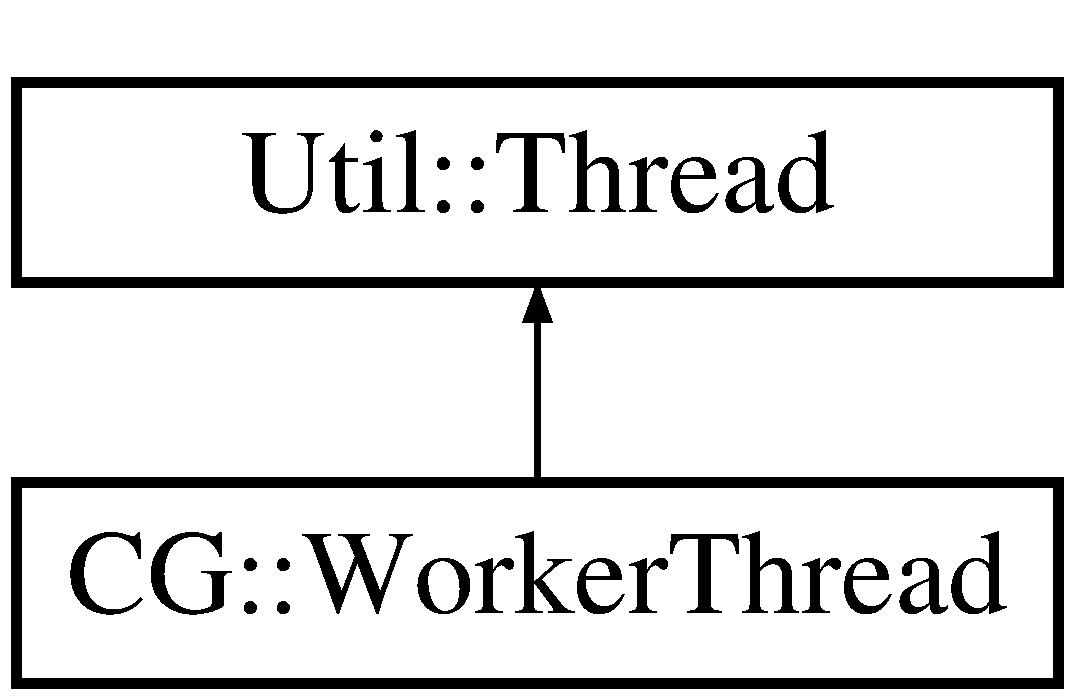
\includegraphics[height=2.000000cm]{class_c_g_1_1_worker_thread}
\end{center}
\end{figure}
\subsection*{Public Member Functions}
\begin{DoxyCompactItemize}
\item 
\mbox{\Hypertarget{class_c_g_1_1_worker_thread_a879675e8ca067dd8f4c86cd11323ec44}\label{class_c_g_1_1_worker_thread_a879675e8ca067dd8f4c86cd11323ec44}} 
{\bfseries Worker\+Thread} (bool is\+Multi\+Thread)
\item 
\mbox{\Hypertarget{class_c_g_1_1_worker_thread_a1af8c7be338769312b8ea32a7426dca2}\label{class_c_g_1_1_worker_thread_a1af8c7be338769312b8ea32a7426dca2}} 
bool {\bfseries initialize} ()
\item 
\mbox{\Hypertarget{class_c_g_1_1_worker_thread_a86a02f86edb87d8816ecf06560e0ecf0}\label{class_c_g_1_1_worker_thread_a86a02f86edb87d8816ecf06560e0ecf0}} 
void {\bfseries run} ()
\item 
\mbox{\Hypertarget{class_c_g_1_1_worker_thread_a82afd48da88b66a6d2a3082654302c9d}\label{class_c_g_1_1_worker_thread_a82afd48da88b66a6d2a3082654302c9d}} 
void {\bfseries push\+Data\+Packet} (\mbox{\hyperlink{class_c_g_1_1_data_packet}{Data\+Packet}} $\ast$data\+Packet)
\item 
\mbox{\Hypertarget{class_c_g_1_1_worker_thread_aae6cf77cf618a4513fea85a043fa381f}\label{class_c_g_1_1_worker_thread_aae6cf77cf618a4513fea85a043fa381f}} 
int {\bfseries get\+Data\+Packet\+Count} ()
\end{DoxyCompactItemize}
\subsection*{Public Attributes}
\begin{DoxyCompactItemize}
\item 
\mbox{\Hypertarget{class_c_g_1_1_worker_thread_a8e0c8febb197e68709d1c64e378159b1}\label{class_c_g_1_1_worker_thread_a8e0c8febb197e68709d1c64e378159b1}} 
\mbox{\hyperlink{class_util_1_1_queue}{Util\+::\+Queue}}$<$ \mbox{\hyperlink{class_c_g_1_1_data_packet}{Data\+Packet}} $\ast$ $>$ $\ast$ {\bfseries data\+Packet\+Queue}
\item 
\mbox{\Hypertarget{class_c_g_1_1_worker_thread_ae4b3ca99dc32ffe3670eace662ed8539}\label{class_c_g_1_1_worker_thread_ae4b3ca99dc32ffe3670eace662ed8539}} 
\mbox{\hyperlink{class_util_1_1_object_pool}{Util\+::\+Object\+Pool}}$<$ \mbox{\hyperlink{class_c_g_1_1_data_packet}{Data\+Packet}} $>$ $\ast$ {\bfseries data\+Packet\+Pool}
\item 
\mbox{\Hypertarget{class_c_g_1_1_worker_thread_a5634d8d0c007b15965b953034a9c015d}\label{class_c_g_1_1_worker_thread_a5634d8d0c007b15965b953034a9c015d}} 
\mbox{\hyperlink{class_util_1_1_object_pool}{Util\+::\+Object\+Pool}}$<$ \mbox{\hyperlink{class_c_g_1_1_buffer}{Buffer}} $>$ $\ast$ {\bfseries buffer\+Pool}
\item 
\mbox{\Hypertarget{class_c_g_1_1_worker_thread_abb23e83f2bd73c067cd5e4c6b25a910c}\label{class_c_g_1_1_worker_thread_abb23e83f2bd73c067cd5e4c6b25a910c}} 
std\+::list$<$ \mbox{\hyperlink{class_c_g_1_1_buffer}{Buffer}} $\ast$ $>$\+::iterator {\bfseries itr}
\end{DoxyCompactItemize}
\subsection*{Additional Inherited Members}


The documentation for this class was generated from the following files\+:\begin{DoxyCompactItemize}
\item 
network/core/Worker\+Thread.\+h\item 
network/core/Worker\+Thread.\+cpp\end{DoxyCompactItemize}

%--- End generated contents ---

% Index
\backmatter
\newpage
\phantomsection
\clearemptydoublepage
\addcontentsline{toc}{chapter}{Index}
\printindex

\end{document}
